% ******************************* PhD Thesis Template **************************
% Please have a look at the README.md file for info on how to use the template

\documentclass[a4paper,12pt,authoryear,print,index,custommargin,openany,oneside]{PhDThesisPSnPDF}

% ******************************************************************************
% ******************************* Class Options ********************************
% *********************** See README for more details **************************
% ******************************************************************************

% `a4paper'(The University of Cambridge PhD thesis guidelines recommends a page
% size a4 - default option) or `a5paper': A5 Paper size is also allowed as per
% the Cambridge University Engineering Deparment guidelines for PhD thesis
%
% `11pt' or `12pt'(default): Font Size 10pt is NOT recommended by the University
% guidelines
%
% `oneside' or `twoside'(default): Printing double side (twoside) or single
% side.
%
% `print': Use `print' for print version with appropriate margins and page
% layout. Leaving the options field blank will activate Online version.
%
% `index': For index at the end of the thesis
%
% `draftclassic': For draft mode without loading any images (same as draft in book)
%
% `draft': Special draft mode with line numbers, images, and water mark with
% timestamp and custom text. Position of the text can also be modified.
%
% `abstract': To generate only the title page and abstract page with
% dissertation title and name, to submit to the Student Registry
%
% `chapter`: This option enables only the specified chapter and it's references
%  Useful for review and corrections.
%
% ************************* Custom Page Margins ********************************
%
% `custommargin`: Use `custommargin' in options to activate custom page margins,
% which can be defined in the preamble.tex. Custom margin will override
% print/online margin setup.
%
% *********************** Choosing the Fonts in Class Options ******************
%
% `times' : Times font with math support. (The Cambridge University guidelines
% recommend using times)
%
% `fourier': Utopia Font with Fourier Math font (Font has to be installed)
%            It's a free font.
%
% `customfont': Use `customfont' option in the document class and load the
% package in the preamble.tex
%
% default or leave empty: `Latin Modern' font will be loaded.
%
% ********************** Choosing the Bibliography style ***********************
%
% `authoryear': For author-year citation eg., Krishna (2013)
%
% `numbered': (Default Option) For numbered and sorted citation e.g., [1,5,2]
%
% `custombib': Define your own bibliography style in the `preamble.tex' file.
%              `\RequirePackage[square, sort, numbers, authoryear]{natbib}'.
%              This can be also used to load biblatex instead of natbib
%              (See Preamble)
%
% **************************** Choosing the Page Style *************************
%
% `default (leave empty)': For Page Numbers in Header (Left Even, Right Odd) and
% Chapter Name in Header (Right Even) and Section Name (Left Odd). Blank Footer.
%
% `PageStyleI': Chapter Name next & Page Number on Even Side (Left Even).
% Section Name & Page Number in Header on Odd Side (Right Odd). Footer is empty.
%
% `PageStyleII': Chapter Name on Even Side (Left Even) in Header. Section Number
% and Section Name in Header on Odd Side (Right Odd). Page numbering in footer

% Uncomment to change page style
%\pagestyle{PageStyleII}

% ********************************** Preamble **********************************
% Preamble: Contains packages and user-defined commands and settings
\usepackage[pdftex,dvipsnames]{xcolor}
\hypersetup{colorlinks = true,
linkcolor = black,
urlcolor  = blue,
citecolor = black,
anchorcolor = black}
\urlstyle{sf}


% ******************************************************************************
% ****************************** Custom Margin *********************************

% Add `custommargin' in the document class options to use this section
% Set {innerside margin / outerside margin / topmargin / bottom margin}  and
% other page dimensions
\ifsetCustomMargin
  \RequirePackage[left=25mm,right=25mm,top=25mm,bottom=25mm]{geometry}
  \setFancyHdr % To apply fancy header after geometry package is loaded
\fi

% Add spaces between paragraphs
%\setlength{\parskip}{0.5em}
% Ragged bottom avoids extra whitespaces between paragraphs
\raggedbottom
% To remove the excess top spacing for enumeration, list and description
%\usepackage{enumitem}
%\setlist[enumerate,itemize,description]{topsep=0em}

% *****************************************************************************
% ******************* Fonts (like different typewriter fonts etc.)*************

% Add `customfont' in the document class option to use this section

\ifsetCustomFont
  % Set your custom font here and use `customfont' in options. Leave empty to
  % load computer modern font (default LaTeX font).
  %\RequirePackage{helvet}

  % For use with XeLaTeX
  %  \setmainfont[
  %    Path              = ./libertine/opentype/,
  %    Extension         = .otf,
  %    UprightFont = LinLibertine_R,
  %    BoldFont = LinLibertine_RZ, % Linux Libertine O Regular Semibold
  %    ItalicFont = LinLibertine_RI,
  %    BoldItalicFont = LinLibertine_RZI, % Linux Libertine O Regular Semibold Italic
  %  ]
  %  {libertine}
  %  % load font from system font
  %  \newfontfamily\libertinesystemfont{Linux Libertine O}
\fi

% *****************************************************************************
% **************************** Custom Packages ********************************

% ************************* Algorithms and Pseudocode **************************

%\usepackage{algpseudocode}


% ********************Captions and Hyperreferencing / URL **********************

% Captions: This makes captions of figures use a boldfaced small font.
%\RequirePackage[small,bf]{caption}

\RequirePackage[labelsep=space,tableposition=top]{caption}
\renewcommand{\figurename}{Fig.} %to support older versions of captions.sty


% *************************** Graphics and figures *****************************

%\usepackage{rotating}
%\usepackage{wrapfig}

% Uncomment the following two lines to force Latex to place the figure.
% Use [H] when including graphics. Note 'H' instead of 'h'
%\usepackage{float}
%\restylefloat{figure}

% Subcaption package is also available in the sty folder you can use that by
% uncommenting the following line
% This is for people stuck with older versions of texlive
%\usepackage{sty/caption/subcaption}
\usepackage{subcaption}

% ********************************** Tables ************************************
\usepackage{booktabs} % For professional looking tables
\usepackage{multirow}

%\usepackage{multicol}
%\usepackage{longtable}
%\usepackage{tabularx}


% *********************************** SI Units *********************************
\usepackage{siunitx} % use this package module for SI units


% ******************************* Line Spacing *********************************

% Choose linespacing as appropriate. Default is one-half line spacing as per the
% University guidelines

% \doublespacing
% \onehalfspacing
% \singlespacing


% ************************ Formatting / Footnote *******************************

% Don't break enumeration (etc.) across pages in an ugly manner (default 10000)
%\clubpenalty=500
%\widowpenalty=500

%\usepackage[perpage]{footmisc} %Range of footnote options


% *****************************************************************************
% *************************** Bibliography  and References ********************

%\usepackage{cleveref} %Referencing without need to explicitly state fig /table

% Add `custombib' in the document class option to use this section

%\usepackage{natbib}
%\setcitestyle{authoryear,open={(},close={)}}
%
%\ifuseCustomBib
%   %\RequirePackage[round, sort, numbers, authoryear]{natbib} % CustomBib
%   \usepackage{natbib}
%   \setcitestyle{authoryear,open={(},close={)}}
   

% If you would like to use biblatex for your reference management, as opposed to the default `natbibpackage` pass the option `custombib` in the document class. Comment out the previous line to make sure you don't load the natbib package. Uncomment the following lines and specify the location of references.bib file

%\RequirePackage[backend=biber, style=numeric-comp, citestyle=numeric, sorting=nty, natbib=true]{biblatex}
%\addbibresource{References/references} %Location of references.bib only for biblatex, Do not omit the .bib extension from the filename.
%
%\fi

% changes the default name `Bibliography` -> `References'
\renewcommand{\bibname}{References}


% ******************************************************************************
% ************************* User Defined Commands ******************************
% ******************************************************************************

% *********** To change the name of Table of Contents / LOF and LOT ************

%\renewcommand{\contentsname}{My Table of Contents}
%\renewcommand{\listfigurename}{My List of Figures}
%\renewcommand{\listtablename}{My List of Tables}


% ********************** TOC depth and numbering depth *************************

\setcounter{secnumdepth}{2}
\setcounter{tocdepth}{2}


% ******************************* Nomenclature *********************************

% To change the name of the Nomenclature section, uncomment the following line

%\renewcommand{\nomname}{Symbols}


% ********************************* Appendix ***********************************

% The default value of both \appendixtocname and \appendixpagename is `Appendices'. These names can all be changed via:

%\renewcommand{\appendixtocname}{List of appendices}
%\renewcommand{\appendixname}{Appndx}

% *********************** Configure Draft Mode **********************************

% Uncomment to disable figures in `draft'
%\setkeys{Gin}{draft=true}  % set draft to false to enable figures in `draft'

% These options are active only during the draft mode
% Default text is "Draft"
%\SetDraftText{DRAFT}

% Default Watermark location is top. Location (top/bottom)
%\SetDraftWMPosition{bottom}

% Draft Version - default is v1.0
\SetDraftVersion{v3.0}

% Draft Text grayscale value (should be between 0-black and 1-white)
% Default value is 0.75
%\SetDraftGrayScale{0.8}


% ******************************** Todo Notes **********************************
%% Uncomment the following lines to have todonotes.


\usepackage{xargs}

\usepackage[colorinlistoftodos,prependcaption,textsize=tiny]{todonotes}

\ifsetDraft
	%\usepackage[pdftex,dvipsnames]{xcolor}
	\newcommandx{\unsure}[2][1=]{\todo[linecolor=red,backgroundcolor=red!25,bordercolor=red,#1,inline]{#2}}
	\newcommandx{\change}[2][1=]{\todo[linecolor=blue,backgroundcolor=blue!25,bordercolor=blue,#1,inline]{#2}}
	\newcommandx{\info}[2][1=]{\todo[linecolor=OliveGreen,backgroundcolor=OliveGreen!25,bordercolor=OliveGreen,#1,inline]{#2}}
	\newcommandx{\improvement}[2][1=]{\todo[linecolor=Plum,backgroundcolor=Plum!25,bordercolor=Plum,#1,inline]{#2}}
	\newcommandx{\thiswillnotshow}[2][1=]{\todo[disable,#1,inline]{#2}}
	\newcommand{\mynote}[1]{\todo[inline]{#1}}
\else
	\newcommand{\mynote}[1]{}
	\newcommandx{\unsure}[2][1=]{}
	\newcommandx{\change}[2][1=]{}
	\newcommandx{\info}[2][1=]{}
	\newcommandx{\improvement}[2][1=]{}
	\newcommandx{\thiswillnotshow}[2][1=]{}
	%\newcommand{\listoftodos}{}
\fi

% Example todo: \mynote{Hey! I have a note}

% *****************************************************************************
% ******************* Better enumeration my MB*************
\usepackage{enumitem}

% My stuff added
\usepackage{parskip}
\setlength{\parindent}{1em}
\usepackage{amssymb}
\usepackage{lipsum}
\usepackage{layouts}
\usepackage{placeins}
\usepackage{pdflscape}
\usepackage{multirow}
\usepackage[ruled,vlined,linesnumbered]{algorithm2e}
\usepackage{array,ragged2e}
\usepackage{tikz}
\usepackage{afterpage}


%\usepackage[bitstream-charter]{mathdesign}
%\usepackage{charter} 

%\setlength{\parskip}{0em}

\usepackage{titlesec}
\titleformat{\chapter}[display]   
{\normalfont\huge\bfseries}{\chaptertitlename\ \thechapter}{20pt}{\Huge}   
\titlespacing*{\chapter}{0pt}{0pt}{40pt}

%*********** Table definitions ***********

\newcolumntype{L}[1]{>{\raggedright\let\newline\\\arraybackslash\hspace{0pt}}m{#1}}
\newcolumntype{C}[1]{>{\centering\let\newline\\\arraybackslash\hspace{0pt}}m{#1}}
\newcolumntype{R}[1]{>{\raggedleft\let\newline\\\arraybackslash\hspace{0pt}}m{#1}}

%*********** Math definitions ***********

\DeclareMathOperator{\p}{p}
\DeclareMathOperator{\Tr}{Tr}
\DeclareMathOperator{\InvGamma}{Inv-Gamma}
\DeclareMathOperator{\ELBO}{ELBO}
\DeclareMathOperator{\GP}{\mathcal{GP}}
\DeclareMathOperator{\PI}{PI}
\DeclareMathOperator{\EI}{EI}
\DeclareMathOperator{\UCB}{UCB}
\DeclareMathOperator{\BNN}{BNN}

\newcommand{\D}{\mathcal{D}}
\newcommand{\E}{\mathbb{E}}
\newcommand{\R}{\mathbb{R}}
\newcommand{\DKL}[2]{\mathcal{D}_{KL} \left( #1 \| #2 \right) }

% define datasets
\def\bostonvar{bostonHousing}
\def\bostonname{Boston Housing}

\def\concretevar{concrete}
\def\concretename{Concrete}

\def\energyvar{energy}
\def\energyname{Energy}

\def\kinvar{kin8nm}
\def\kinname{Kinematics 8nm}

\def\mnistvar{mnist}
\def\mnistname{MINST }

\def\navalnvar{naval-propulsion-plant}
\def\navalnname{Naval Propulsion Plant}

\def\powervar{power-plant}
\def\powername{Power Plant}

\def\proteinvar{protein-tertiary-structure}
\def\proteinname{Protein Tertiary Structure}

\def\winevar{wine-quality-red}
\def\winename{Wine Quality}

\def\yachtnvar{yacht}
\def\yachtname{Yacht}




% ************************ Thesis Information & Meta-data **********************
% Thesis title and author information, refernce file for biblatex
% ************************ Thesis Information & Meta-data **********************
%% The title of the thesis
\title{Architecture Search for Bayesian Neural Networks}
%\texorpdfstring is used for PDF metadata. Usage:
%\texorpdfstring{LaTeX_Version}{PDF Version (non-latex)} eg.,
%\texorpdfstring{$sigma$}{sigma}

%% Subtitle (Optional)
%\subtitle{Using the CUED template}

%% The full name of the author
\author{Michael Hutchinson}

%% Department (eg. Department of Engineering, Maths, Physics)
\dept{Department of Engineering}

%% University and Crest
\university{University of Cambridge}
% Crest minimum should be 30mm.
\crest{
\includegraphics[width=0.2\textwidth]{University_Crest}}
%% Use this crest, if you are using the college crest
%% Crest long miminum should be 65mm
\crest{
\includegraphics[width=0.45\textwidth]{University_Crest_Long}}

%% College shield [optional] 
% Crest minimum should be 30mm.
\collegeshield{
\includegraphics[width=0.2\textwidth]{CollegeShields/StJohns}}


%% Supervisor (optional)
%% for multiple supervisors, append each supervisor with the \newline command
\supervisor{Dr. Richard E. Turner}

%% Supervisor Role (optional) - Supervisor (default) or advisor
% \supervisorrole{\textbf{Supervisors: }}
%% if no title is desired:
% \supervisorrole{}

%% Supervisor line width: required to align supervisors
\supervisorlinewidth{0.35\textwidth}

%% Advisor (optional)
%% for multiple advisors, append each advisor with the \newline command
%\advisor{Dr. A. Advisor\newline
%Dr. B. Advisor}
     
%% Advisor Role (optional) - Advisor (default) or leave empty
% \advisorrole{Advisors: }
%% if no title is required
% \advisorrole{}

%% Advisor line width: required to align supervisors
%\advisorlinewidth{0.25\textwidth}


%% You can redefine the submission text:
% Default as per the University guidelines:
% ``This dissertation is submitted for the degree of''
\renewcommand{\submissiontext}{This report is submitted for the degree of}

%% Full title of the Degree
\degreetitle{Master of Engineering}

%% College affiliation (optional)
\college{Christ's College}

%% Submission date
% Default is set as {\monthname[\the\month]\space\the\year}
%\degreedate{September 2014} 

%% Meta information
\subject{LaTeX} \keywords{{LaTeX} {PhD Thesis} {Engineering} {University of
Cambridge}}


% ***************************** Abstract Separate ******************************
% To printout only the titlepage and the abstract with the PhD title and the
% author name for submission to the Student Registry, use the `abstract' option in
% the document class.

\ifdefineAbstract
 \pagestyle{empty}
 \includeonly{Declaration/declaration, Abstract/abstract}
\fi

% ***************************** Chapter Mode ***********************************
% The chapter mode allows user to only print particular chapters with references
% Title, Contents, Frontmatter are disabled by default
% Useful option to review a particular chapter or to send it to supervisior.
% To use choose `chapter' option in the document class

\ifdefineChapter
 \includeonly{Chapter3/chapter3}
\fi

% ******************************** Front Matter ********************************
\begin{document}

\frontmatter

\maketitle

%% ******************************* Thesis Dedidcation ********************************

\begin{dedication} 

I would like to dedicate this thesis to my loving parents \dots

\end{dedication}


%% ******************************* Thesis Declaration ***************************

\begin{declaration}

I hereby declare that except where specific reference is made to the work of 
others, the contents of this dissertation are original and have not been 
submitted in whole or in part for consideration for any other degree or 
qualification in this, or any other university. This dissertation is my own 
work and contains nothing which is the outcome of work done in collaboration 
with others, except as specified in the text and Acknowledgements. This 
dissertation contains fewer than 12,000 words including appendices, footnotes, tables and equations and has fewer than 50 pages.

% Author and date will be inserted automatically from thesis.tex \author \degreedate

\end{declaration}


% ************************** Thesis Acknowledgements **************************

\begin{acknowledgements}      


Not sure if I need to put stuff in here - whether this is a technical matter or not.

People I might mention:
\begin{itemize}
	\item Siddharth
	\item Marcin
	\item Thang
\end{itemize}


\end{acknowledgements}

% ************************** Thesis Abstract *****************************
% Use `abstract' as an option in the document class to print only the titlepage and the abstract.
\begin{abstract}
	\normalsize
	Standard neural networks have revolutionised the machine learning field, improving performance by orders of magnitude over previous methods in a wide variety of applications, particularly in tasks with significant quantities of data. A key part of the success of these methods has come from designing bespoke architectures, which also work well with deep learning optimisation methods. As the size of neural networks has increased significantly, the task of designing these networks by hand has become increasingly more difficult and time consuming. 
	
	Automated methods of performing architecture search have therefore been developed, and this topic has seen a significant body of work in the last 3 years. None of this work however has been to be applied to Bayesian Neural Networks. These probabilistic counterparts hold several key advantages over regular neural networks. They provide well calibrated uncertainty estimates in their predictions, they are significantly more robust to tampering via adversarial samples, and a range of useful additions, such as continual learning, distributed learning and active learning can be applied readily without any modification. Additionally, there has been little systematic study into how the various hyper-parameters associated with Bayesian Neural Networks affect model performance. 
	
	This report has two main groups of contributions.
	
	First, a detailed study of the effects of various hyper-parameters on the performance of MLP structure BNNs, and identification of systematic trends. We find that layer width and depth are both important factors. Networks that are too large can be detrimental to performance. The effect of the amount of data in the training set has on model optimisation is also investigated. It is shown that the balance between model size and data size is important in controlling the under-fitting or over-fitting of models. Finally the effects of pruning in VI BNNs investigated, and the manner in which the optimiser makes the trade off between reconstruction loss and prior fit terms. We find that in larger networks, many of the weights are pruned completely out the model, reducing the model to a minimum descriptive length, or in some cases further.
	
	Second, is a new method for searching for optimal MLP structure networks in Bayesian Neural Networks, a task currently untackled. This method robustly outperforms the random search on the majority of tasks, excepting cases where the noise from randomness in training BNNs is too great. In most tasks it is as good as, or marginally better than simply performing Bayesian optimisation over the final performance of the BNNs. 
\end{abstract}


% *********************** Adding TOC and List of Figures ***********************

\tableofcontents

A pdf version of this report can be found at 

%\listoffigures

%\listoftables

% \printnomenclature[space] space can be set as 2em between symbol and description
%\printnomenclature[3em]

%\printnomenclature
%\improvement{Should I fill out this nomenclature section?}

%\listoftodos[Notes]

% ******************************** Main Matter *********************************
\mainmatter

%!TEX root = ../thesis.tex
%*******************************************************************************
%*********************************** First Chapter *****************************
%*******************************************************************************

\chapter{Introduction}  %Title of the First Chapter

\ifpdf
    \graphicspath{{Chapter1/Figs/Raster/}{Chapter1/Figs/PDF/}{Chapter1/Figs/}}
\else
    \graphicspath{{Chapter1/Figs/Vector/}{Chapter1/Figs/}}
\fi

Standard neural networks have revolutionised the machine learning field, improving performance by orders of magnitude over previous methods in a wide variety of applications, particularly in tasks with significant quantities of data. A key part of the success of these methods has come from designing bespoke architectures, which also work well with deep learning optimisation methods. The design of these networks has two distinct parts: the choice of building blocks for the networks, and the structure in which these blocks are connected together.

The design of new building blocks has been the main driver in performance of these networks. Generally these have increased performance in one of two ways. 

Firstly, by providing a significant reduction in the number of parameters of the network while maintaining the networks level of expressibility on a given task. Since these layers are usually a constrained form of a fully connected layer, this could also be viewed as providing a form of "hard regularisation" in the network by building in invariance in sensible ways. Examples of this include conventional layers, building in local connectivity and translation invariance or recurrent networks, building in time invariance. Designing these new layers has yet to be automated, and given the ingenuity involved in doing so, it is unlikely this will happen in the near future. 

Secondly, by improving the optimisation of neural networks with gradient based methods. Examples of this include the use of the RELU unit, residual layers, skip connections and highway connections.

The configuration in which these building blocks are connected together, and the various hyper-parameters associated with them, are also important. The configuration of these blocks defines the "predictive power" of the network, and encodes a prior belief about how the outputs should be predicted from the inputs. This configuration can play a significant role in the performance of neural networks; for example the progression from LeNet \citep{LeCun1989} to AlexNet \citep{NIPS2012_4824} to the Inception line of architectures \citep{DBLP:journals/corr/SzegedyLJSRAEVR14,DBLP:journals/corr/SzegedyVISW15,DBLP:journals/corr/SzegedyIV16} is largely a result of connecting convolution filters, pooling and fully connected layers in different configurations, showing that this is a significant factor. 

The purpose of architecture search therefore is to explore some defined space of possible architectures and find architectures that perform best. This is a non-trivial process. Usually the search space is extremely large, and individual architectures expensive to evaluate. Traditionally this search has been done by hand, utilising human intuition. This has therefore led to a situation where significant amounts of research time are  spent testing different configurations of neural networks, looking for minor improvements. Benefits of an automated approach to architecture search are
\begin{itemize}
	\item[\( \diamond \)] A reduction in research time spent directly on searching for incrementally better architectures. An automated procedure could take over the larger part of the menial work on this task, freeing research time for alternative pursuits.
	\item[\( \diamond \)] A reduction in the influence of human bias on the search procedure. Human designers of networks have a preference for regular and seemingly ordered structures for neural networks. As can be observed in many architecture search papers \cite{Baker2016,Brock2017,zoph2016neural,zoph2018learning}, these are often not optimal architectures. Automated methods would explore the space of architectures without this particular bias.
	\item[\( \diamond \)] An ability to tailor models to specific problems. Much of the work carried out discovering new architectures consists of looking at performance on a single dataset and transferring the architectures discovered on these datasets to other problems. This can introduce data specific bias into the architectures used. An automated method with little human interaction required could be used to tailor networks to specific problems for better performance. 
\end{itemize}

The case for automated architecture search is clear, and there has been substantial work in this area, which will be discussed later. However, none of this work has looked at architecture search for designing Bayesian Neural Networks (BNNs). This Bayesian interpretation of neural networks has several attractive properties in contrast to regular neural networks. To name a few:
\begin{itemize}
	\item[\( \diamond \)] BNNs provide uncertainty estimates in their predictions. In comparison to standard neural networks which produce point estimates, or can be confidently wrong when using softmax layers in classification, BNNs provide well-calibrated uncertainty in their predictions as a result of their probabilistic formulation. These uncertainty estimates provide advantages in making decisions in situations where there is significant risk in making incorrect prediction, such as medicine or finance, or in exploration-based tasks such as reinforcement learning. 
	\item[\( \diamond \)] BNNS are more robust to a series of effects that exploit the highly specific configuration of weights in a neural network, such as adversarial attacks  \citep{Liu2018}. This robustness comes from integrating or sampling across the posterior parameter space.
	\item[\( \diamond \)] Due to the probabilistic nature of the weights, several techniques have been developed for probabilistic models that cannot be applied to regular neural networks without some modification, such as continual learning \citep{Swaroop2019}, distributed learning \citep{Bui} or active learning, which can be applied to BNNs readily.
\end{itemize}

BNNs do have some downsides. They are usually significantly more expensive to train than regular neural networks. Due to the probabilistic, but intractable, nature of the weights, many Monte Carlo samples are generally required to produce good gradient and prediction estimates. This additional cost at present has prevented these methods from being scaled up to typical deep neural network sizes. The training of BNNs can also be tricky to get right, particularly in finding good hyper-parameter settings and architecture sizes which do not lead to over-fitting or under-fitting. As a result of these reasons, BNNs are yet to see wide spread adoption. 

The advantages of BNNs and the lack of work on architecture search on them naturally leads to the topic of this project. The first aim is to provide a characterisation of the performance of fully connected networks, trained under a Variational Inference framework (VI) \nomenclature[z-VI]{VI}{Variational Inference} The objective of this is to provide a preliminary investigation into how the various hyper-parameters of this particular space affect network performance. Given the very large search space and the inefficiency in exploring this manually, the second aim is to investigate automatic methods of exploring the search space.
%!TEX root = ../thesis.tex
%*******************************************************************************
%****************************** Second Chapter *********************************
%*******************************************************************************

\chapter{Introductory Material}

\ifpdf
    \graphicspath{{Chapter2/Figs/Raster/}{Chapter2/Figs/PDF/}{Chapter2/Figs/}}
\else
    \graphicspath{{Chapter2/Figs/Vector/}{Chapter2/Figs/}}
\fi

\section{Variational Inference for BNNs}

The objective of this project its to provide a form for searching for optimal architectures of Bayesian Neural Networks. The methodology of training these is diverse and can lead to significant differences in performance. Variational Inference was selected as the methodology for training for two reasons: it produces state of the art results on many problems \citep{bui2016deep}; and it is the most scalable method for BNNs at present, able to scale up to at least the size of medium-sized convolutions networks \citep{Shridhar2018}.

Unlike the training of standard neural networks, the training of Bayesian Neural Networks (BNNs) is not a straightforward task. In standard neural networks we have a series of point weights \( \mathbf{w} \) for which we optimise the predictions of some output \( \mathbf{y}_i \) for some input data \( \mathbf{x}_i \), drawn from a dataset \( \D = \{\mathbf{x}_i, \mathbf{y}_i\}_{i=1}^N \). In the Bayesian interpretation, we place distributions over the weights of the parameters in the network, and attempt to maximise the likelihood of the data observed. This likelihood can be found by taking the expectation with respect to the weights of the joint likelihood
\begin{align}
	P(\mathbf{y} | \mathbf{x}) = \E_{P(\mathbf{w} | \mathbf{y}, \mathbf{x})} \left[ P(\mathbf{y}, \mathbf{w} |  \mathbf{x}) \right]
\end{align} 
This calculation is, with the exception of very simple cases, highly intractable when our prediction for \( \mathbf{y} \) comes from a neural network. As such, it is necessary to use approximations to be able to compute this likelihood, and to be able to maximise it with respect to the weight distributions.

The form utilised in this project is a variational approximation. This simplifies the above expression by introducing a variational distribution, \( q_\phi(\mathbf{w}) \), over the weights of a form that is more simple to work with. This is developed by \citet{Hinton1993, graves2011practical}. Here the log likelihood is maximised, as it is easier.
\begin{align}
	\log P(\mathbf{y} | \mathbf{x}) &= 
	\int \log  \left[P(\mathbf{y}, \mathbf{w} | \mathbf{x}) \right] d \mathbf{w}\\
	&= \int \log \left[P(\mathbf{y} |  \mathbf{w}, \mathbf{x})P(\mathbf{w}) \frac{q_\phi(\mathbf{w})}{q_\phi(\mathbf{w})}\right] d \mathbf{w}\\
	&\geq \int q_\phi(\mathbf{w}) \log \left[ \frac{P(\mathbf{y} |  \mathbf{w}, \mathbf{x})P(\mathbf{w})}{q_\phi(\mathbf{w})}\right] d \mathbf{w} \label{eq:jensens1}\\
	&= \int q_\phi(\mathbf{w}) \log \left[ P(\mathbf{y} |  \mathbf{w}, \mathbf{x})\right] d \mathbf{w} - \int q_\phi(\mathbf{w}) \log \left[ \frac{q_\phi(\mathbf{w})}{P(\mathbf{w})}\right] d \mathbf{w}\\
	&= \E_{q_\phi(\mathbf{w})}\left[ \log P(\mathbf{y} |  \mathbf{w}, \mathbf{x}) \right] - \DKL{q_\phi(\mathbf{w})}{P(\mathbf{w})}
\end{align}
Equation \ref{eq:jensens1} uses Jensen's inequality and \( \DKL{\cdot}{\cdot} \) is the KL-divergence. These terms are commonly called the reconstruction loss and the prior fit terms. This bound is known as the \textit{Variational Free Energy} or the \textit{Expected Lower Bound (ELBO)}. Two alternative interpretations of this exist. First, as a \textit{minimum descriptive length} \citep{Hinton1993} method for training neural networks, by minimising the amount of information encoded in the weights. Second, it can be shown that minimising this lower bound on the log likelihood is equivalent to minimising the KL divergence \( \DKL{q_\phi(\mathbf{w})}{P(\textbf{w}| \mathbf{x}, \mathbf{y})} \), i.e. the distance between the posterior weight distribution and the variational distribution, indicating this is a sensible lower bound.

These terms however are not always tractable. Using \citet{Blundell2015} we approximate the terms with a Monte Carlo estimate, drawing samples from \( q_\phi(\mathbf{w}) \).
\begin{align}
\E_{q_\phi(\mathbf{w})}&\left[ \log P(\mathbf{y} |  \mathbf{w}, \mathbf{x}) \right] - \DKL{q_\phi(\mathbf{w})}{P(\mathbf{w})} \nonumber \\
&\approx \frac{1}{N} \sum_{i=1}^{N} \log \left[ P(\mathbf{y} |  \mathbf{w}_i, \mathbf{x}) \right]  - \log \left[ \frac{q_\phi(\mathbf{w}_i)}{P(\mathbf{w})} \right], \; \mathbf{w}_i \sim q_\phi(\mathbf{w}_i)
\end{align}
In our experiments, 10 samples are used at train time and 100 at test time. Computing \( \log P(\mathbf{y} |  \mathbf{w}_i, \mathbf{x}) \) relies on deciding a form of this distribution. Here we model this homoskedastic noise, \(P(\mathbf{y} |  \mathbf{w}_i, \mathbf{x}) = \mathcal{N}(f_{\mathbf{w}_i}(\mathbf{x}), \sigma_y^2) \), with the parameter \( \sigma_y^2 \) joint optimised with the weights. An alternative option for this is using a second head to predict the variance as well. \citet{Blundell2015} shows then that standard back propagation techniques can be used to train the parameters \( \phi \) of the \( q_\phi(\mathbf{w}) \) distribution and \( \sigma_y^2 \).

Unfortunately this estimator has very high variance. Two things can be done to reduce this. First, by constraining our variational distribution \( q_\phi(\mathbf{w}) \) and prior \( P(\mathbf{w}) \) to be Gaussian distributions, there is a tractable form for the KL divergence between 2 instances. For a pair of \( d \)-dimensional Normal distributions

\begin{align}
	&\DKL{\mathcal{N}(\mathbf{\mu}_1, \mathbf{\Sigma}_1)}{\mathcal{N}(\mathbf{\mu}_2, \mathbf{\Sigma}_2)}) \nonumber \\
	&= \frac{1}{2} \left[\log \frac{|\mathbf{\Sigma}_2|}{|\mathbf{\Sigma}_1|} - d  + \Tr \left( \mathbf{\Sigma}_1^{-1} \mathbf{\Sigma}_2 \right) + (\mathbf{\mu}_1 - \mathbf{\mu}_2)^T \mathbf{\Sigma}_2^{-1} (\mathbf{\mu}_1 - \mathbf{\mu}_2) \right]
\end{align}
Second, by employing the reparametisation trick of \citet{Kingma2015}. Assuming our weights in a given layer are independently distributed, we write them as
\begin{align}
	w_{i,j} = \mu_{i,j} + \sigma_{i,j} \epsilon_{i,j}, \quad \epsilon_{i,j} \sim \mathcal{N}(0,1)
\end{align}
This changes the variance of the estimator from being independent of batch size, to being inversely proportional to the size of the batch. Together, these lead to significantly better empirical results.

Additionally, since the weights only affect the model prediction thought the activation of the neuron they connect to, we can write the output of that neuron as the sum of the weights times the input activations. For a layer with \( J \) inputs,
\begin{align}
	b_i = \sum_{j=1}^{J} w_{i,j} a_j
\end{align}
Since this is just the sum of scaled Gaussians, the result will also be a Gaussian.
\begin{align}
	b_i &\sim \mathcal{N}(\gamma_i, \delta_i)\\
	\gamma_i &= \sum_{j=1}^{J} a_j \mu_{i,j} \qquad \delta_i \sum_{j=1}^{J} = a_j^2 \sigma_{i,j}^2
\end{align}
Instead of sampling each weight and summing, we can therefore perform the two sums above and only sample the output distributions. Sampling the weights requires \( J^2 \) samples, whereas sampling the outputs only requires \( J \) samples, a significant reduction, especially in larger networks. This is the \textit{local} reparametisation trick.

The final improvement used in later experiments is the use of \textit{hyper-priors} on the width of the priors in the network. With Gaussian priors, the width of the prior can have a significant effect on the performance of the network, and adds an additional parameter to optimise over in the search space for architectures. There rigorous is no way to determine what the optimal width will be \textit{a priori}, beyond intuition. By introducing hyper-priors on the prior width we can optimise the prior width at train time and avoid having to add this parameter to the search space. We follow the method set out in \citet{wu2018fixing}. In this case the hierarchical prior takes the form 
\begin{align}
	\mathbf{s} \sim P(\mathbf{s}), \quad \mathbf{w} \sim P(\mathbf{w}| \mathbf{s})
\end{align}
Allowing too many degrees of freedom in the hyper-priors can be detrimental, so a single hyper-prior is introduced per layer, covering all the weights in that layer (labelled \( s_\lambda \) for the hyper-prior on layer \( \lambda \)). The hyper-priors are inverse-Gamma distributed to be conjugate priors to the independent Gaussian distributions of the weights.
\begin{align}
	s_\lambda \sim \InvGamma(\alpha, \beta), \quad \mathbf{w}_\lambda \sim \mathcal{N}(\mathbf{0}, s_\lambda\mathbf{I}) 
\end{align}
Our new ELBO is simply
\begin{align}
\E_{q_\phi(\mathbf{w})}\left[ \log P(\mathbf{y} |  \mathbf{w}, \mathbf{x}) \right] - \DKL{q_\phi(\mathbf{w})}{P(\mathbf{w}| \mathbf{s})P(\mathbf{s})}
\end{align}
As an approximation, at each update step Type-2 empirical Bayes is used to estimate the MAP solution for the prior width to provide the tightest ELBO.
\begin{align}
	s^*_\lambda = \arg\min_{\mathbf{s}_\lambda} \left[ \DKL{q_\phi(\mathbf{w}_\lambda)}{P(\mathbf{w}_\lambda| s_\lambda)} - \log s_\lambda  \right]
\end{align} 
There is a closed form solution to this optimisation
\begin{align}
	s^*_\lambda = \frac{\Tr \left[ \mathbf{\Sigma}^q_\lambda+ \mathbf{\mu}^q_\lambda (\mathbf{\mu}^q_\lambda)^T \right] + 2\beta}{N_\lambda + 2 \alpha + 2}
\end{align}
Where  \( N_\lambda \) is the number of weights under the prior \( s_\lambda \). \citep{wu2018fixing} shows that this method is almost as good as or better than manual tuning of the prior width for the standard UCI datasets.

One drawback of BNNs is their significant cost in training. Compare to regular neural networks they can take significantly more optimisation steps to converge. One of the main reasons for picking the variational form of BNNs with mean field weight is for the scalability in network size they present. Even these, however, are orders of magnitude slower than regular neural networks. Significant parts of these costs come from the sampling required during training, and the multiple evaluations of the network for each data-point required to produce good gradient estimates.

BNNs generally have large numbers of hyper-parameters associated with architecture and training. If we consider MLPs, we have to choose a number of layers, a width for each layer, the activation functions, and the form of prior and variational distribution. Some of these are constrained by methodology, but many are free to be chosen. If we also consider the optimisation, we generally must pick a learning rate and possibly other parameters as well. Even for these small scale architectures, it therefore makes sense to utilise some kind of automated search method.

\section{Bayesian Optimisation}
The body of scientific literature focused on the optimisation of some function \( f(\mathbf{x}) \) over some set of possibility \( \mathcal{A} \) is extensive. Simply
\begin{align}
	\max_{\mathbf{x \in \mathcal{A} \subset \R^n}} f(x)
\end{align}
The large part of this assumes that \( f(\mathbf{x}) \) contains some particular property in combination with the bounds of \( \mathcal{A} \), such as convexity, a known mathematical representation, or cheapness to evaluate. 

While some problems in machine learning have applications for these techniques, not all do. The assumptions of cheapness is used in the gradient-based update methods used for many algorithms, but due to the large number of iterations usually required to converge models, the overall training of machine learning models becomes incredibly expensive. This makes the results of trained algorithms comparatively expensive and usually an objective function that one might cast on the results of these, such as finding optimal hyper-parameter setting for an algorithm for accuracy, a non-convex function in its inputs. Most standard efficient optimisation methods are therefore inappropriate for performing meta-tasks on the hyper-parameters of machine learning algorithms.

Bayesian Optimisation is a powerful method for finding the maxima or minima of black box functions with expensive objectives with no special structure to the objective efficiently. It is also a gradient-free method, and so can handle situations where the gradients of the objective with respect to the parameters is intractable. Finally it is possible to handle, to a degree, noisy evaluations of the objective function with this method.

These properties have made Bayesian Optimisation a key method in applications such as clinical trials and finance, and also make them suitable to the architecture search problem.

Bayesian optimisation relies on the Bayesian inference of the most likely model (\( M \)) of the data, given the evidence seen (\( E \)). This can be done via Bayes rule
\begin{align}
	P(M|E) \propto P(E|M)P(M)
\end{align}
To do this we on placing a prior over the possible functions that could describe the data, \( P(M) \), and computing the likelihood of the evidence seen under these models, \( P(E|M) \). In terms of a function that might model the data, \( f \), and our observed data so far, \( \mathcal{D}_{1:t} = \{\mathbf{x}_i, \mathbf{y}_i\}_{i=1}^t \)
\begin{align}
	P(f|\mathcal{D}_{1:t}) \propto P(\mathcal{D}_{1:t} | f)P(f)
\end{align}
The Bayesian optimisation process is then an iterative one. Taking the distribution over functions, we maximise some objective function, usually called the \textit{acquisition function}, with respect to this distribution and sample the new point at the optima of the acquisition function. Algorithm \ref{alg:bo} set out the simple procedure for performing Bayesian optimisation.

\begin{algorithm}[t]
	\footnotesize
	\For{t=1,2, ...}{
		Compute the posterior likelihood \( P(f|\mathcal{D}_{1:t}) \)
		
		Find \( \mathbf{x}_t \) by optimising the aquisition function over the seen data, \begin{align}
			\mathbf{x}_t = \arg\min_{\mathbf{x}} u_{f(\mathbf{x}) \sim P(f|\mathcal{D}_{1:t})}(\mathbf{x}|\mathcal{D}_{1:t-1})
		\end{align}
		
		Sample the objective function \( y_t = f(\mathbf{x}_t) + \epsilon_t \)
		
		Update the dataset \( \mathcal{D}_{1:t}  = \{ \mathcal{D}_{1:t-1}, (\mathbf{x}_t, y_t)  \}\)
	}
		
	\caption{Bayesian Optimisation}
	\label{alg:bo}
\end{algorithm}

Two questions are raised by this: how to perform the inference of \( P(f|\mathcal{D}_{1:t}) \), and what form the acquisition function should take. A discussion of both questions follows.

\subsection{Gaussian Processes as function priors}
Gaussian Processes are an elegant way to deal with inferring a distribution over possible functions from some observations and a prior. The prior over the function is defined by some mean function on \( \mathbf{x} \), \( m(\cdot) \), and some covariance function between data-points, \( k(\cdot, \cdot) \)
\begin{align}
	f(\mathbf{x}) \sim \GP(m(\mathbf{x}), k(\mathbf{x}, \mathbf{x}'))
\end{align}

In essence this returns the mean and variance of a Normal distribution for a given point \( \mathbf{x} \). It is usual to set the mean function to zero, both for convenience and the fact that for data we know little about, this is likely the best assumption (in particular if we normalise observed data). This leaves us just with the choice of covariance function. 

In the predictive setting, we want to infer predictions about new data points from previously seen data. We know that all points on our function \( f \) are jointly Gaussian. If we have observed the points \( \mathbf{x}_{1:t}, \mathbf{f}_{1:t} \) and wish to make predictions about \( f_{t+1}(\mathbf{x}_{t+1}) \) then we can write
\begin{align}
	\begin{bmatrix}
		\mathbf{f}_{1:t} \\
		f_{t+1}
	\end{bmatrix}
	\sim 
	\mathcal{N} \left( \mathbf{0}, 
	\begin{bmatrix}
		\mathbf{K} & \mathbf{k}\\
		\mathbf{k}^T & k(\mathbf{x}_{t+1}, \mathbf{x}_{t+1})
	\end{bmatrix} \right)
\end{align}
where 
\begin{align}
	\mathbf{K} &= \begin{bmatrix}
		k(\mathbf{x}_1, \mathbf{x}_1) & k(\mathbf{x}_1, \mathbf{x}_2) & \cdots & k(\mathbf{x}_1, \mathbf{x}_t)\\
		k(\mathbf{x}_2, \mathbf{x}_1)& k(\mathbf{x}_2, \mathbf{x}_2) & \cdots & k(\mathbf{x}_2, \mathbf{x}_t)\\
		\vdots & \vdots & \ddots & \vdots\\
		k(\mathbf{x}_t, \mathbf{x}_1)& k(\mathbf{x}_t, \mathbf{x}_2) & \cdots & k(\mathbf{x}_t, \mathbf{x}_t)\\
	\end{bmatrix}
	\\
	\mathbf{k} &= \begin{bmatrix}
	k(\mathbf{x}_{t+1}, \mathbf{x}_1)& k(\mathbf{x}_{t+1}, \mathbf{x}_2) & \cdots & k(\mathbf{x}_{t+1}, \mathbf{x}_t)
	\end{bmatrix}
\end{align}
Using the  Sherman-Morrison-Woodbury formula we can compute the distribution of \( f_{t+1}(\mathbf{x}_{t+1}) \)
\begin{align}
	f_{t+1}(\mathbf{x}_{t+1}) \sim \mathcal{N}(\mu_t(\mathbf{x}_{t+1}), \sigma^2_t(\mathbf{x}_{t+1}))
\end{align}
where
\begin{align}
	\mu_t(\mathbf{x}_{t+1}) &= \mathbf{k}^T\mathbf{K}^{-1}\mathbf{f}_{1:t}\\
	\sigma_t^2(\mathbf{x}_{t+1}) &= k(\mathbf{x}_{t+1}, \mathbf{x}_{t+1}) - \mathbf{k}^T\mathbf{K}^{-1}\mathbf{k}
\end{align}
Note that once \( \mathbf{K}^{-1} \) has been computed, and this is an \( \mathcal{O}(n^3) \) operation, then computing \( \mu_t(\mathbf{x}_{t+1}) \) and \( \sigma_t^2(\mathbf{x}_{t+1}) \) is comparatively fast as it only involves computing kernels and linear matrix multiplications. This means predicting multiple points comes at little additional cost compared to a single point. If we wish to model some noise \( \sigma_y^2 \) on the function, then the equations become
\begin{align}
	\mu_t(\mathbf{x}_{t+1}) &= \mathbf{k}^T \left(\mathbf{K} + \sigma_y^2\mathbf{I} \right)^{-1} \mathbf{f}_{1:t}\\
	\sigma_t^2(\mathbf{x}_{t+1}) &= k(\mathbf{x}_{t+1}, \mathbf{x}_{t+1}) - \mathbf{k}^T\left(\mathbf{K} + \sigma_y^2\mathbf{I} \right)^{-1}\mathbf{k}
\end{align}
and this parameter \( \sigma_y^2 \) can be optimised like any other parameter.

A more in depth treatment of GPs can be found in \citet{williams2006gaussian}.

The choice of kernel then is the prior that we place on the function, and the conditioning on the data our computation of the likelihood of different models having observed some data. We can then observe the distribution of the posterior by sampling from it at points of interest, as described above.

The choice of kernel is an area with significant literature. In this project we use  Exponential Quadratic (EQ) kernels and Linear kernels. EQ kernels have become a default choice for GPs as they have several attractive properties: it is infinitely smooth in its derivatives, and it has only two hyper-parameters. It has the form
\begin{align}
	k_{SE}(x, x') = \sigma^2 \exp\left(-\frac{(x - x')^2}{l^2}\right)
\end{align} 
The two hyper-parameters are:
\begin{itemize}
	\item[\( l \)]  - The length scale controls the length scale of the function, how fast the function will change with respect to its inputs.
	\item[\( \sigma \)] - The output variance determines the average distance of the function from the mean.
\end{itemize}

The linear kernel has the form
\begin{align}
	k_{Lin}(x, x') = \sigma_b^2 + \sigma_v^2(x-c)(x'-c)
\end{align}
This has 3 hyper-parameters:
\begin{itemize}
	\item[\( \sigma_b^2 \)] - This places a prior on how far from 0 the hight of the function will be when \( x = c \) or \( x' = c \), akin to the intercept.
	\item[\( \sigma_v^2 \)] - This determines the functions average distance from the mean.
	\item[\( c \)] - This determines the x coordinate at which all posterior function lines will pass through. At this point the function will only have covariance from \( \sigma_b^2 \) and noise.
\end{itemize}

We use additive combinations of these kernels to produce more powerful function priors. 

The choice of hyper-parameters in the chosen kernel has a significant effect on the form of the posterior function. It is therefore common to iteratively optimise these hyper-parameters to optimise the train set log-likelihood.

More information on different kernels, and an excellent guide on kernel choice, see \citet{duvenaud2014automatic}. \citet{williams2006gaussian} also contains information on more complex kernels, combing kernels and advanced GP methods.

\subsection{Acquisition functions}

Three main acquisition functions are considered, and are the most commonly used in Bayesian Optimisation. These are the Expected Improvement (EI) function, the Probability of Improvement (PI) function and the Upper Confidence Bound function (UCB). 

\subsubsection{Probability of Improvement}

The most intuitive of these is the Probability of Improvement function \citep{kushner1964new}. This is simply the probability that a given point will be better than the current best point.
\begin{align}
	\PI(\mathbf{x}) = Pr(f(\mathbf{x}) \geq f(\mathbf{x}^+)
\end{align}
Where \( f(\mathbf{x}^+) \) is the value of the best point found so far. This is exactly
\begin{align}
	\PI(\mathbf{x}) = \Phi\left(\frac{\mu(\mathbf{x}) - f(\mathbf{x}^+)}{\sigma(\mathbf{x})}\right)
\end{align}
with \( \Phi(\cdot) \) as the Normal cumulative density function. This is an inherently highly exploitative function, and will always pick the most likely place to get a gain. Points with a small variance and slightly higher mean than the best point will be favoured over those with higher variance and mean, leading to strong exploration of local maxima and less likelihood of exploration far away from local maxima. This can present issues if a local maximum is not globally maximal. This is best seen by considering PI in another form. If we consider the reward for a given point as
\begin{align}
	R(\mathbf{x}) = \begin{cases}
	 1 & f(\mathbf{x}) > f(\mathbf{x}^+)\\
	 0 & f(\mathbf{x}) \leq f(\mathbf{x}^+)
	\end{cases}
\end{align}
Taking the expectation of this with respect to the current GP posterior at point \( \mathbf{x} \) gives us
\begin{align}
	\E_{f(\mathbf{x}) \sim \GP(\mu(\mathbf{x}), \sigma^2(\mathbf{x})| \mathcal{D})}\left[  R(\mathbf{x}) \right] = \Phi\left(\frac{\mu(\mathbf{x}) - f(\mathbf{x}^+)}{\sigma(\mathbf{x})}\right)
\end{align}

\subsubsection{Expectation of Improvement}
This leads to the form of the second acquisition function, Expected Improvement \citep{jones1998efficient, mockus1978toward}. Instead of defining the reward as rewarding any improvement, the reward is defined as the amount it will improve over the current best point
\begin{align}
	R(\mathbf{x}) = \max\left[0, f(\mathbf{x}) - f(\mathbf{x}^+)\right]
\end{align}
Taking the expectation of this over the distribution of \( f(\mathbf{x}) \)
\begin{align}
	\E&_{f(\mathbf{x}) \sim \GP(\mu(\mathbf{x}), \sigma^2(\mathbf{x})| \mathcal{D})}\left[  R(\mathbf{x}) \right] \\
	&= \int_{f(\mathbf{x}^+)}^{\infty} (f(\mathbf{x}) - f(\mathbf{x}^+)) \mathcal{N}(f(\mathbf{x}); \mu(\mathbf{x}), \sigma^2(\mathbf{x})) d f(\mathbf{x})\\
	\EI(\mathbf{x})&= \begin{cases}
		(\mu(\mathbf{x}) - f(\mathbf{x}^+)) \Phi(Z) + \sigma(\mathbf{x})\phi(Z) & \sigma(\mathbf{x}) > 0\\
		0 & \sigma(\mathbf{x}) = 0
	\end{cases},\\
	Z &= \frac{\mu(\mathbf{x}) - f(\mathbf{x}^+)}{\sigma(\mathbf{x})}
\end{align}
This acquisition function should be more exploratory in nature than the PI acquisition function, favouring places where there is the possibility to make larger improvements.

\subsubsection{Upper Confidence Bound}
The final acquisition function used is the Upper Confidence Bound acquisition \citep{cox1992statistical}. This is defined as
\begin{align}
	\UCB(\mathbf{x}) = \mu(\mathbf{x}) + \kappa \sigma(\mathbf{x}), \; \kappa \geq 0
\end{align}
The parameter \( \kappa \) is left to the user to determine. In experiments we set this to 1. The value of \( \kappa \) will determine the algorithm’s balance between exploration (high \( \kappa \)) and exploitation (low \( \kappa \)).

These three options give rise to significantly different sampling patterns and performance on different tasks. The choice between these three, or any other acquisition function, is unclear and there are few heuristics to help make a decision. 

\section{The Gaussian Process Autoregressive Regression Model (GPAR)}

The Gaussian Processes discussed so far are single output - they can only model one target variable for the given set of inputs. If we wish to model a multi-output function, for example the progression in performance of training BNNs through time, this is clearly inadequate. One option in modelling multi-output GPs is to train \( k \) independent GPs for \( k \) outputs desired. However, this will ignore and dependency between outputs and so can lose a significant amount of information.

One option for introducing dependency between the various outputs is to use the Gaussian Process Auto Regressive model (GPAR) introduced by \citet{Requeima2018}. This model builds on a particular decomposition of the joint likelihood of the outputs. Consider

\begin{align}
	P(\mathbf{y}_{1:k}(\mathbf{x})| \mathbf{x}) &= P(y_1(\mathbf{x}), y_2(\mathbf{x}), ..., y_k(\mathbf{x})|\mathbf{x})\\
	&= P(y_1(\mathbf{x}) | \mathbf{x}) P(y_2(\mathbf{x}) | y_1(\mathbf{x}), \mathbf{x}) ... P(y_k(\mathbf{x}) | y_{k-1}(\mathbf{x}), ..., y_1(\mathbf{x}), \mathbf{x})\\
	&= \prod_{i=1}^{k}P(y_i(\mathbf{x}) | \mathbf{y}_{1:i-1}(\mathbf{x}), \mathbf{x})
\end{align}

This form assumes that each \( y_i \) has been sequentially generated as a function of the previous \( \mathbf{y}_{1:i-1} \). We shall see later this is a property we desire. We then view these individual \( y_i \) as random functions with inputs of the input and previous outputs. 
\begin{align}
	y_1(\mathbf{x}) &= f_1(\mathbf{x})\\
	y_2(\mathbf{x}) &= f_2(\mathbf{x}, y_1(\mathbf{x}))\\
	\vdots\\
	y_k(\mathbf{x}) &= f_k(\mathbf{x}, y_1(x), ... ,y_{k-1}(\mathbf{x})
\end{align}
The GPAR model then models each of these individual \( f_i \)'s as Gaussian processes such that
\begin{align}
	y_i|y_{1:i-1} \sim \GP(0, k_i(y_{1:-1}(\mathbf{x}), \mathbf{x}, y_{1:-1}(\mathbf{x}'), \mathbf{x}'))
\end{align}
Although each of the conditionals are Gaussian, the joint distribution is not. The moments of the joint distribution are generally intractable. It is however possible to sample from the whole model by incrementally sampling from each of the conditionals in turn.

Further details of training and inference can be found in \citet{Requeima2018}, however there are two key takeaways that make GPAR a good model to use.
\begin{itemize}
	\item Inference and learning in GPAR for \( M \) outputs and \( N \) inputs corresponds to learning \( M \) independent GPs, and so scales with \( \mathcal{O}(MN^3) \), rather than the \( \mathcal{O}(M^3N^3) \) of general multioutput GPs. This includes hyper-parameter optimisation techniques. Additionally standard scaling techniques such as sparse approximations can be applied off the shelf.
	\item  Also long as the dataset is \textit{closed downward}, defined as if an observation exists for \( y_i \), then there also exist observations for \( \mathbf{y}_{1:i-1} \), but not necessarily for any \( y_{>i} \), then the model remains exact.
\end{itemize}
Three additional elements are used in this report not considered in \citet{Requeima2018}. 

First, that it is possible to joint-optimise the hyper-parameters of preceding GPs. This is done by fitting the GPs in order, and sequentially accumulating the log-likelihoods of the preceding GPs together. Alternatively one can fit the GPs in order and fix the hyper-parameters of the previous GPs when fitting the next. Empirically if joint optimisation is used, it is empirically sensible to independently fit the GPs first. This joint training is however more expensive and it not always beneficial. The effect of this is investigated.

Second, the tying some of hyper-parameters of kernels together. The data considered in \cite{Requeima2018} has significantly different properties in each of the outputs. However, in the data considered in this project the various outputs may well share very similar length scales. While this is not much use when we have a large amount to data to consider, in situations where little data is available, tying various hyper-parameters of the kernels that consider the inputs \( \mathbf{x} \) only may lead to better fits.

Finally, the use of a Markov structure in the outputs. For example in time ordered outputs it may be beneficial to consider the output \( i \) as a function of up to only the previous \( n \) outputs. This is not quite truly a Markov structure - the hyper-parameters are still not time-independent and they will be different for each \( f_i \) - but they will only depend on a given number of previous time steps. The potential upside to this is twofold. First, it can significantly reduce the number of hyper-parameters. The effect of this can be a better fit in lower data situations as it an prevent over-fitting. Second is a speed up in training. The downsides to this may be some loss in accuracy, but this may be acceptable, or even minimal. The effect of this is also investigated.

%!TEX root = ../thesis.tex
%*******************************************************************************
%*********************************** Fourth Chapter *****************************
%*******************************************************************************

\chapter{Architecture Search Literature Review}

\ifpdf
    \graphicspath{{Chapter4/Figs/Raster/}{Chapter4/Figs/PDF/}{Chapter4/Figs/}}
\else
    \graphicspath{{Chapter4/Figs/Vector/}{Chapter4/Figs/}}
\fi

The field of architecture search has received a significant burst of work in recent years. As the advances in computational power brought advances in the training of individual networks, the same power has lent itself to searching architectures of ever-larger networks. The need for automated methods has increased significantly as the size and complexity of model has increased. Simpler models with a small set of hyper-parameters that can be quickly varied and easily interpreted can be tuned by hand without significant investment of time. As models have grown to significant depths, e.g. \citet{DBLP:journals/corr/SzegedyIV16}, the task of tuning layer configuration, depth, and various other hyper-parameters has become somewhat of a "Dark Art", using mainly heuristic and architectures that have been show to be good on previous problems as a basis.

While there has been no direct application of these methods to Bayesian Neural Networks, the close analogy of Bayesian Neural Networks and their regular counterparts implies that much of the work of architecture search in regular neural networks could be applied to searching for architectures in Bayesian Neural Networks.

Since the work by \citet{zoph2016neural} there has been an explosion in the number of papers and methodologies that deal with this subject \citep{mendoza2016towards,Baker2016,zoph2016neural,miikkulainen2019evolving,Cai2018,Adam2019,Sciuto,Wang,Li,Bender2018,liu2018progressive,fusi2018probabilistic,zoph2018learning,liu2018darts,Pham2018,kandasamy2018neural,zhong2017practical,negrinho2017deeparchitect,cortes2017adanet,Brock2017,real2017large,liu2017hierarchical,xie2017genetic,jenatton2017bayesian,Zela2018}. Some work does exist before this, although a large portion of this work is limited to small scale neuro-evolution searches, the processes of starting with small networks and progressively growing them in a directed fashion through evolutionary algorithms, and early Bayesian Optimisation applications targeted at general machine learning hyper-parameter optimisation, rather than to specific architecture search \citep{swersky2014raiders,bergstra2013making,snoek2012practical,stanley2002evolving,kitano1990designing,zhang2016flash}.

The process of architecture search can be broken into three main steps: The Search Space, the Search Method, and the Evaluation Method. While in some methodologies the choice of one of these is necessitated by the choice of another, it is usually possible to separate the choices out. Figure \ref{fig:methods} summarises the various methodologies that have been utilised in recent work, and some of the choices that have to be made when designing a search method. Figure \ref{fig:AS_procedure} describes the abstract process of architecture search. The choices in search space are not mutually exclusive; larger architecture searches will generally constrain the search space in more than one way to reduce its size. The choice in Search Method and Evaluation Method are generally mutually exclusive.

Briefly, a review of these different sections to architecture search and the methodologies proposed.

\begin{figure}
	\centering
	{\def\arraystretch{2}
	\begin{tabular}{C{1.5in}cC{1.5in}cC{1.5in}}
		\textbf{Search Space} & \hspace{1cm} & \textbf{Search Method} & \hspace{1cm} & \textbf{Evaluation Method}\\
		\cline{1-1} \cline{3-3} \cline{5-5}
		Continuous vs Discrete & & Random search & &  Full training\\
		Unstructured vs Structured & & Evolutionary Strategies & & Partial Training \\
		Cell blocks & & Bayesian Optimisation & & One-shot models / Weight-sharing \\
		Meta-architectures & & Gradient based optimisation & & Weight inheritance / Network Morphism\\
		Restricted building block & & Reinforcement Learning & & Hyper-networks
	\end{tabular}
	}
	\caption{Various groupings of methodology choices explored by recent works in architecture search, broken into categories}
	\label{fig:methods}
\end{figure}

\begin{figure}
	\tikzstyle{block} = [rectangle, draw, 
	text width=6em, text centered, minimum height=5em]
	\centering
	\begin{tikzpicture}[node distance = 5cm, auto]
	\node [block] (SS) {Search Space, \( \mathcal{A} \)};
	\node [block, right of=SS] (SM) {Search Method};
	\node [block, right of=SM] (EM) {Evaluation Method};
	
	\path[->]
	(SS) edge (SM);
	
	\path[->]
	(SM) edge [bend left=60] node [above] {Sample architecture \( A \in \mathcal{A} \)} (EM);
	
	\draw[->]
	(EM) edge [bend left=60] node [below] {Estimate performance of \( A \)} (SM);
	\end{tikzpicture}
	\caption{Abstract block diagram of the architecture search procedure. The search space defines a subset of all possible architectures \( \mathcal{A} \) to be searched over. The Search Method picks an architecture to sample from the search space to be evaluated by the Evaluation Method. The Evaluation Method returns the performance estimate to the Search Method.}
	\label{fig:AS_procedure}
\end{figure}

\section{Search Space}

The Search Space defines in principle the possible set of architectures that the search process might discover. The simplest of these are \textit{chain structure spaces}. These are simply a sequence of layers. The search space is characterised by the number of layers, the number of possible operations choosable at each layer, e.g. fully connected layers, convolutional layers etc., and the hyper-parameters associated with each layer e.g. number of filters, kernel size and strides for convolutions \citep{Baker2016,Cai2018,Suganuma}, or the number of units in fully connected layers \citep{mendoza2016towards}. Since the number of hyper-parameters are conditional on the choice of operation type, the search space descriptor will in general not be fixed length. Methods either deal with this conditional nature, or allow only certain choices of hyper-parameters for each layer type, fixing the descriptor length of the search space.

More recent works \cite{Brock2017,Elsken2018,zoph2018learning,Elsken2018a,Real,kandasamy2018neural} have introduced the ability to include more complex design elements such as skip connections to the search space which can build \textit{multi-branched structures}. The difference between this and simple feed forward structures is shown in figure \ref{fig:Search_spaces}. These search spaces are much more flexible, but are significantly larger.

\begin{figure}
	\tikzstyle{white} = [rectangle, draw, fill=White,
	text width=2em, text centered, minimum height=0.7em, font=\tiny]
	\tikzstyle{red} = [rectangle, draw, fill=Red!20!White,
	text width=2em, text centered, minimum height=0.7em, font=\tiny]
	\tikzstyle{blue} = [rectangle, draw, fill=Blue!20!White,
	text width=2em, text centered, minimum height=0.7em, font=\tiny]
	\tikzstyle{green} = [rectangle, draw, fill=Green!20!White,
	text width=2em, text centered, minimum height=0.7em, font=\tiny]
	\centering
	\begin{subfigure}{0.45\textwidth}
		\centering
		\begin{tikzpicture}[node distance = 1cm, auto]
		\node [white] (in) {\( input \)};
		\node [red, below of=in] (l1) {\( L_1 \)};
		\node [blue, below of=l1] (l2) {\( L_2 \)};
		\node [red, below of=l2] (l3) {\( L_3 \)};
		\node [white, below of=l3] (out) {\( output \)};
		
		\draw[->]
		(in) -- (l1);
		\draw[->]
		(l1) -- (l2);
		\draw[->]
		(l2) -> (l3);
		\draw[->]
		(l3) -> (out);
		
		\end{tikzpicture}	
		\caption{Chain structure search space}
	\end{subfigure}
	\begin{subfigure}{0.45\textwidth}
		\centering
		\begin{tikzpicture}[node distance = 1cm, auto]
		\node [white] (in) {\( input \)};
		\node [red, below right of=in] (l1) {\( L_2 \)};
		\node [green, below left of=in] (l11) {\( L_1 \)};
		\node [blue, below of=l1] (l2) {\( L_4 \)};
		\node [blue, below of=l11] (l22) {\( L_3 \)};
		\node [green, below right of=l2] (l3) {\( L_6 \)};
		\node [red, below of=l22] (l33) {\( L_5 \)};
		\node [white, below right of=l33] (out) {\( output \)};
		
		\draw[->]
		(in) -- (l1);
		\draw[->]
		(l1) -- (l2);
		\draw[->]
		(l2) -> (l3);
		\draw[->]
		(l3) -> (out);
		
		\draw[->]
		(in) -- (l11);
		\draw[->]
		(l11) -- (l22);
		\draw[->]
		(l22) -> (l33);
		\draw[->]
		(l33) -> (out);
		\draw[->]
		(l2) -> (l33);
		
		\end{tikzpicture}	
		\caption{Multi-branched search space}
	\end{subfigure}
	
	\caption{Examples of the two cell search spaces}
	\label{fig:Search_spaces}
\end{figure}

Finally, following from hand-designed networks, the idea of searching for \textit{cells} or larger \textit{building blocks} has been investigated \citep{Szegedy2015,He2015}. In this form, the full network is comprised of a series of repeated, identical blocks. The architecture of these internal blocks are searched for and the blocks then assembled into a full network. This stacking is usually done in style of residual networks \citep{He2015} or DenseNets \citep{Huang2017}.

These cell structure search spaces have two main advantages:
\begin{itemize}
	\item They have significantly reduced search space as the re-usage of a consistent block drastically reduces the permutations of parameters for an equally deep network not employing the cell structure. Changing to a cell structure with the same search and evaluation method, \citet{zoph2018learning} saw a 7 times speed up with better performance than \citet{zoph2016neural}
	\item The cells found can be transferred to problems of varying size, simply by varying the number of blocks stacked \citep{zoph2016neural}.
\end{itemize}

In general the choice of the search space greatly affects the difficulty of the search problem. More restrictive spaces are significantly easier to search, but exclude a large number of possible architectures. Choosing a good search space involves optimising this trade off.

One difficultly that often arises from these search space choices is that they become discrete in parameters, with little correlation between the ordinality of parameters and performance. This can make optimisation difficult.

\section{Search Strategy}

The Search Strategy details how the search space should be traversed. It considers the classic exploration-exploitation problem, the difficulty in making sure to discover the global optima while not wasting resources on exploring under-performing regions of the search space. With a few exceptions, these algorithms assume there is some underlying structured relationship between the search space and performance of models - that is from the descriptor of the network in the search space, it is possible to make a (not necessarily accurate) prediction of the performance for the architecture, or that nearby points in the search space will perform similarly.

Many strategies have been explored, including Reinforcement Learning, Evolutionary Algorithms, Bayesian Optimisation, Gradient Descent and Random Search. 

Historically \textbf{Evolutionary Algorithms} were used by many to perform neuro-evolution of architectures, the growing of larger networks from smaller ones, guided via evolutionary strategies. These algorithms often also evolved the weights as well as the architectures \citep{Jozefowicz2015,Stanley2018,Floreano2008,Stanley2018a,PeterAngeline1994}. In more modern version of these methods, as gradient based optimisation of neural networks has become dominant, the evolutionary algorithms have been limited to just evolving the architecture \citep{Real,real2017large,Suganuma,liu2018progressive,miikkulainen2019evolving,Xie2018,Elsken2018}.

There are two main differentiators between neuro-evolution methods: their method of child generation and subsequent population selection. For population selection, some use tournament selection \citep{Real,real2017large, liu2018progressive}, some remove the worst performing \citep{real2017large} and some remove the oldest parents \citep{Real}, finding this reduces the greediness of the search. 

To generate children, most methods use standard mutation techniques and randomly sample new weights. One advantage of the evolutionary algorithm approach is that child architectures are close in structure to the parents. It is therefore possible to inherit either all of the information learned by their parents \citep{Elsken2018} via network morphisms \citep{Wei}, or some of the weights by inheriting the parent weights from parts of the network that did not change \citep{real2017large}. More information on evolutionary strategies for architecture search can be found in \citep{Stanley2018}.

\textbf{Bayesian Optimisation} was successfully applied early on in architectures search. They produced the state-of-the art automatically searched vision architectures in \citet{bergstra2013making} and \citet{Domhan2015}, and was the first to beat human-designed networks \citep{mendoza2016towards}. Since the work of \citet{zoph2016neural}, while Bayesian Optimisation has remained popular for hyper-paremeter search, there has been little work applying them to architecture search, likely because BO typically uses Gaussian Processes as the surrogate function, performing well on low dimension continuous search spaces, opposed to the high dimension, discrete spaces typical of modern architecture search. A number of papers have attempted to circumvent this issue by proposing tailored kernels for MLPs \citep{swersky2014raiders} and for general multi-branched architectures \citep{kandasamy2018neural}. Alternatively, other works have used tree-based models \citep{Bergstra} or random forests \citep{Hutter2018} to search large, conditional search space in architecture search \citep{bergstra2013making,mendoza2016towards}. There is preliminary evidence that these might outperform evolutionary algorithms \citep{Klein2016}.

To cast the problem as a \textbf{Reinforcement Learning} problem \citep{Baker2016,zoph2016neural,zoph2018learning,zhong2017practical}, the generation of the next architecture is considered the agent's action. The agent's reward is then based on the evaluation of the models performance. Various approaches have been used to optimise the agent. \citet{zoph2016neural} use REINFORCE \citep{williams1992simple} and \citep{zoph2018learning} use proximal policy optimisation \citep{Schulman2017}. \citet{Baker2016} used Q-learning.

\textbf{Monte-Carlo Tree Search} has also be used to exploit the natural tree structure of the search space \citep{negrinho2017deeparchitect, Wistuba, Elsken2018}.

Finally, while most of the above have used a discrete search space, several works have looked to introduce a \textit{continuous relaxation} of the search space to allow \textbf{Gradient Based Methods} to be employed. In general, where there is a choice of operations in the architecture, \( \{ y_1, y_2,.., y_m\} \), instead of making a hard selection the choices are weighted be a set of hyper-parameters \( y = \sum_{i=1}^{m} \alpha_i y_i(x), \; \alpha >0, \; \sum_{i=1}^{m} \alpha_i = 1\). \citet{liu2018darts} looks to optimise these directly, whereas \citet{Xie2018,Cai2018} optimise a parametrised probability distribution over weightings. Final architectures are found by picking the \( k \) largest options of \( \alpha_i \), where \( k=1,2 \) have both been used. The downside to these methods is twofold. First they require the weighs for all possible operations to be held in memory at once, which will grow linearly with the number of options. On the largest tasks they therefore cannot be applied and instead must search on transferable tasks, e.g. CIFAR-10 to Imagenet. Second, they have a tendency to become "stuck" in poor choices of \( \alpha_i \) if initialised with a poor random seed \citep{liu2018darts}.

\section{Performance Estimation}

In order to guide the search strategies, some method of evaluating the proposed networks is required. The simplest way of performing Performance Estimation is to take the predicted network, train it to compilation, and report the results on an independent test set. This inevitably however is exceedingly expensive, requiring 1000s of GPU hours for a satisfactory search \citep{zoph2016neural,zoph2018learning,real2017large,Real}.

This has naturally led to the development of several methods for reducing the cost of performance evaluation. These have come in 4 main styles:

\textbf{Low fidelity estimates} of the actual performance after full training reduce the estimation time by reducing the cost of the training procedure. This might be by taking a subset of the data \citep{Klein2016}, reducing the number of epochs trained for \citep{zoph2018learning, Zela2018}, reducing image resolution or reducing the numbers of filters per layer and using a smaller stack of cells \citep{zoph2018learning, Real}. Problematically however these estimates can introduce biases into the estimates of performance (e.g. generally models with fewer parameters converge faster on the same dataset) and the rank order of models can drastically change if the difference between the approximation and full training is too large \citep{Zela2018}.

\textbf{Learning curve extrapolation} uses predictive models to predict a model's final performance from a small section of its initial training curve on the relevant metric \citep{swersky2014raiders,Domhan2015,Klein2016,Baker2017}. Using this information, a model can then be stopped early if it is predicted to perform poorly against the cohort \citep{Domhan2015}. \citet{swersky2014raiders, Domhan2015,Klein2016,Baker2017} all also consider the models hyper-parameters as predictive variables of the model's performance. \citet{liu2018progressive} only consider the model hyper-parameters as predictive variables. The difficulty with these methods is being able to reliably predict performance of all networks in the search space from just a small subset fully trained exampless, likely with a bias in examples toward networks that will perform well.

\textbf{Network Morphisms} \citep{Wei} is a method to initialise a larger child network with weights derived from its parent, while leaving the function it represents unchanged. This allows for the increasing of a network's capacity without losing any information, and these larger capacity networks can then be trained to convergence in orders of magnitude fewer epochs than from scratch. This allows for competitive search methods costing only a few GPU days \citep{Elsken2017, Cai2018, Jin2018}. Strictly, all child networks must be larger than their parent to retain the represented function exactly. An advantage of this method is that there is no upper bound on the size of architecture discovered. If an upper bound is desired, the procedure can be approximated to keep the child networks the same size or smaller than their parents \citep{Elsken2018}.

%\definecolor{pastelRed}{HTML}{D4453E}
%\definecolor{pastelGreen}{HTML}{64C754}
%\definecolor{pastelBlue}{HTML}{8180C5}

\colorlet{pastelRed}{Red!50!White}
\colorlet{pastelGreen}{Green!50!White}
\colorlet{pastelBlue}{Blue!50!White}

%\begin{figure}
%	\centering
%	\tikzset{>=latex}
%	\tikzstyle{white} = [rectangle, draw, fill=White, rounded corners=0.2cm,
%	text width=2em, text centered, minimum height=0.9em, font=\small]
%	\tikzstyle{empty} = [draw=none,fill=none, fill=White, rounded corners=0.2cm,
%	text width=3em, text centered, minimum height=0.9em, font=\tiny]
%	\begin{subfigure}{0.18\textwidth}
%		\begin{tikzpicture}[node distance = 0.5cm, auto]
%		\node [empty] (l0) {3x3 Conv};
%		\node [empty, below of = l0] (l1) {5x5 Conv};
%		\node [empty, below of = l1] (l2) {Max Pool};
%		
%		\begin{scope}[node distance=1cm]
%		\draw[pastelBlue,line width=0.5mm] coordinate[right=of l0] (a) (a) -- (l0);
%		\draw[pastelRed,line width=0.5mm] coordinate[right=of l1] (a) (a) -- (l1);
%		\draw[pastelGreen,line width=0.5mm] coordinate[right=of l2] (a) (a) -- (l2);
%		\end{scope}
%		\end{tikzpicture}	
%	\end{subfigure}
%	\begin{subfigure}{0.4\textwidth}
%		\begin{tikzpicture}[node distance = 1cm, auto]
%		\node [white] (l0) {\( 0 \)};
%		\node [white, below left=1.5cm of l0] (l1) {\( 1 \)};
%		\node [white, below left = 1.5cm of l1] (l2) {\( 2 \)};
%		\node [white, below =4.5cm of l0] (l3) {\( 3 \)};
%		
%		\draw[pastelRed,line width=0.5mm]
%		(l0.180) edge[out=180,in=90,->] (l1.90);
%		\draw[pastelBlue,line width=0.5mm]
%		(l0.190) edge[out=180,in=90,->] (l1.60);
%		\draw[pastelGreen,line width=0.5mm]
%		(l0.170) edge[out=180,in=90,->] (l1.120);
%		
%		\draw[pastelRed,line width=0.5mm]
%		(l1.180) edge[out=180,in=90,->] (l2.90);
%		\draw[pastelBlue,line width=0.5mm]
%		(l1.190) edge[out=180,in=90,->] (l2.60);
%		\draw[pastelGreen,line width=0.5mm]
%		(l1.170) edge[out=180,in=90,->] (l2.120);
%		
%		\draw[pastelRed,line width=0.5mm]
%		(l0.180) edge[out=180,in=90,->] (l2.90);
%		\draw[pastelBlue,line width=0.5mm]
%		(l0.190) edge[out=180,in=90,->] (l2.60);
%		\draw[pastelGreen,line width=0.5mm]
%		(l0.170) edge[out=180,in=90,->] (l2.120);
%		
%		\draw[pastelRed,line width=0.5mm]
%		(l0.270) edge[out=270,in=90,->] (l3.90);
%		\draw[pastelBlue,line width=0.5mm]
%		(l0.300) edge[out=270,in=90,->] (l3.60);
%		\draw[pastelGreen,line width=0.5mm]
%		(l0.240) edge[out=270,in=90,->] (l3.120);
%		
%		\draw[pastelRed,line width=0.5mm]
%		(l1.0) edge[out=0,in=90,->] (l3.90);
%		\draw[pastelBlue,line width=0.5mm]
%		(l1.10) edge[out=0,in=90,->] (l3.60);
%		\draw[pastelGreen,line width=0.5mm]
%		(l1.350) edge[out=0,in=90,->] (l3.120);
%		
%		\draw[pastelRed,line width=0.5mm]
%		(l2.0) edge[out=0,in=90,->] (l3.90);
%		\draw[pastelBlue,line width=0.5mm]
%		(l2.10) edge[out=0,in=90,->] (l3.60);
%		\draw[pastelGreen,line width=0.5mm]
%		(l2.350) edge[out=0,in=90,->] (l3.120);
%		\end{tikzpicture}	
%	\end{subfigure}
%	\begin{subfigure}{0.4\textwidth}
%		\begin{tikzpicture}[node distance = 1cm, auto]
%		\node [white] (l0) {\( 0 \)};
%		\node [white, below left=1.5cm of l0] (l1) {\( 1 \)};
%		\node [white, below left = 1.5cm of l1] (l2) {\( 2 \)};
%		\node [white, below =4.5cm of l0] (l3) {\( 3 \)};
%		
%		\draw[pastelBlue,line width=0.5mm]
%		(l0.190) edge[out=180,in=90,->] (l1.60);
%		
%		\draw[pastelRed,line width=0.5mm]
%		(l1.180) edge[out=180,in=90,->] (l2.90);
%		
%		\draw[pastelGreen,line width=0.5mm]
%		(l0.170) edge[out=180,in=90,->] (l2.120);
%		
%		\draw[pastelBlue,line width=0.5mm]
%		(l0.300) edge[out=270,in=90,->] (l3.60);
%		
%		\draw[pastelGreen,line width=0.5mm]
%		(l1.350) edge[out=0,in=90,->] (l3.120);
%		
%		\draw[pastelRed,line width=0.5mm]
%		(l2.0) edge[out=0,in=90,->] (l3.90);
%		\end{tikzpicture}	
%	\end{subfigure}
%	\caption{Illustration of one-shot architecture evaluation. The one-shot model consists of a network with one input node, 0, two hidden nodes, 1,2, and one output node, 3, connected such that each node is connected to all previous nodes. Each connection has a number of choices, denoted by the three different colour lines (right). Once an architecture has been selected, only these edges are activated and the resulting architecture is simply a sub-graph of the one-shot architecture (left).}
%	
%	\label{fig:oneshot}
%\end{figure}

\begin{figure}
	\centering
	\tikzset{>=latex}
	\tikzstyle{white} = [rectangle, draw, fill=White, rounded corners=0.2cm,
	text width=2em, text centered, minimum height=0.9em, font=\small]
	\tikzstyle{empty} = [draw=none,fill=none, fill=White, rounded corners=0.2cm,
	text width=3em, text centered, minimum height=0.9em, font=\tiny]
	\begin{subfigure}{0.18\textwidth}
		\begin{tikzpicture}[node distance = 0.5cm, auto]
		\node [empty] (l0) {3x3 Conv};
		\node [empty, below of = l0] (l1) {5x5 Conv};
		\node [empty, below of = l1] (l2) {Max Pool};
		
		\begin{scope}[node distance=1cm]
		\draw[pastelBlue,line width=0.5mm] coordinate[right=of l0] (a) (a) -- (l0);
		\draw[pastelRed,line width=0.5mm] coordinate[right=of l1] (a) (a) -- (l1);
		\draw[pastelGreen,line width=0.5mm] coordinate[right=of l2] (a) (a) -- (l2);
		\end{scope}
		\end{tikzpicture}	
	\end{subfigure}
	\begin{subfigure}{0.4\textwidth}
		\begin{tikzpicture}[node distance = 1cm, auto]
		\node [white] (l0) {\( 0 \)};
		\node [white, below left=1.5cm of l0] (l1) {\( 1 \)};
		\node [white, below left = 1.5cm of l1] (l2) {\( 2 \)};
		\node [white, below =4.5cm of l0] (l3) {\( 3 \)};
		
		\draw[pastelRed,line width=0.5mm,out=180,in=90,->,rounded corners=0.5cm]
		(l0.180) -| (l1.90);
		\draw[pastelBlue,line width=0.5mm,out=180,in=90,->,rounded corners=0.5cm]
		(l0.190) -| (l1.60);
		\draw[pastelGreen,line width=0.5mm,out=180,in=90,->,rounded corners=0.5cm]
		(l0.170) -| (l1.120);
		
		\draw[pastelRed,line width=0.5mm, out=180,in=90,->,rounded corners=0.5cm]
		(l1.180) -| (l2.90);
		\draw[pastelBlue,line width=0.5mm,out=180,in=90,->,rounded corners=0.5cm]
		(l1.190) -| (l2.60);
		\draw[pastelGreen,line width=0.5mm,out=180,in=90,->,rounded corners=0.5cm]
		(l1.170) -| (l2.120);
		
		\draw[pastelRed,line width=0.5mm, out=180,in=90,->,rounded corners=0.5cm]
		(l0.180) -| (l2.90);
		\draw[pastelBlue,line width=0.5mm,out=180,in=90,->,rounded corners=0.5cm]
		(l0.190) -| (l2.60);
		\draw[pastelGreen,line width=0.5mm,out=180,in=90,->,rounded corners=0.5cm]
		(l0.170) -| (l2.120);
		
		\draw[pastelRed,line width=0.5mm,out=270,in=90,->]
		(l0.270) -| (l3.90);
		\draw[pastelBlue,line width=0.5mm,out=270,in=90,->]
		(l0.300) -| (l3.60);
		\draw[pastelGreen,line width=0.5mm,out=270,in=90,->]
		(l0.240) -| (l3.120);
		
		\draw[pastelRed,line width=0.5mm,out=0,in=90,->,rounded corners=0.5cm]
		(l1.0) -| (l3.90);
		\draw[pastelBlue,line width=0.5mm,out=0,in=90,->,rounded corners=0.5cm]
		(l1.10) -| (l3.60);
		\draw[pastelGreen,line width=0.5mm,out=0,in=90,->,rounded corners=0.5cm]
		(l1.350) -| (l3.120);
		
		\draw[pastelRed,line width=0.5mm,out=0,in=90,->,rounded corners=0.5cm]
		(l2.0) -| (l3.90);
		\draw[pastelBlue,line width=0.5mm,out=0,in=90,->,rounded corners=0.5cm]
		(l2.10) -| (l3.60);
		\draw[pastelGreen,line width=0.5mm,out=0,in=90,->,rounded corners=0.5cm]
		(l2.350) -| (l3.120);
		\end{tikzpicture}	
	\end{subfigure}
	\begin{subfigure}{0.4\textwidth}
		\begin{tikzpicture}[node distance = 1cm, auto]
		\node [white] (l0) {\( 0 \)};
		\node [white, below left=1.5cm of l0] (l1) {\( 1 \)};
		\node [white, below left = 1.5cm of l1] (l2) {\( 2 \)};
		\node [white, below =4.5cm of l0] (l3) {\( 3 \)};
		
		\draw[pastelBlue,line width=0.5mm,out=180,in=90,->,rounded corners=0.5cm]
		(l0.190) -| (l1.60);
		
		\draw[pastelRed,line width=0.5mm,out=180,in=90,->,rounded corners=0.5cm]
		(l1.180) -| (l2.90);
		
		\draw[pastelGreen,line width=0.5mm,out=180,in=90,->,rounded corners=0.5cm]
		(l0.170) -| (l2.120);
		
		\draw[pastelBlue,line width=0.5mm,out=270,in=90,->]
		(l0.300) -| (l3.60);
		
		\draw[pastelGreen,line width=0.5mm,out=0,in=90,->,rounded corners=0.5cm]
		(l1.350) -| (l3.120);
		
		\draw[pastelRed,line width=0.5mm,out=0,in=90,->,rounded corners=0.5cm]
		(l2.0) -| (l3.90);
		\end{tikzpicture}	
	\end{subfigure}
	\caption{Illustration of one-shot architecture evaluation. The one-shot model consists of a network with one input node, 0, two hidden nodes, 1,2, and one output node, 3, connected such that each node is connected to all previous nodes. Each connection has a number of choices, denoted by the three different colour lines (right). Once an architecture has been selected, only these edges are activated and the resulting architecture is simply a sub-graph of the one-shot architecture (left).}
	
	\label{fig:oneshot}
\end{figure}

Finally \textbf{One-shot Architecture Searches} consider all architectures in the search space as sub-graphs of one super-graph, and all sub-graphs of the super-graph share the same weights inherited from the super-graph \citep{Brock2017,Pham2018,liu2018darts,Bender2018,Cai2018,Xie2018}. Individual architectures can then be sampled by simply zeroing out inactive edges in the graph. Figure \ref{fig:oneshot} demonstrates this. This also leads to methods that use only a few GPU days. The methodology for training the sub-graphs can differ significantly. \citet{Pham2018} trains the weights of individual sub-graphs a single step when it is sampled by and RNN controller. \citet{liu2018darts} optimises all the weights jointly with a continuous relaxation over the choices of operation. \citet{Bender2018} pre-train the whole super-graph at once, applying stronger dropout to the operations over time, before fixing the graph and sampling architectures from it to perform search.

There are a number of limitations on these methods however. The search space defined by them is quite restrictive, as all architectures in the search space must be sub-graphs of the super-graph. The hindrance of this space may not be too great if the space is designed well, as it has been shown to generally contain high-performing networks \citep{Bender2018}. Secondly the nature of the method means that usually the whole super-graph must be held in memory, reducing the capacity of the largest possible networks searchable. Finally it can introduce significant bias into the search space. In hindsight, both \citet{Li, Sciuto} showed that the training method of \citet{Pham2018} of the super-graph resulted in a ranking of predicted performances of tested network that had little or no correlation with the true performance ranking. The training regime of \citet{Bender2018} appears to remove this issue, but the effects of the biases introduced by the use of this method are not yet fully understood. 

The advantage of this method over Network Morphisms however is that it allows any network in the space to be sampled quickly, opposed to just architectures similar to the parents. This lends this method more to Reinforcement Learning, Bayesian Optimisation and gradient based approaches, and network morphisms to Evolutionary Strategies.

\section{Criticism of methodology in the literature}

Each of these components can have a significant impact on the efficiency of the architecture search and to effectively study the effects of each component it is necessary to be able to disentangle the effect of one from another. This can usually be achieved in the form of ablation studies and comparison to effective baselines. Unfortunately this has not been particularly common in work recently. This has been in particular highlighted in \citet{Li}. This issue has prevented clear comparison between competing approaches, and the lack of ablation studies preventing the disentangling of the effects of the different components of architecture search. As a result it is hard to judge which components for NAS tested in the literature are in fact effective. One clear example of this is the fact that while \citet{Pham2018} was the first paper to clearly propose the one-shot architecture search methodology, it took over 12 months for separate authors to demonstrate that by simply using random search on the search space propose, it was possible to out-compete the reinforcement learning + one-shot evaluation approach used in the original paper \citep{Sciuto,Adam2019}. The fact that this was not picked up in the original paper is very surprising.

\citet{Li} identify three key points to improve the reporting and methodology of the work in the Neural Architecture Search field.
\begin{itemize}
	\item \textbf{Inadequate baselines.} Given there are many non-specific hyper-parameter search methods, there should be comparison to these methods to ensure that NAS specific methods do indeed outperform them.
	\item \textbf{Complexity of methods.} There is a significant number of avenues being pursued in the NAS field. Often these methods are complex and innovate on a number of the different parts of architecture search at once. However without ablation studies it is difficult to tell which of the components proposed are useful to architecture search. At a minimum, fair comparison to random search is necessary ensure that an algorithm performs better than random.
	\item \textbf{Lack of reproducibility.} None of the papers from 2018 onwards from ICML and NeurIPS(was NIPS) were fully reproducible, resource capacity aside, as code to complete these searches was not published. In a highly empirical field, it is impossible to reproduce results without full code and the random seeds used. As an additional point, there is a lack of repeated experiments. Many papers report results from a single run, without comment on the variability of their proposed search method.
\end{itemize}

Please refer to \citet{Li} for more detail.

One final issue not discussed in \citet{Li} that I believe is worthy of discussion is the lack of reporting on the efficiency of these algorithms. While some papers do provided a fair comparison to random search, this I believe does not tell the full story of these approaches, nor does them enough justice. Efficiency is the most important metric in architecture search. Given enough samples, even random search will eventually be competitive, as will any method. What should be of most concern is the progression of best results found per number of samples. The importance of this is shown in \citet{Jin2018,negrinho2017deeparchitect}. Reproduced figures from \cite{Jin2018} in figure \ref{fig:reproduce} clearly show how the proposed algorithm outperforms those compared to at every number of sampled architectures, but in the limit finds architectures of similar performance. This kind of reporting is rare, but enlightening to the efficiency of these algorithms.

\begin{figure}[t]
	\centering
	\begin{subfigure}{0.3\textwidth}
		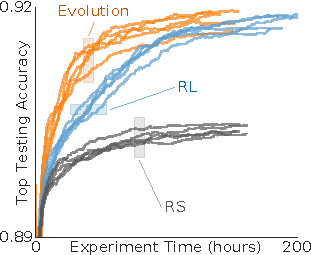
\includegraphics[scale=0.8]{AutoKeras_1}
	\end{subfigure}
	\begin{subfigure}{0.3\textwidth}
		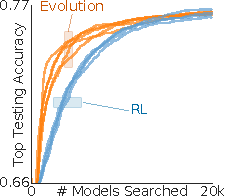
\includegraphics{AutoKeras_2}
	\end{subfigure}
	\begin{subfigure}{0.3\textwidth}
		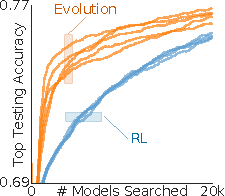
\includegraphics{AutoKeras_3}
	\end{subfigure}
	\caption{Reproduced figures from \citep{Jin2018} demonstrating effective reporting of NAS efficiency}
	\label{fig:reproduce}
\end{figure}

%!TEX root = ../thesis.tex
%*******************************************************************************
%****************************** Third Chapter **********************************
%*******************************************************************************
\chapter{My third chapter}

% **************************** Define Graphics Path **************************
\ifpdf
    \graphicspath{{Chapter3/Figs/Raster/}{Chapter3/Figs/PDF/}{Chapter3/Figs/}}
\else
    \graphicspath{{Chapter3/Figs/Vector/}{Chapter3/Figs/}}
\fi
%!TEX root = ../thesis.tex
%*******************************************************************************
%*********************************** Fith Chapter *****************************
%*******************************************************************************

\chapter{Experiments}

\ifpdf
    \graphicspath{{Chapter5/Figs/Raster/}{Chapter5/Figs/PDF/}{Chapter5/Figs/}}
\else
    \graphicspath{{Chapter5/Figs/Vector/}{Chapter5/Figs/}}
\fi

\section{Investigation into the effects of various hyperparameters on the performance of BNNs on simple problems} \label{sec:hypparam}

There has been little systematic study into how the various hyper-parameters of a Bayesian Neural Network affect the final performance of network. This set of experiments aims to characterise the performance of small BNNs on a range of regression tasks while varying a number of hyper-parameters, in an attempt to extract trends.

The form of network used is an MLP network, with a number of hidden layers and a number of hidden units in each layer. The priors placed on the weights of the network are multivariate independent Gaussians with zero mean. The width of the priors is varied in experiments. The variational distributions used are independent Gaussains. The data is whitened before training by normalising the data to have 0 mean and a standard deviation of 1. They are optimised with the ADAM optimiser, with the settings learning rate=0.001, \( \beta_1 \)=0.9, \( \beta_2 \)=0.999, \( \epsilon \)=1e-8.

It should be noted that as these are preliminary experiments designed to judge only if there is a worthwhile dependency between the variables investigated and model performance. Multiple seeds were not investigated due to the computational cost. The proximity of points tested is enough to see the variability that affects the final objective metrics of BNN training.

\FloatBarrier
\subsection{Hidden width}

Figure \ref{fig:hidden_width} details the effects of varying the widths of the hidden layers in 2-layer networks with a fixed prior width. There is a clear dependency. Some datasets present with a clear maxima in validation log likelihood with varying layer size, and some reach a maximum level in validation log likelihood and increasing layer width beyond this point has no effect. Intuitively it makes sense for performance to increase as the size of the network increases, the drop-off in performance with even larger layer size is investigated later.

\begin{figure}[p]
	\def\dataset{\bostonvar}
	\def\dataname{\bostonname}
	\begin{subfigure}{0.48\textwidth}
		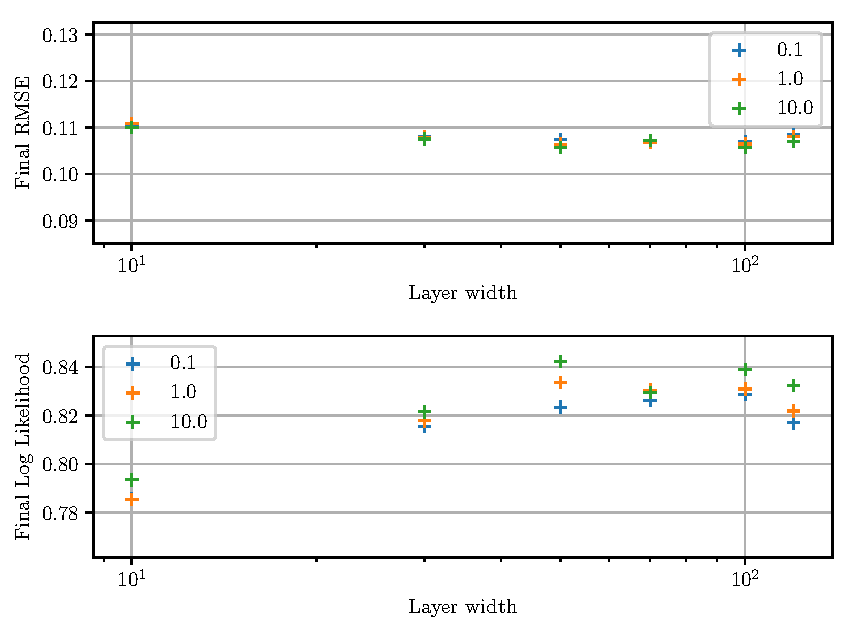
\includegraphics[width=\textwidth]{\dataset/hidden-size}
		\caption{\dataname}
		\label{fig:hidden_width_\dataset}
	\end{subfigure}
	\def\dataset{\concretevar}
	\def\dataname{\concretename}
	\begin{subfigure}{0.48\textwidth}
		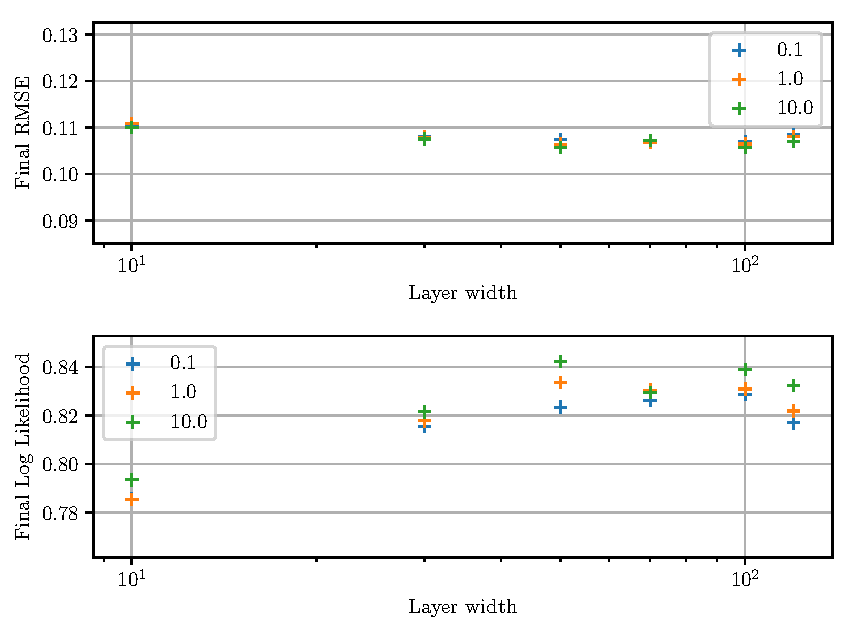
\includegraphics[width=\textwidth]{\dataset/hidden-size}
		\caption{\dataname}
		\label{fig:hidden_width_\dataset}
	\end{subfigure}
	
	\def\dataset{\energyvar}
	\def\dataname{\energyname}
	\begin{subfigure}{0.48\textwidth}
		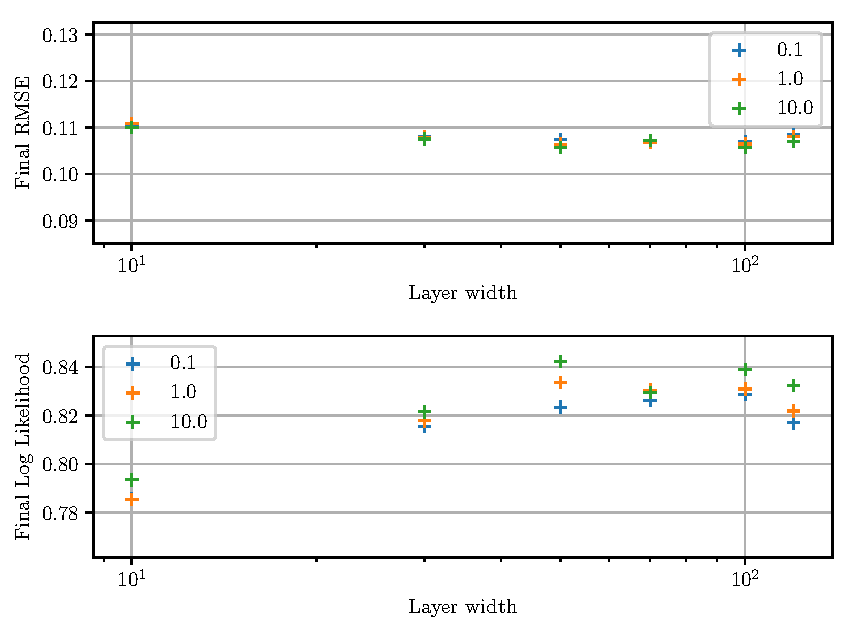
\includegraphics[width=\textwidth]{\dataset/hidden-size}
		\caption{\dataname}
		\label{fig:hidden_width_\dataset}
	\end{subfigure}
	\def\dataset{\kinvar}
	\def\dataname{\kinname}
	\begin{subfigure}{0.48\textwidth}
		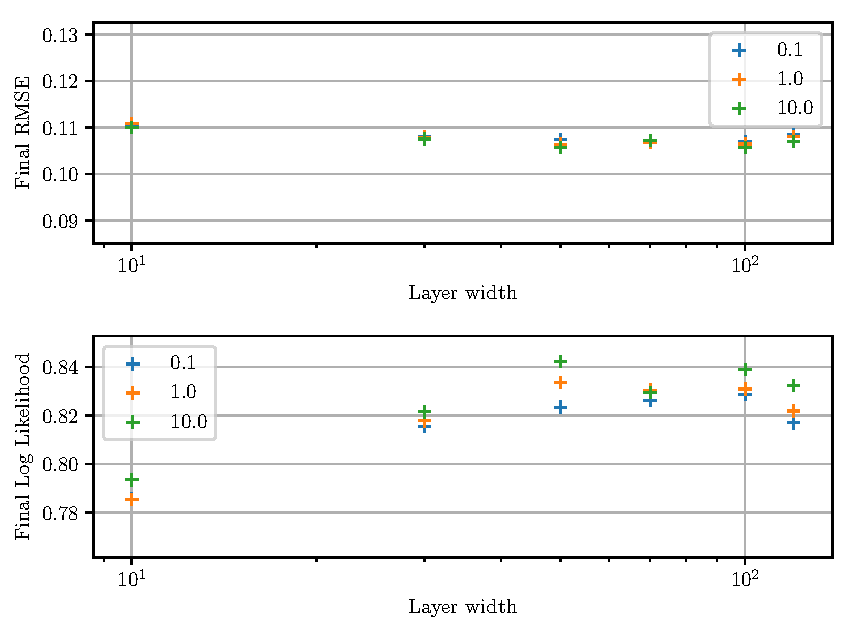
\includegraphics[width=\textwidth]{\dataset/hidden-size}
		\caption{\dataname}
		\label{fig:hidden_width_\dataset}
	\end{subfigure}

	\def\dataset{\powervar}
	\def\dataname{\powername}
	\begin{subfigure}{0.48\textwidth}
		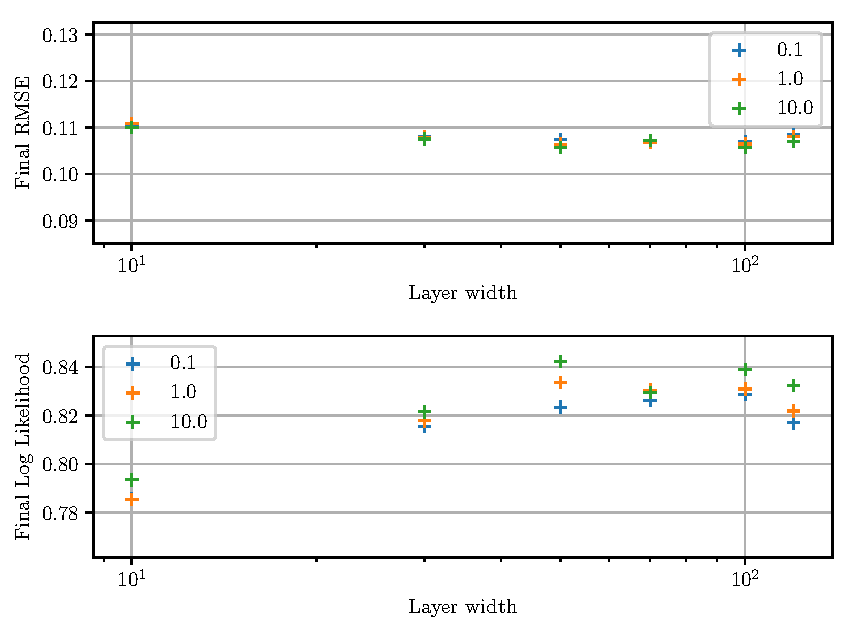
\includegraphics[width=\textwidth]{\dataset/hidden-size}
		\caption{\dataname}
		\label{fig:hidden_width_\dataset}
	\end{subfigure}
	\def\dataset{\proteinvar}
	\def\dataname{\proteinname}
	\begin{subfigure}{0.48\textwidth}
		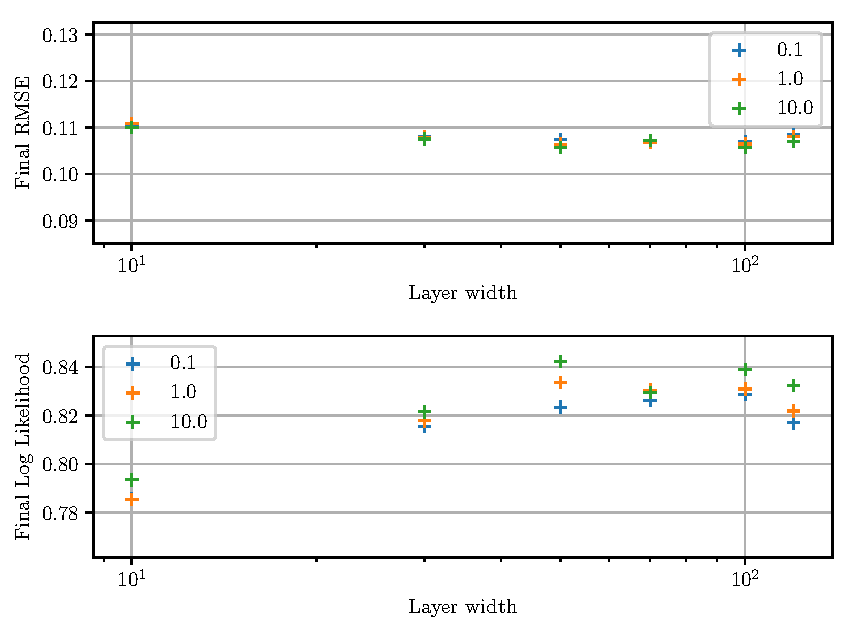
\includegraphics[width=\textwidth]{\dataset/hidden-size}
		\caption{\dataname}
		\label{fig:pruning_\dataset}
	\end{subfigure}
	
	\def\dataset{\winevar}
	\def\dataname{\winename}
	\begin{subfigure}{0.48\textwidth}
		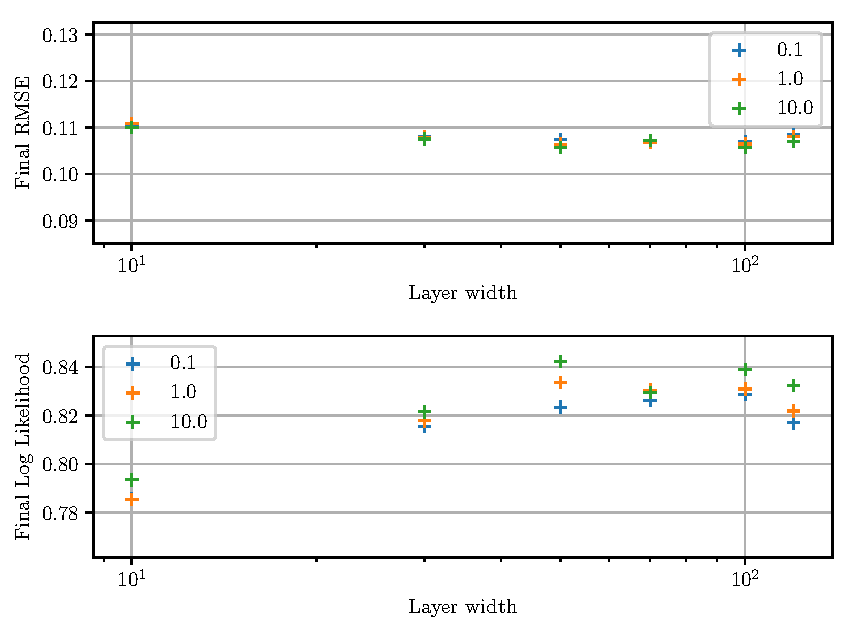
\includegraphics[width=\textwidth]{\dataset/hidden-size}
		\caption{\dataname}
		\label{fig:hidden_width_\dataset}
	\end{subfigure}
	\def\dataset{\yachtnvar}
	\def\dataname{\yachtname}
	\begin{subfigure}{0.48\textwidth}
		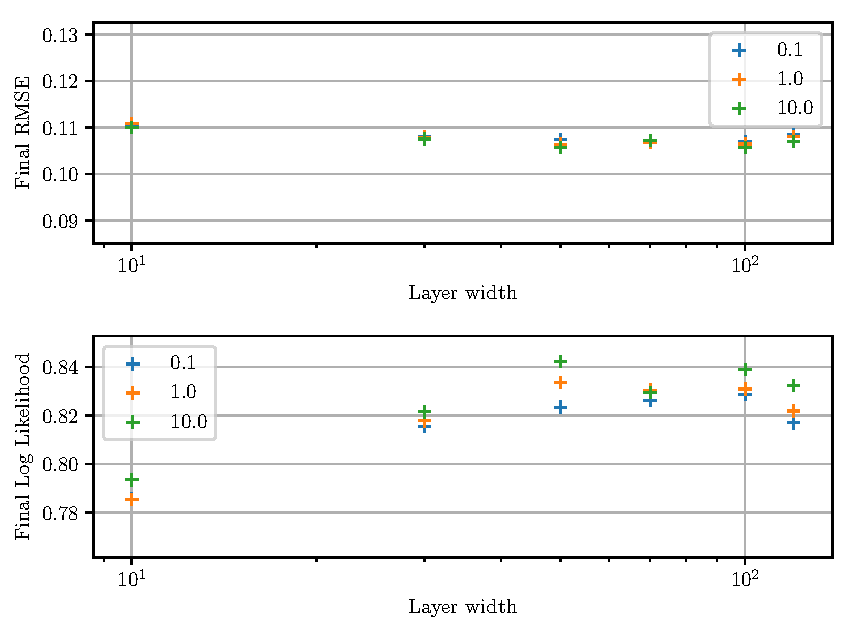
\includegraphics[width=\textwidth]{\dataset/hidden-size}
		\caption{\dataname}
		\label{fig:hidden_width_\dataset}
	\end{subfigure}

	\caption{Final validation log likelihood and RMSE error of various sizes of the hidden layers in 2 layer BNNs. Colour denotes prior width used. Plotted for a number of datasets}
	\label{fig:hidden_width}
\end{figure}

\subsection{Prior width}

Figure \ref{fig:prior_width} details the effects of varying the widths of the prior in 2 layer networks with a fixed architecture. There is again a clear dependency here. For some, the prior width appears to be important up to a particular width, after which it is makes no difference if the width is increased. For some, there is a minor drop off in performance with too large prior width. The clearest trend is that too small a prior width causes significant detriment to performance. This is to be expected. Too small a prior width will over-penalise weights of the size required to produce the required outputs, significantly hampering the model's predictive performance. 

\begin{figure}[p]
	\def\dataset{\bostonvar}
	\def\dataname{\bostonname}
	\begin{subfigure}{0.48\textwidth}
		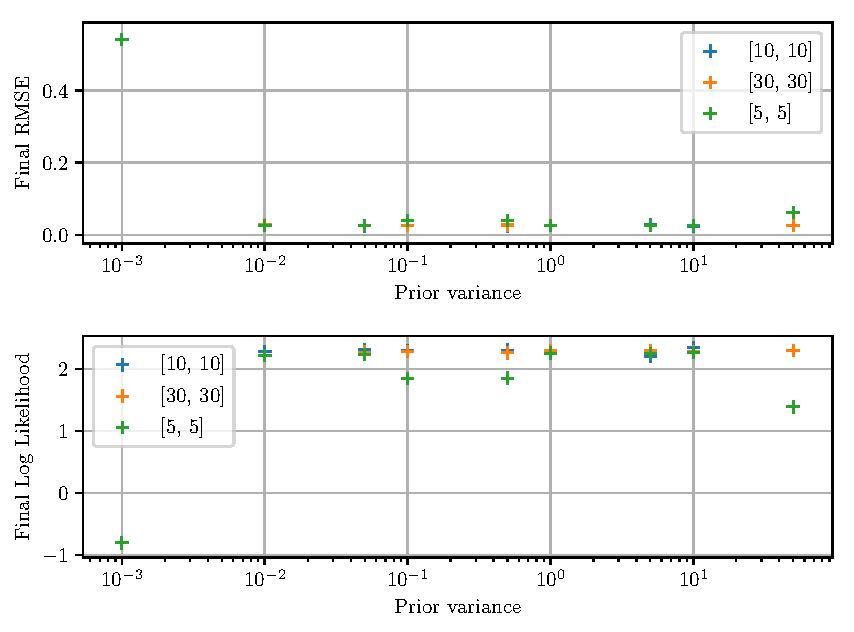
\includegraphics[width=\textwidth]{\dataset/prior-width}
		\caption{\dataname}
		\label{fig:prior_width_\dataset}
	\end{subfigure}
	\def\dataset{\concretevar}
	\def\dataname{\concretename}
	\begin{subfigure}{0.48\textwidth}
		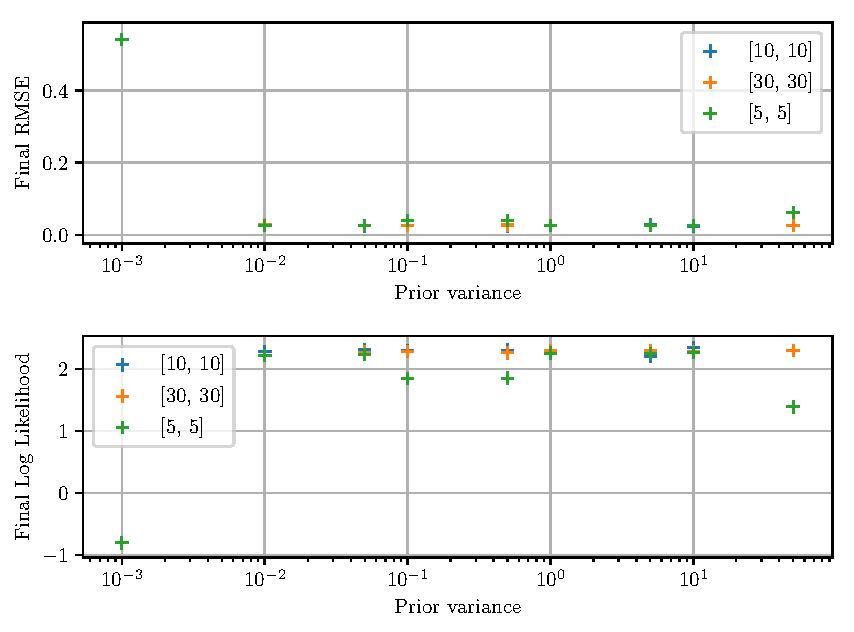
\includegraphics[width=\textwidth]{\dataset/prior-width}
		\caption{\dataname}
		\label{fig:prior_width_\dataset}
	\end{subfigure}

	\def\dataset{\energyvar}
	\def\dataname{\energyname}
	\begin{subfigure}{0.48\textwidth}
		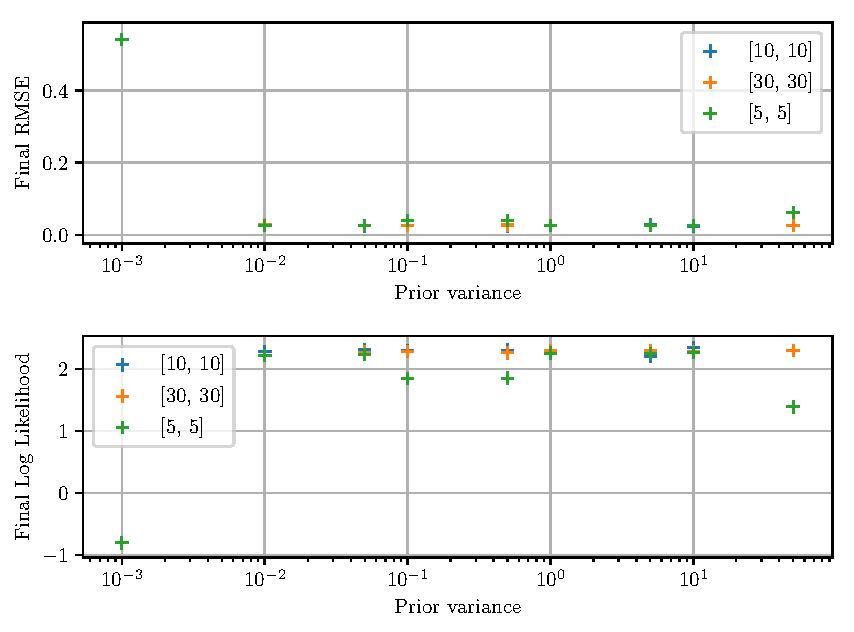
\includegraphics[width=\textwidth]{\dataset/prior-width}
		\caption{\dataname}
		\label{fig:prior_width_\dataset}
	\end{subfigure}
	\def\dataset{\kinvar}
	\def\dataname{\kinname}
	\begin{subfigure}{0.48\textwidth}
		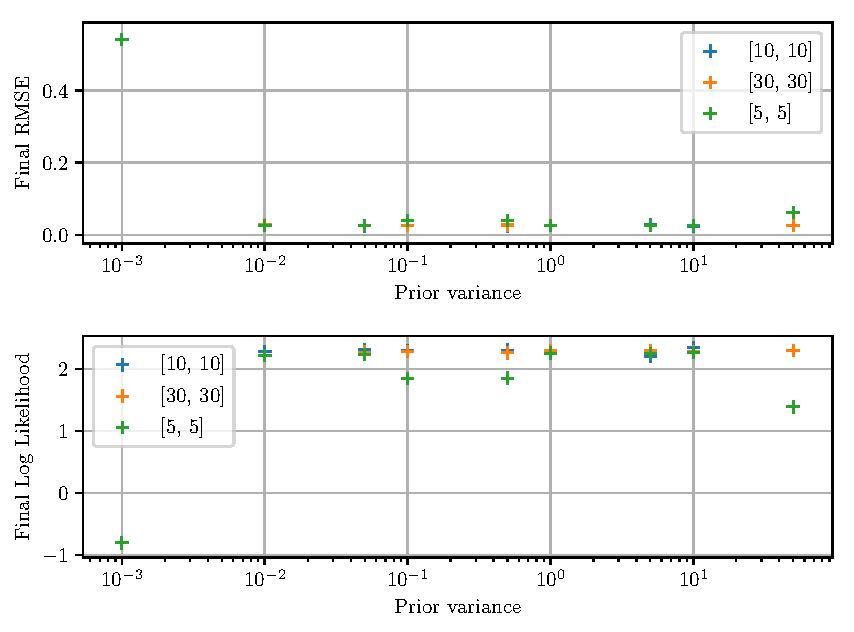
\includegraphics[width=\textwidth]{\dataset/prior-width}
		\caption{\dataname}
		\label{fig:prior_width_\dataset}
	\end{subfigure}
	
	\def\dataset{\powervar}
	\def\dataname{\powername}
	\begin{subfigure}{0.48\textwidth}
		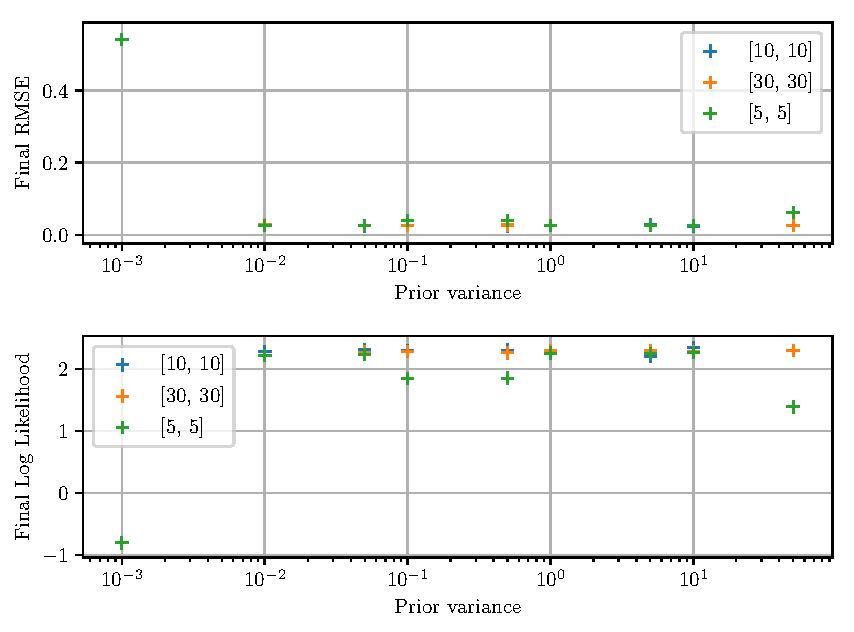
\includegraphics[width=\textwidth]{\dataset/prior-width}
		\caption{\dataname}
		\label{fig:prior_width_\dataset}
	\end{subfigure}
	\def\dataset{\proteinvar}
	\def\dataname{\proteinname}
	\begin{subfigure}{0.48\textwidth}
		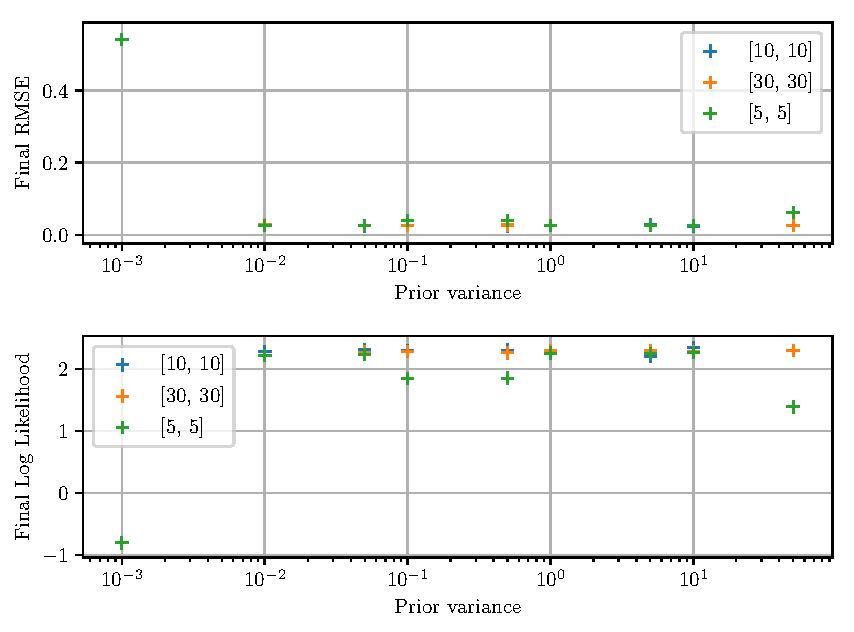
\includegraphics[width=\textwidth]{\dataset/prior-width}
		\caption{\dataname}
		\label{fig:prior_width_\dataset}
	\end{subfigure}
	
	\def\dataset{\winevar}
	\def\dataname{\winename}
	\begin{subfigure}{0.48\textwidth}
		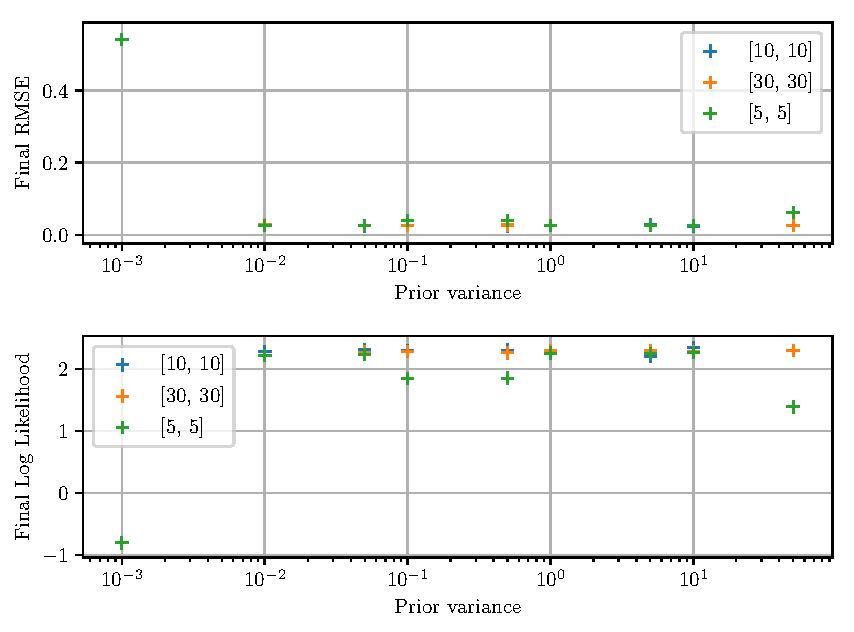
\includegraphics[width=\textwidth]{\dataset/prior-width}
		\caption{\dataname}
		\label{fig:prior_width_\dataset}
	\end{subfigure}
	\def\dataset{\yachtnvar}
	\def\dataname{\yachtname}
	\begin{subfigure}{0.48\textwidth}
		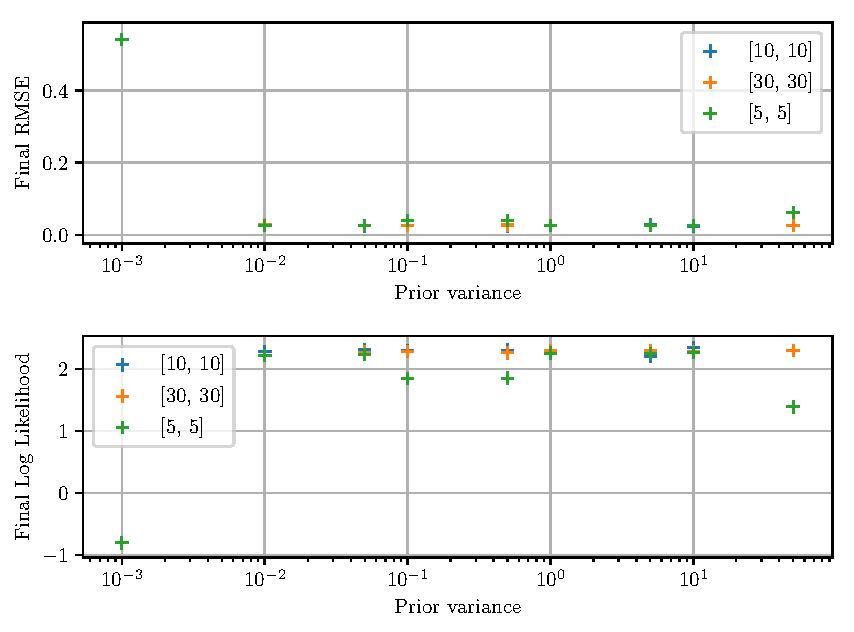
\includegraphics[width=\textwidth]{\dataset/prior-width}
		\caption{\dataname}
		\label{fig:prior_width_\dataset}
	\end{subfigure}
	
	\caption{Final validation log likelihood and RMSE error of various prior widths in 2 layer BNNs. Colour denotes network structure. Plotted for a number of datasets}
	\label{fig:prior_width}
\end{figure}

\subsection{Initialisation of \( \sigma_y^2 \)}

The final parameter investigated in this manner is the initial homoeoskedastic noise on the output of the network, \( y \sim \mathcal{N}(f_\mu(\mathbf{x}), \sigma_y^2) \). Initialisation of this parameter appeared to have little effect on the final performance of the network. There was some effect on the convergence rate of the network. Generally larger \( \sigma_y \) converged faster, but this trend wasn't conclusive. Given the lack of effect on the final performance of the network, it is omitted from the architecture search.

\section{Data Augmentation to control over-fitting and under-fitting}
\label{sec:dataaug}

\begin{figure}[t]
	\begin{subfigure}{0.48\textwidth}
		\def\dataset{\bostonvar}
		\def\dataname{\bostonname}
		\centering
		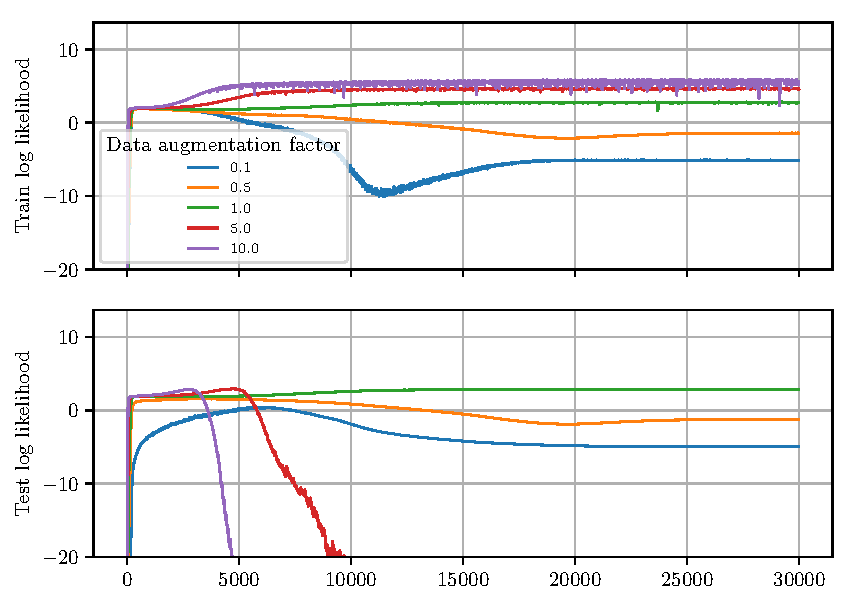
\includegraphics[width=\textwidth]{\dataset/data-multiply-combined}
		\caption{\dataname}
		\label{fig:data_multiply_\dataset}
	\end{subfigure}
%	\begin{subfigure}{0.48\textwidth}
%		\def\dataset{\concretevar}
%		\def\dataname{\concretename}
%		\centering
%		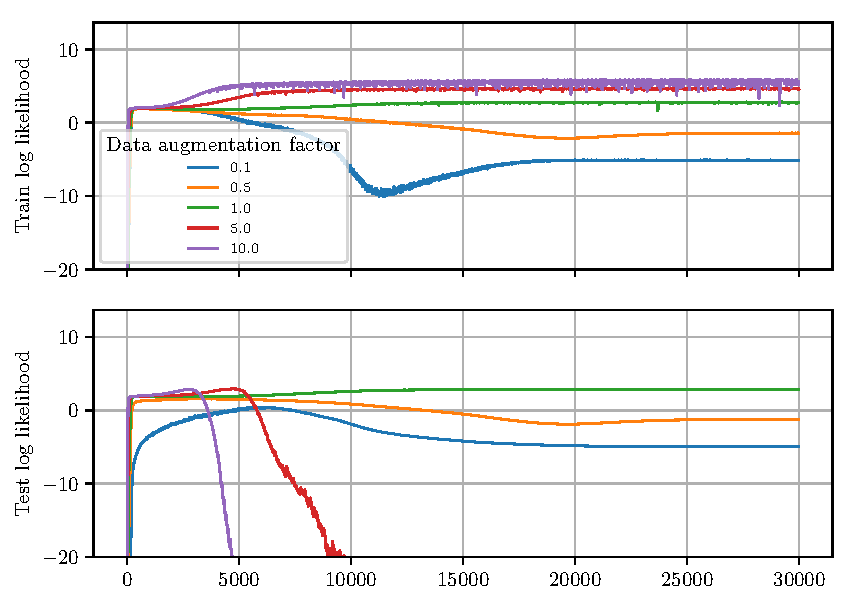
\includegraphics[width=\textwidth]{\dataset/data-multiply-combined}
%		\caption{\dataname}
%		\label{fig:data_multiply_\dataset}
%	\end{subfigure}
%	
	\begin{subfigure}{0.48\textwidth}
		\def\dataset{\energyvar}
		\def\dataname{\energyname}
		\centering
		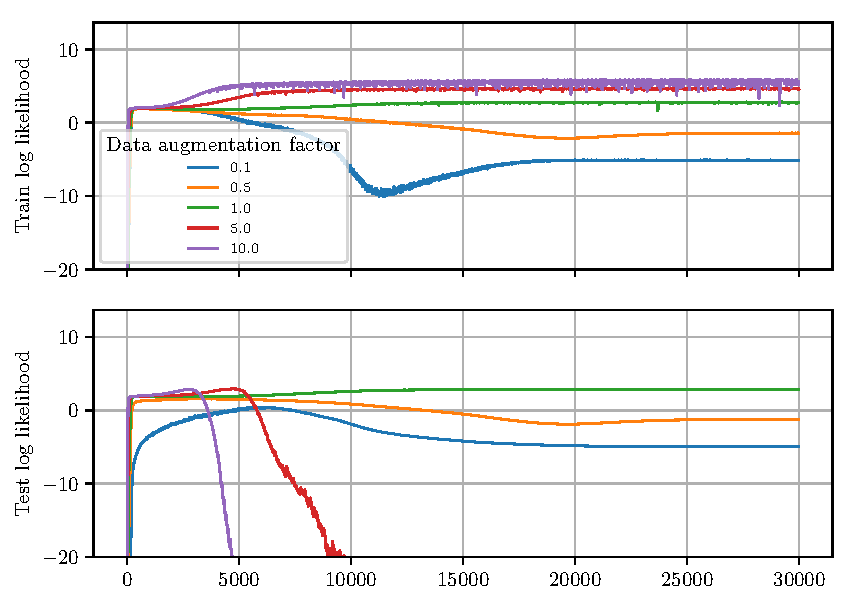
\includegraphics[width=\textwidth]{\dataset/data-multiply-combined}
		\caption{\dataname}
		\label{fig:data_multiply_\dataset}
	\end{subfigure}
%	\begin{subfigure}{0.48\textwidth}
%		\def\dataset{\kinvar}
%		\def\dataname{\kinname}
%		\centering
%		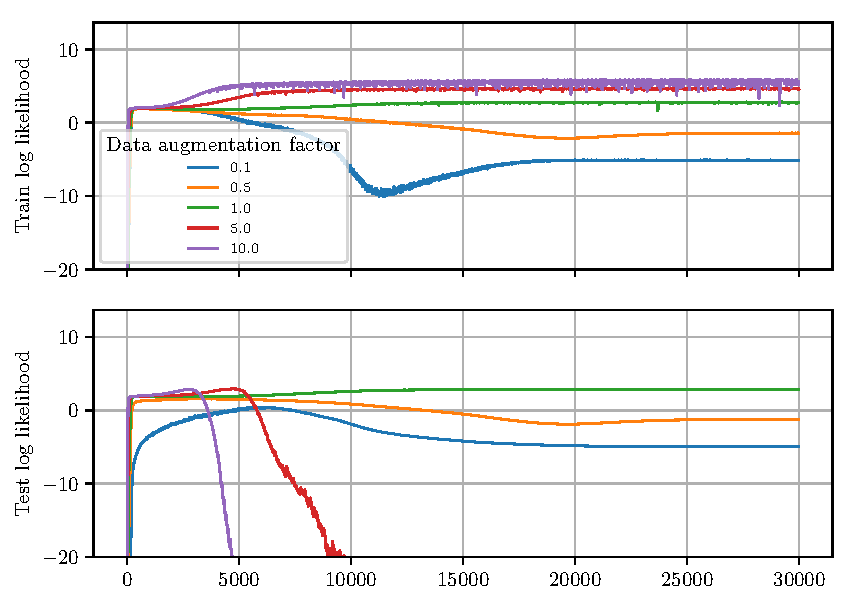
\includegraphics[width=\textwidth]{\dataset/data-multiply-combined}
%		\caption{\dataname}
%		\label{fig:data_multiply_\dataset}
%	\end{subfigure}
%	
%	\begin{subfigure}{0.48\textwidth}
%		\def\dataset{\powervar}
%		\def\dataname{\powername}
%		\centering
%		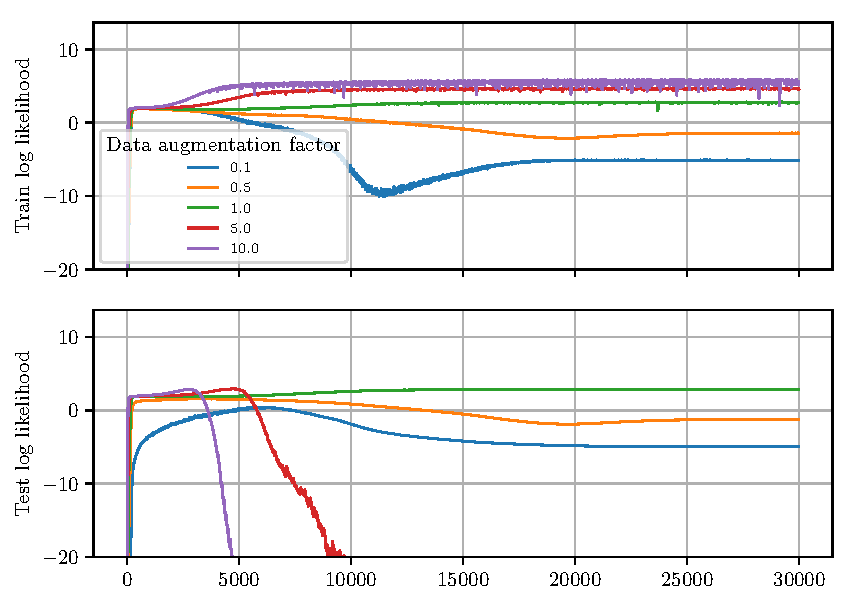
\includegraphics[width=\textwidth]{\dataset/data-multiply-combined}
%		\caption{\dataname}
%		\label{fig:data_multiply_\dataset}
%	\end{subfigure}
%	\begin{subfigure}{0.48\textwidth}
%		\def\dataset{\proteinvar}
%		\def\dataname{\proteinname}
%		\centering
%		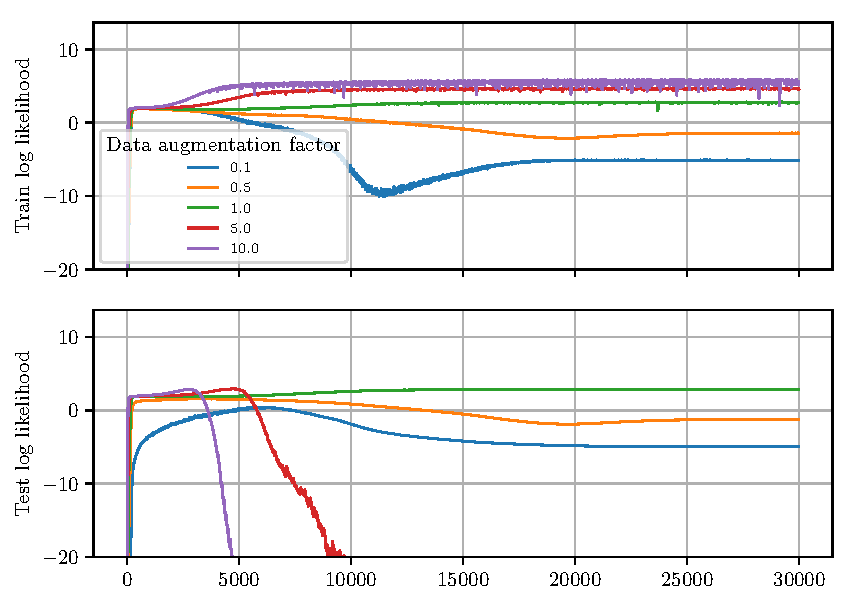
\includegraphics[width=\textwidth]{\dataset/data-multiply-combined}
%		\caption{\dataname}
%		\label{fig:data_multiply_\dataset}
%	\end{subfigure}
%	
	\begin{subfigure}{0.48\textwidth}
		\def\dataset{\winevar}
		\def\dataname{\winename}
		\centering
		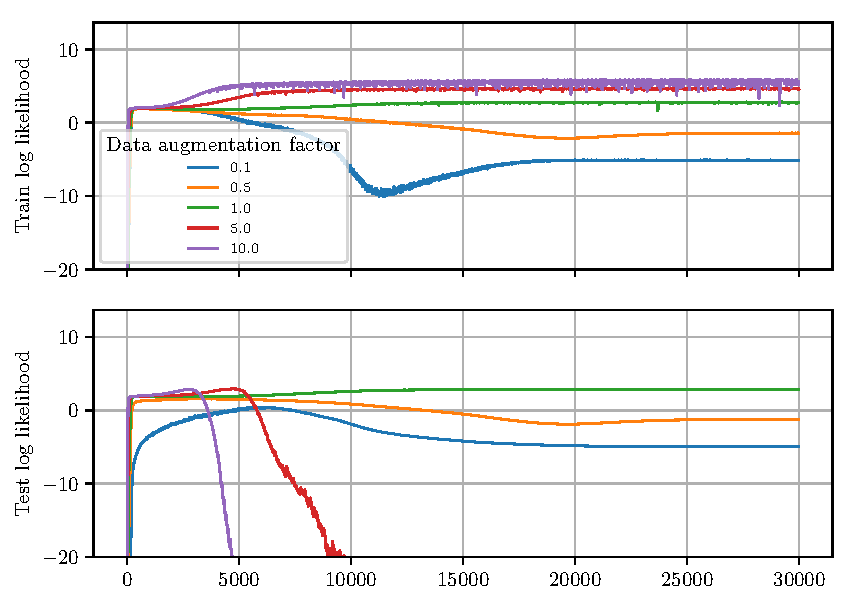
\includegraphics[width=\textwidth]{\dataset/data-multiply-combined}
		\caption{\dataname}
		\label{fig:data_multiply_\dataset}
	\end{subfigure}
	\begin{subfigure}{0.48\textwidth}
		\def\dataset{\yachtnvar}
		\def\dataname{\yachtname}
		\centering
		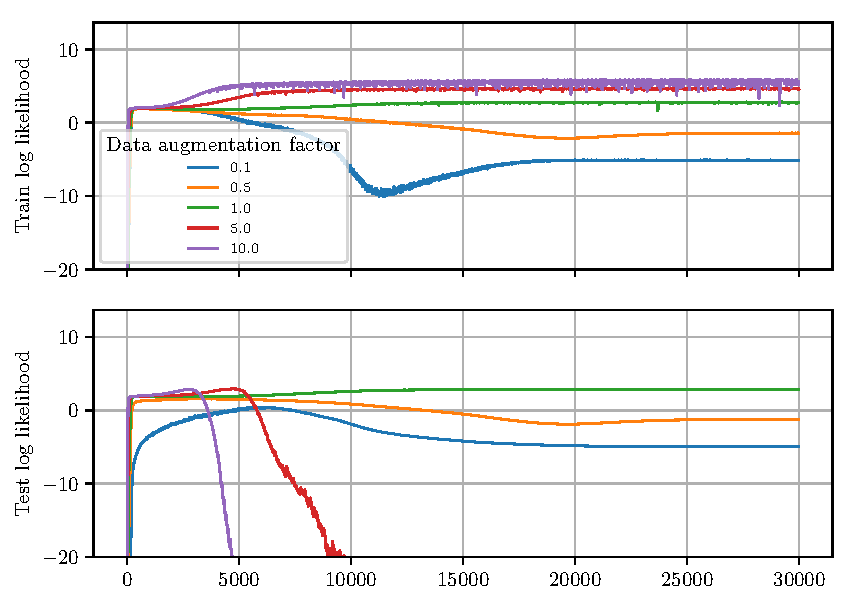
\includegraphics[width=\textwidth]{\dataset/data-multiply-combined}
		\caption{\dataname}
		\label{fig:data_multiply_\dataset}
	\end{subfigure}
	\caption{The effects of modifying the amount of data in a dataset on the train and test log likelihood for a fixed network size. Upper plots show the train set log likelihood through optimisation, and the lower plots the validation log likelihood. With too little,or too much data we see the effects of under-fitting (reduced train and test log likelihood) and over-fitting (increased train log likelihood, significantly decreased test log likelihood) respectively.}
	\label{fig:datamultiply}
\end{figure}

One explanation for the drop-off in performance with larger network size comes from the scaling of the terms in the ELBO cost. The two main terms are the reconstruction loss and the prior fit terms.
\begin{align}
	\ELBO = \underbrace{\E_{q_\phi(\mathbf{w})}\left[ \log P(\mathbf{y} |  \mathbf{w}, \mathbf{x}) \right]}_{\text{reconstruction loss}} - \underbrace{\DKL{q_\phi(\mathbf{w})}{P(\mathbf{w})}}_{\text{prior fit}}
\end{align}
The reconstruction loss is a sum over the log likelihood of the individual data points in the data set, scaling with the quantity of data This term rewards good fit to the data. The prior fit term is a sum over the KL divergence of individual weights (when using a prior with no dependence between weights), therefore scaling with the number of weights in the network. This term rewards keeping the weights close to the prior. 

If we consider a fixed network architecture, we should therefore expect the optimal weights of the network to vary with the amount of data set, as the balance between the two cost terms changes. With a large data-to-network size ratio, we would expect the reconstruction term to overpower the prior fit, resulting in an emphasis on fitting to the train set and potentially over-fitting. With low data-to-network size ratio, we should expect a prioritisation of the prior fit term and a potential for under-fitting. A balance between these terms will give optimal validation set performance. 

In order to test this, the architectures and prior widths that gave optimal performance in the previous experiments were taken. The training datasets were then either under-sampled by some factor by random selection, or over sampled by repeating the dataset and shuffling randomly. The networks were then trained on the new datasets and evaluated on the original validation sets.

Figure \ref{fig:datamultiply} shows the results of these experiments on 4 datasets. We observe the clear signs of under-fitting for low amounts of data - slightly reduced train and validation log likelihood in final performance, and over-fitting with large amounts of data - raised train log likelihood but severely dropped validation log likelihood. We can propose that the under-fitting is likely due to over-regularisation by the KL term and not due to a lack of data by observing that during training, the validation likelihood generally reaches the optimal performance, before being push off from this optima later in training. 

These results help explain the existence of optimal network size being at some finite size, as opposed to an infinite size.

The implications for architecture search are that the size of the network will play a significant role in the performance, in combination with the underlying connective structure. Too large networks will likely systematically under-fit due to over-regularisation by the prior fit term, and small will networks over-fit. 

This does present an interesting method to investigate for restricted size networks, e.g. on embedded devices. Given that for small networks too much data in the training set will cause over-fitting, reducing the amount of data to an empirically appropriate level could see significant performance gains.

\section{Pruning effects in mean-field BNNs}
\label{sec:pruning}

A question raised by the previous section is how the trade-off is being made between the two terms in the ELBO loss, in terms of the weight distributions.

This is investigated by looking at the weights associated with a given hidden unit. Looking at the KL divergence between the weights and the prior, we can investigate how "active" a given weight is. A low KL would indicate that the weight is close to the prior, i.e. close to zero mean and with a width close to the prior, unlikely to be contributing to the performance of the network. A higher KL would indicate the weight is sufficiently dissimilar from the prior. By averaging the KL of all incoming weights to a unit, we can get a measure of the activity of a given neuron. 

The BNNs trained in this experiment utilise the VI training framework with mean field Gaussian priors, utilising Inverse-Gamma hyper-priors on the prior width, with Inverse-Gamma parameters \( \alpha=4.4798, \beta=5.4798 \) (recommended by \citet{wu2018fixing}). They are optimised with the ADAM optimiser, with the settings learning rate=0.001, \( \beta_1 \)=0.9, \( \beta_2 \)=0.999, \( \epsilon \)=1e-8.

Figure \ref{fig:pruning_hist} show example histograms of the distribution of the average KL per neuron. We can clearly see two distinct groups emerge. A larger group, comprising of inactive neurons, and a much smaller group showing the active neurons. Given the very small mean KLs of the weights in the larger group, they are unlikely to contribute significantly to the predictions of the network. We can therefore consider these neurons inactive, or pruned. By placing an appropriate threshold on the value of the average KL for a neuron, we can count the number of total active neurons in a network. 

\begin{figure}
	\centering
	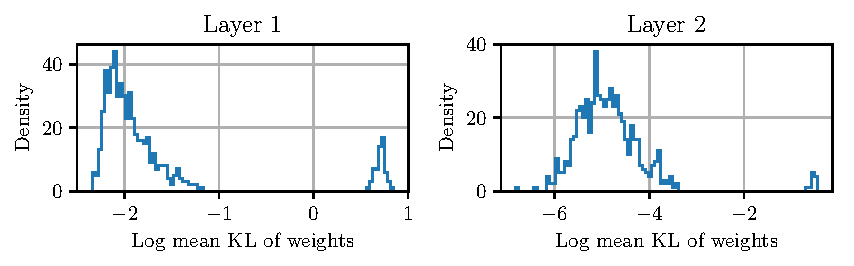
\includegraphics{pruning_example}
	\caption{Histogram of the log mean KL of the weights associated with a give neuron in a 2 layer, 600 unit per layer network trained on the \proteinname \: dataset. Each histogram is for the units of a give layer. Clearly visible is the splitting of the units into two groups, the active and the inactive.}
	\label{fig:pruning_hist}
\end{figure}

Figures \ref{fig:pruning_1} and \ref{fig:pruning_2} detail the results of training various networks on 8 UCI datasets. Networks are defined by a number of layers, and the same hidden width for every layer. Networks of various widths and depths are tested, as appropriate to the specific dataset.

Clearly visible we can see trends in the pruning effect. The number of active neurons increases with network size, utilising all neurons available, up to a point. Past a given break point there is a decreases in the number of neurons effectively utilised. There is a sharp discontinuity in many of these plots in the number of neurons utilised. This comes from the difficulty in exactly defining the boundary of what the threshold is for a neuron to be active. Before this point all neurons are active and so form a single group in the spread of neuron KLs. After this point, two groups exist: the active and inactive. In the transition region between the two, the spread of KL values widens until it separates into the two groups. Defining exactly when to consider neurons inactive is slightly arbitrary, and always leads to the sort of discontinuity seen. 

It is interesting to note that even as fewer neurons become active, in many cases the validation performance of the network continues to increase slightly. This is likely due to the extra regularisation provided by the removal of additional neurons causing the network to generalise better than networks that are slightly smaller. In the limit of large networks, one of two effects appears to present. Either the performance of the network flat-lines, or we see a decrease in performance. The flat-lining behaviour is what we would hope to see in a Bayesian method. For smaller models, adding more units increases the model's capacity to explain the data. Once sufficient capacity is reached, the Bayesian method prunes out the unwanted extra capacity. 

The decrease in performance seen on some datasets is not explained by this interpretation. One theory to explain this is the additional Monte Carlo noise that the pruned units enter into the gradient estimates. While pruned weights have zero mean, they still have a variance and so will likely have some magnitude when sampled. More pruned units will cause more noise. If the optimisation is difficult (i.e. it is a difficult function to learn) it may become increasingly difficult for the optimiser to make headway towards an optimal model in light of noisy gradients, reducing performance. Investigating optimisers other than ADAM may provide more answers.
	
Another point of interest is that these trends tend to match with the width of the network, rather than with the total number of neurons or weights in the network. Further investigation into the pruning in individual layers of the network shows that most active neurons are in the first layer of the network, with significantly fewer in later layers. This would imply that the size of the first layer of the network is the bottle-neck in performance in this case, and that subsequent layers need not be as wide, as per conventional methodology. This is a potential deficiency of the search space  used, with all layers the same size proposed for this project. An alternative to this that attempts to resolve this issue does not change the methodology is proposed earlier.

\begin{figure}[ph]
	\def\dataset{\bostonvar}
	\def\dataname{\bostonname}
	\begin{subfigure}{0.48\textwidth}
		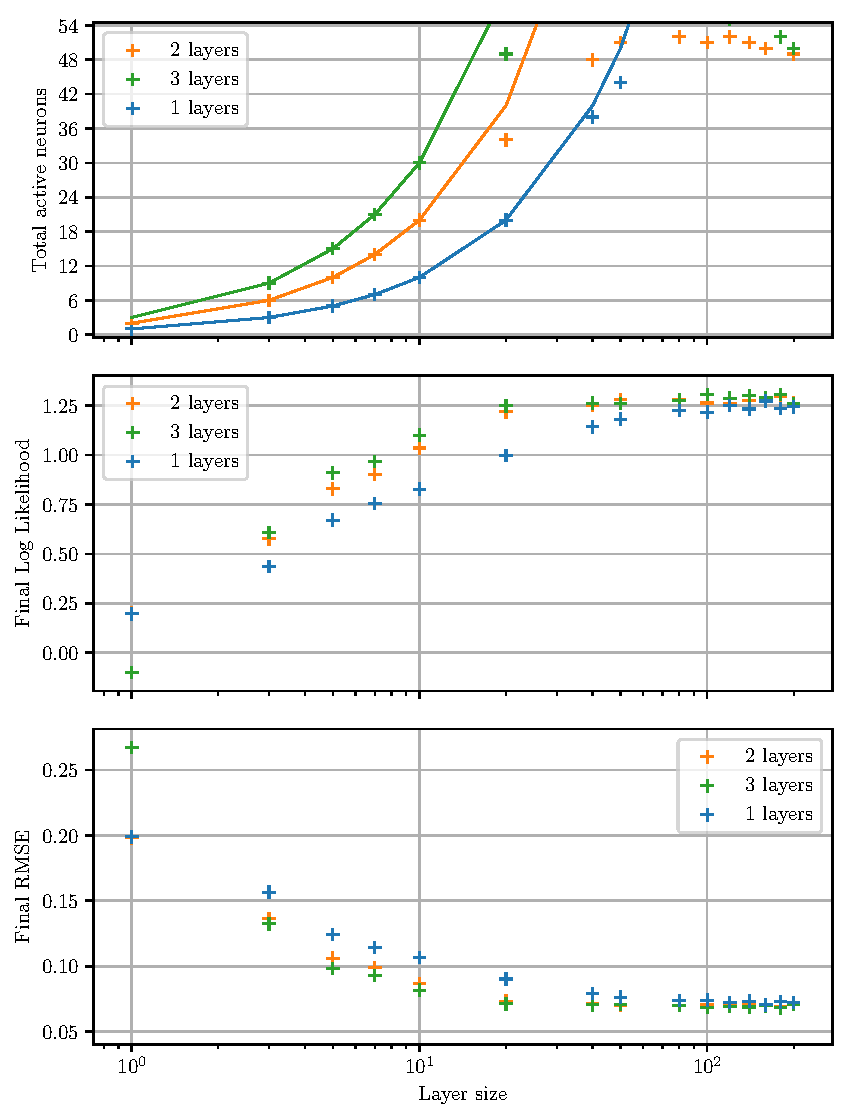
\includegraphics[width=\textwidth]{\dataset/pruning_combined}
		\caption{\dataname}
		\label{fig:pruning_\dataset}
	\end{subfigure}
	\def\dataset{\concretevar}
	\def\dataname{\concretename}
	\begin{subfigure}{0.48\textwidth}
		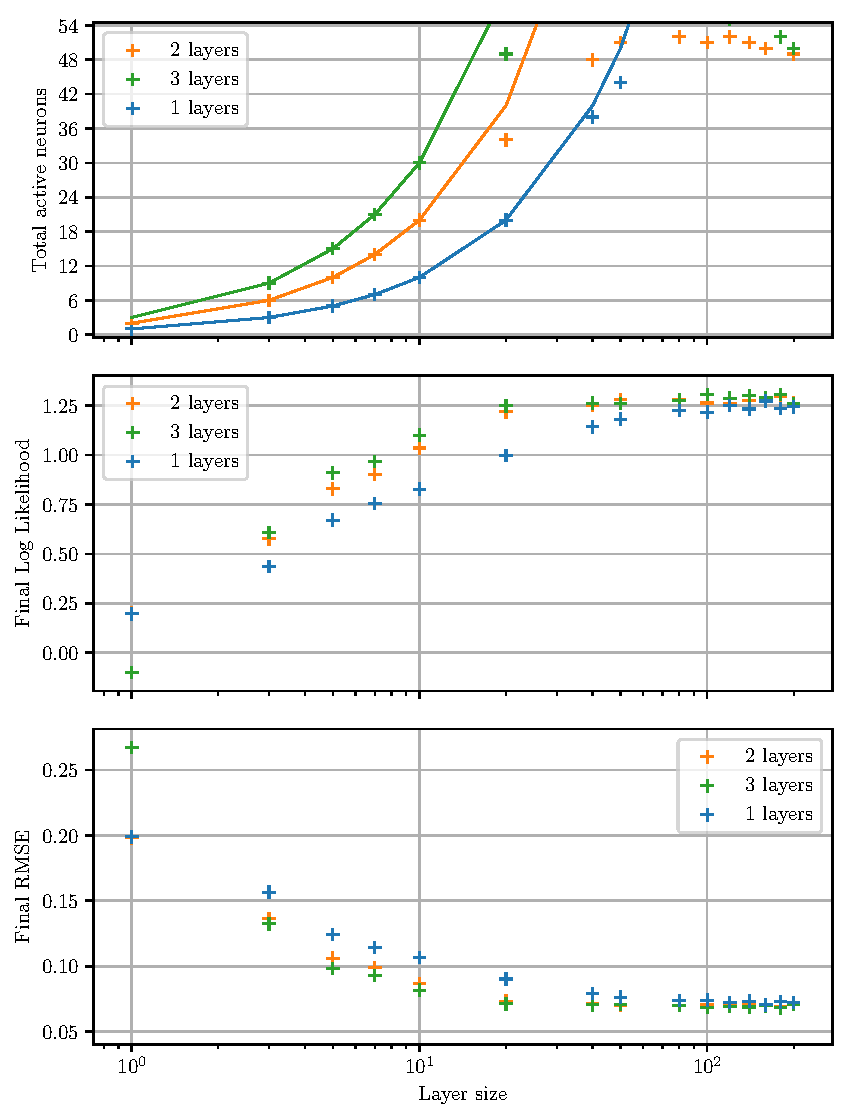
\includegraphics[width=\textwidth]{\dataset/pruning_combined}
		\caption{\dataname}
		\label{fig:pruning_\dataset}
	\end{subfigure}
	
	\def\dataset{\energyvar}
	\def\dataname{\energyname}
	\begin{subfigure}{0.48\textwidth}
		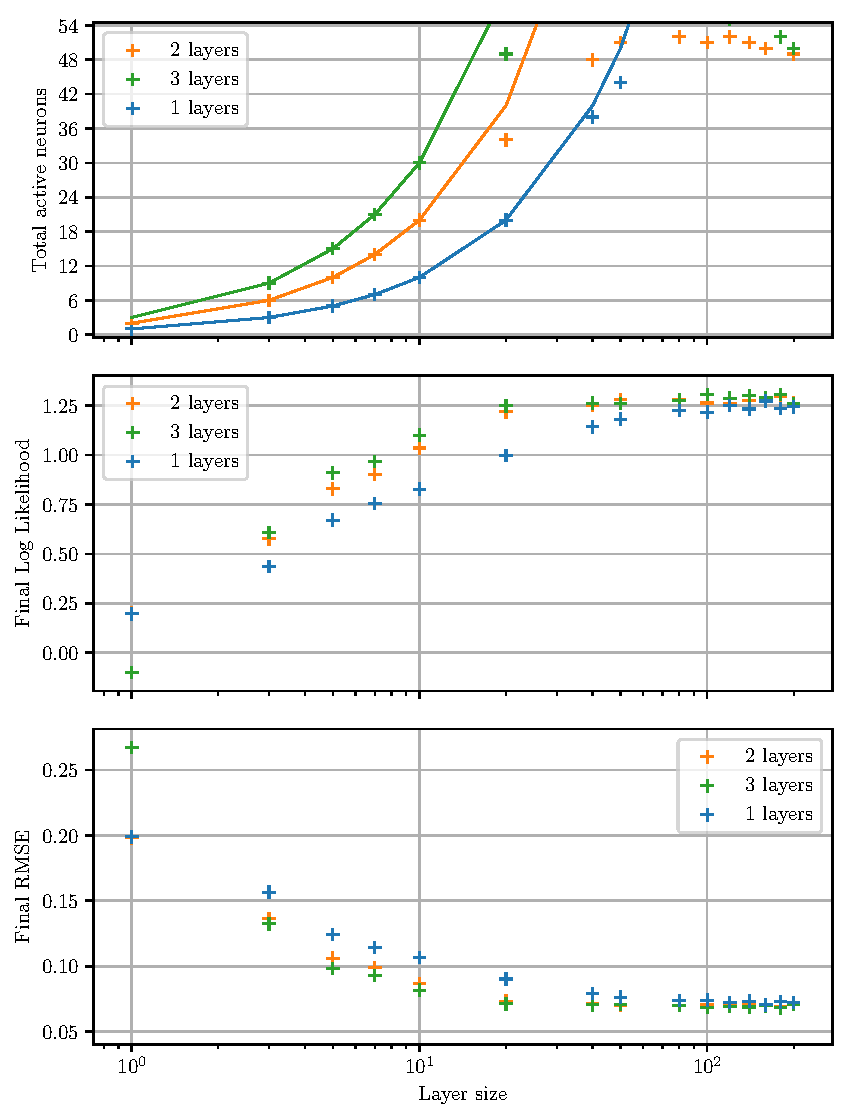
\includegraphics[width=\textwidth]{\dataset/pruning_combined}
		\caption{\dataname}
		\label{fig:pruning_\dataset}
	\end{subfigure}
	\def\dataset{\kinvar}
	\def\dataname{\kinname}
	\begin{subfigure}{0.48\textwidth}
		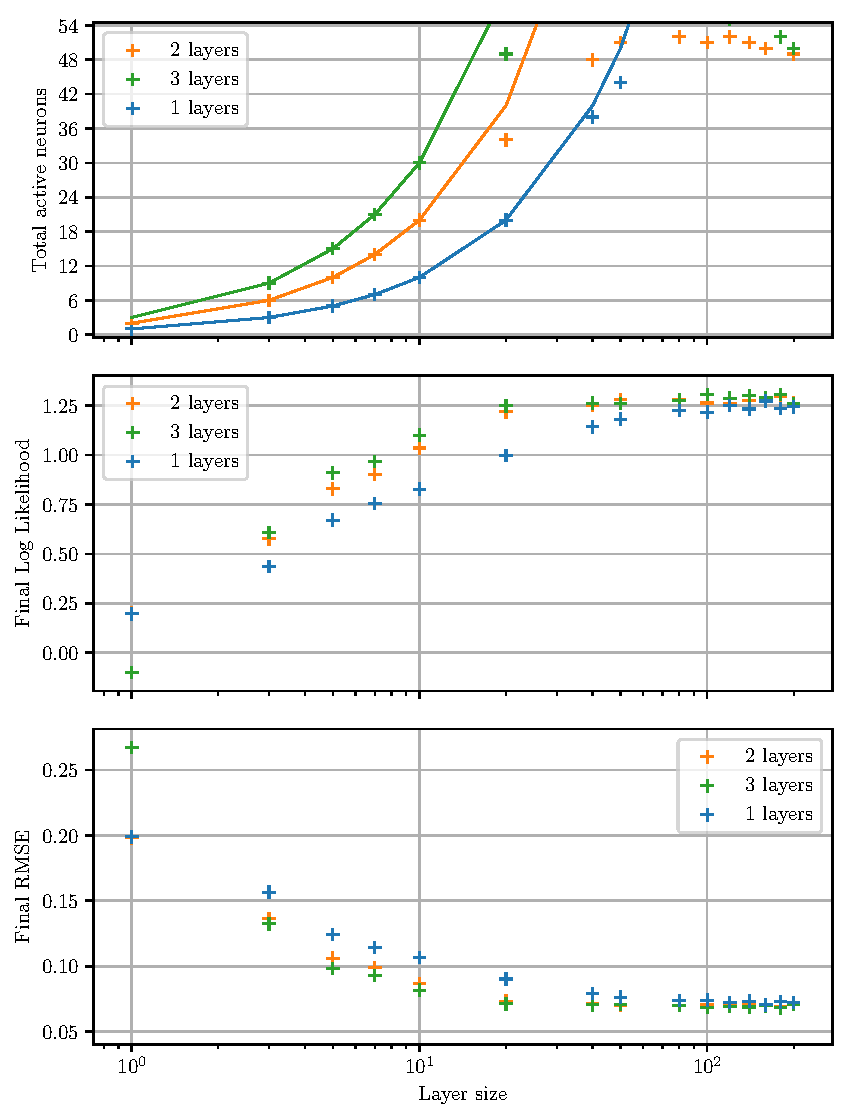
\includegraphics[width=\textwidth]{\dataset/pruning_combined}
		\caption{\dataname}
		\label{fig:pruning_\dataset}
	\end{subfigure}
	\caption{Plots detailing the effect of pruning in VI BNNs on various datasets for a range of architectures. Upper plots show the number of units active in the network, defined by the average KL of units input weights. Solid lines show the total number of units available in the network. Middle plots show the average log likelihood over the last 20 optimisation steps of the network. Lower plots show the average RMSE error over the last 20 optimisation steps of the network. Here we see clearly the effects of model pruning occurring, with the number of active unit in a given model remaining limited with increasing model size. A corresponding effect on performance is seen.}
	\label{fig:pruning_1}
\end{figure}

\begin{figure}[ph]
	\def\dataset{\powervar}
	\def\dataname{\powername}
	\begin{subfigure}{0.48\textwidth}
		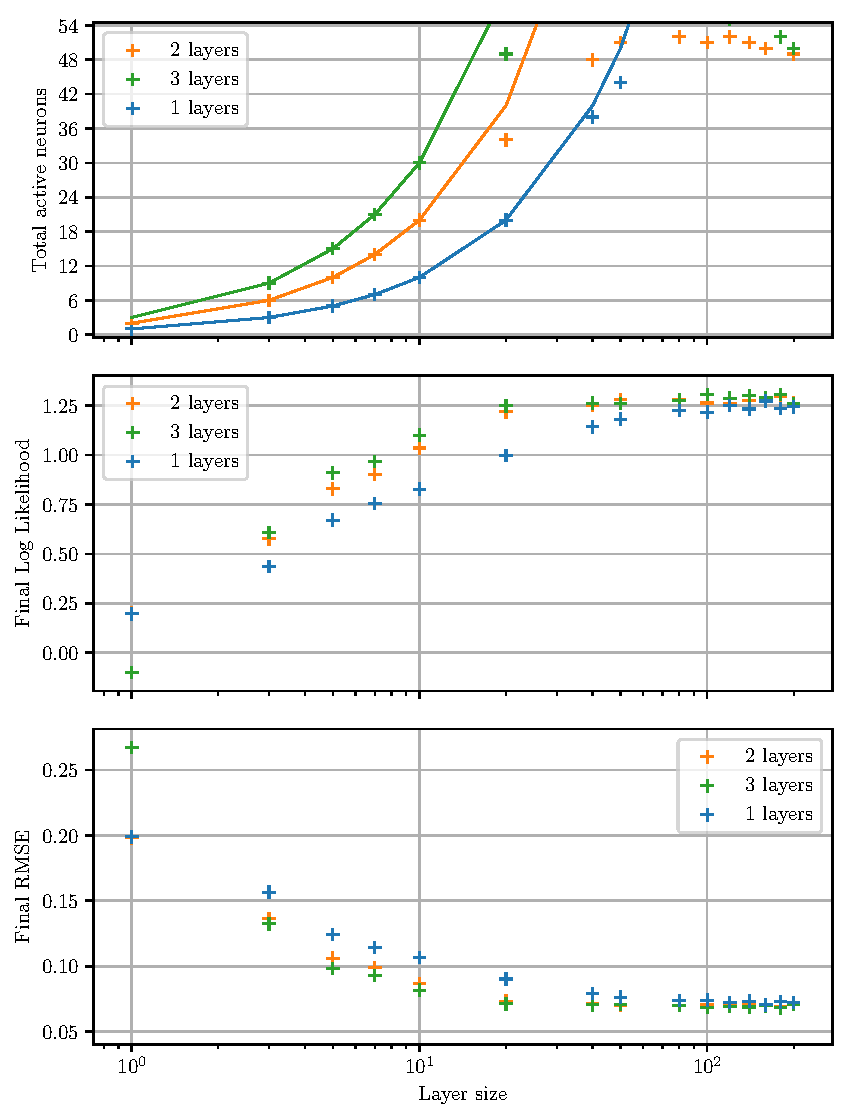
\includegraphics[width=\textwidth]{\dataset/pruning_combined}
		\caption{\dataname}
		\label{fig:pruning_\dataset}
	\end{subfigure}
	\def\dataset{\proteinvar}
	\def\dataname{\proteinname}
	\begin{subfigure}{0.48\textwidth}
		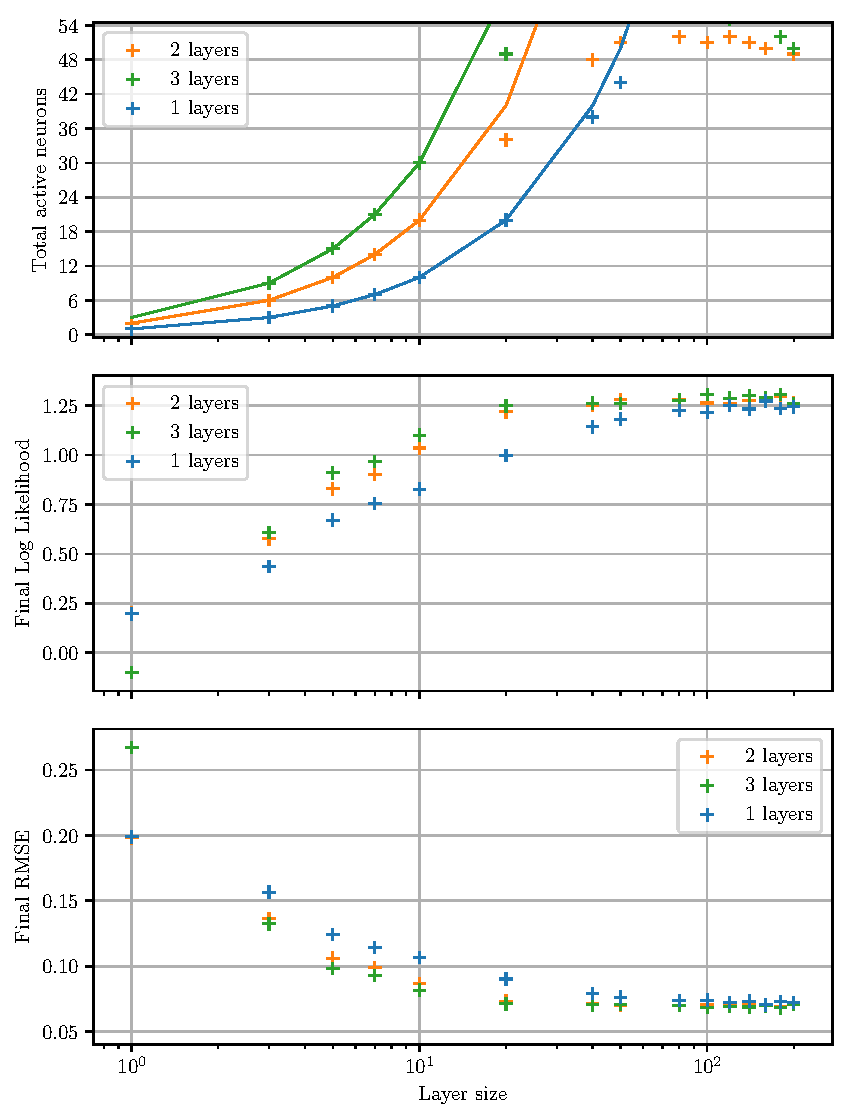
\includegraphics[width=\textwidth]{\dataset/pruning_combined}
		\caption{\dataname}
		\label{fig:pruning_\dataset}
	\end{subfigure}
	
	\def\dataset{\winevar}
	\def\dataname{\winename}
	\begin{subfigure}{0.48\textwidth}
		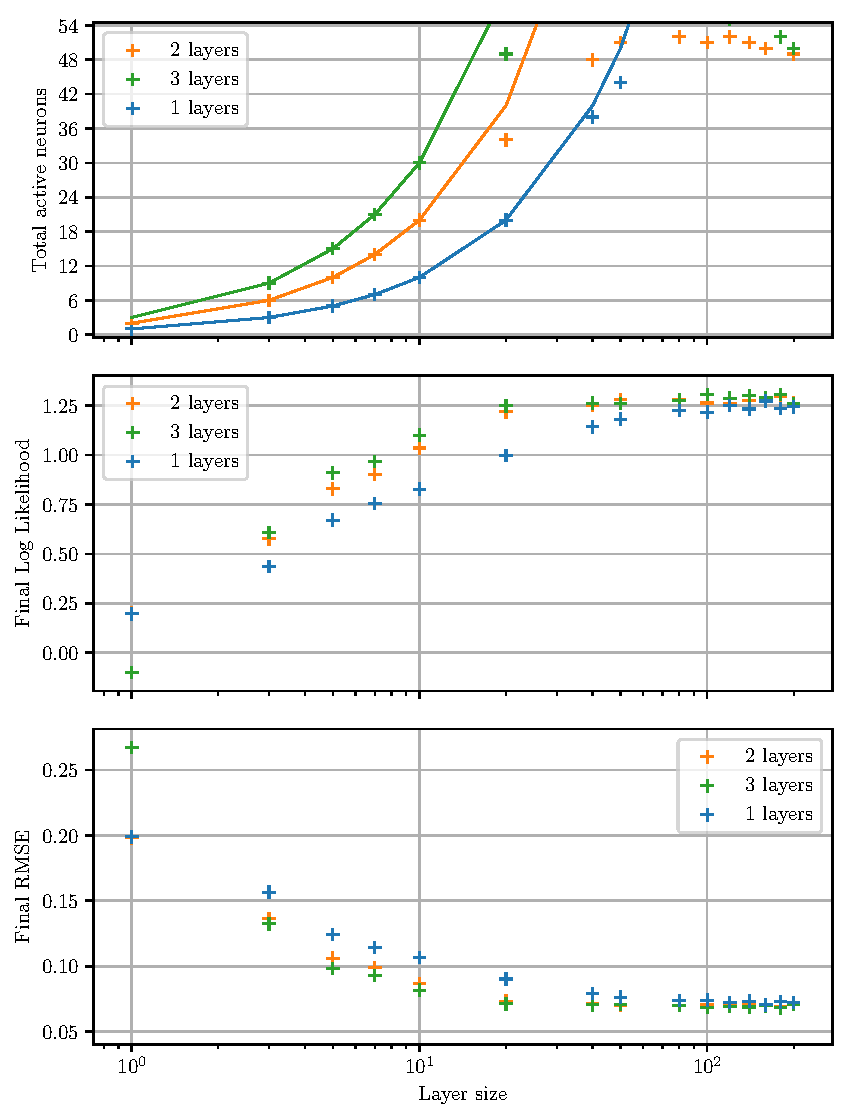
\includegraphics[width=\textwidth]{\dataset/pruning_combined}
		\caption{\dataname}
		\label{fig:pruning_\dataset}
	\end{subfigure}
	\def\dataset{\yachtnvar}
	\def\dataname{\yachtname}
	\begin{subfigure}{0.48\textwidth}
		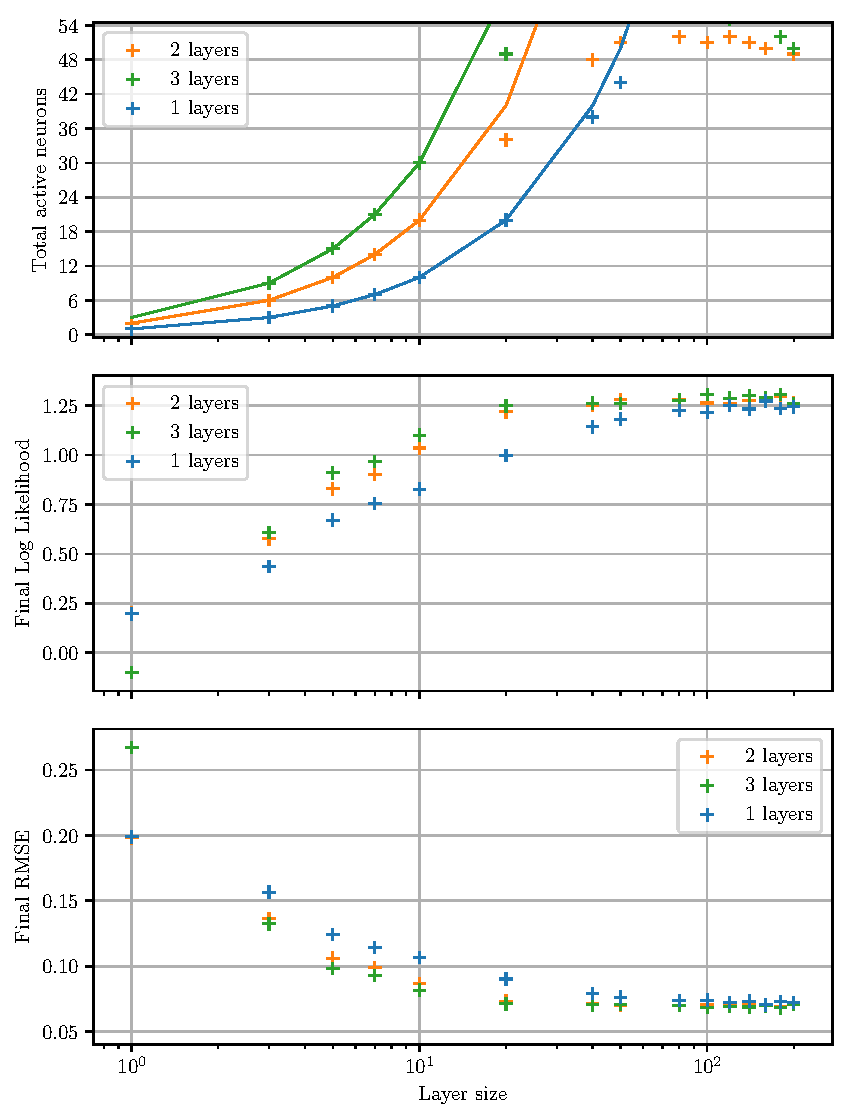
\includegraphics[width=\textwidth]{\dataset/pruning_combined}
		\caption{\dataname}
		\label{fig:pruning_\dataset}
	\end{subfigure}
	\caption{Plots detailing the effect of pruning in VI BNNs on various datasets for a range of architectures. Upper plots show the number of units active in the network, defined by the average KL of units input weights. Solid lines show the total number of units available in the network. Middle plots show the average log likelihood over the last 20 optimisation steps of the network. Lower plots show the average RMSE error over the last 20 optimisation steps of the network. Here we see clearly the effects of model pruning occurring, with the number of active unit in a given model remaining limited with increasing model size. A corresponding effect on performance is seen.}
	\label{fig:pruning_2}
\end{figure}

\section{Empirical kernel and hyper-parameter selection for GPAR models of architecture performance}
\label{sec:model}

Gaussian Process model fitting is a non-trivial task. To do some one must pick appropriate kernels and training hyper-parameters. In the GPAR model there are a number of other considerations, discussed earlier. This section looks to empirically investigate the choice of kernel and hyper-parameters for application to the search space of architecture search. In order to produce a good surrogate model to use in Bayesian Optimisation, it is necessary to find good training setting and kernel choices.

The datasets fitted to are the results of the models trained in the previous section. Three checkpoints are used from the training of the models: 1000 steps, 4000 steps and the final step (typically 30,000-50,000). These points are chosen for two reasons. First from observation the first two points lie in the region where it is not immediately obvious which network will end up with the better performance. Beyond this point models tend to only slowly asymptote to their optima. This makes the modelling task more interesting. Second, it means that the computation saved from early stopping is significant. We only incur the significant additional cost of going from the second output to the final if we believe to to be a good idea in light of the observed training so far. This subset of models define a search space with a discrete set of network deaths and widths over a given range. Each model reported in this section is run on 5 differently selected subsets of data and trained with a different random seed. The results are reported as the mean and standard deviation of results obtained. 

These tests are performed in two sections: investigation into appropriate kernels, and an investigation into the other training settings of the model. It was ensured that the parameters not tested in each experiment were sufficiently good. However, they may not be optimal and so this pair of experiment implicitly assumes that the results of each are reasonably independent of the other settings.

The models are optimised with the L-BFGS-B algorithm, using the implementation from the Python package SciPy.

\subsection{Kernel investigation}

First we investigate the appropriate form of kernel to use. A non-linear EQ kernel is always placed on the input. In addition a combination of some, all, or none of the following are also used, added together: a liner kernel on the inputs \( \mathbf{x} \), a linear kernel on the outputs \( \mathbf{y}_{1:i} \) and a non-linear kernel on the outputs.

Table \ref{tbl:kernel_half} shows the results of fitting these models to a training set of half the dataset, randomly selected. Table \ref{tbl:kernel_small} shows the results of fitting these models to a training set consisting of 10 points from the dataset, randomly selected. Both are then validated on the remaining data and the log likelihood reported. The second table, the low data case, is of particular interest for the architecture search case as we are looking to make good prediction about model performance from just a few samples.

The results of this investigation are inconclusive. When using a large amount of data, there seems to be a preference for using all the possible kernel option, but this still not close to unanimous. In the low data case, the differences in mean are often overshadowed by the standard deviation of the results. The kernel chosen for use in experiments is therefore a non-linear kernel on the inputs and a linear kernel on the outputs as it appears to overall be the best fitting, but this is not completely clear.

\afterpage{%
	\clearpage% Flush earlier floats (otherwise order might not be correct)
	\thispagestyle{empty}% empty page style (?)
	\begin{landscape}
		%\begin{tabular}{lll|rrrrrrr}
		%	\toprule
		%	\multicolumn{3}{c}{Model settings} & \multicolumn{7}{c}{Dataset} \\
		%	Markov length & Input scales tied & Joint trained & bostonHousing & concrete & energy & kin8nm & power-plant & wine-quality-red &   yacht \\
		
		%\begin{tabular}{lll|rrrrrrr}
		%	\toprule
		%	\multicolumn{3}{c}{Kernal settings} & \multicolumn{7}{c}{Dataset} \\\\
		%	\shortstack[l]{Linear kernal\\on inputs} & \shortstack[l]{Linear kernal\\on outputs} & \shortstack[l]{Non-linear kernal\\on outputs} & bostonHousing & concrete & energy & kin8nm & power-plant & wine-quality-red &   yacht \\
		\begin{table}
			\scriptsize
			\begin{tabular}{lll|rrrrrrr}
				\toprule
				\multicolumn{3}{c}{Kernal settings} & \multicolumn{7}{c}{Dataset} \\\\
				\shortstack[l]{Linear kernal\\on inputs} & \shortstack[l]{Linear kernal\\on outputs} & \shortstack[l]{Non-linear kernal\\on outputs} & bostonHousing & concrete & energy & kin8nm & power-plant & wine-quality-red &   yacht \\
				\midrule
				\multirow{4}{*}{False} & \multirow{2}{*}{False} & False &            -2.64 ± 0.351 &  -1.86 ± 0.429 &    -0.649 ± 0.2 &  1.37 ± 0.304 &  -0.437 ± 0.299 &   -0.874 ± 0.246 &    -51 ± 98.7 \\
				&       & True  &            -2.42 ± 0.269 &  -1.75 ± 0.374 &   -0.49 ± 0.211 &  2.87 ± 0.409 &   0.167 ± 0.235 &   -0.554 ± 0.168 &  -48.9 ± 97.7 \\
				\cline{2-10}
				& \multirow{2}{*}{True} & False &            -2.79 ± 0.248 &  -1.82 ± 0.457 &  -0.529 ± 0.222 &    2.97 ± 0.4 &  0.0153 ± 0.245 &   -0.611 ± 0.169 &  -49.1 ± 96.8 \\
				&       & True  &              -2.56 ± 0.3 &  -1.75 ± 0.354 &  -0.391 ± 0.207 &  \textbf{3.12 ± 0.432} &   0.196 ± 0.212 &    -0.57 ± 0.187 &  -52.7 ± 7.68 \\
				\cline{1-10}
				\cline{2-10}
				\multirow{4}{*}{True} & \multirow{2}{*}{False} & False &            -2.64 ± 0.352 &  -1.86 ± 0.429 &  -0.644 ± 0.203 &    1.4 ± 0.31 &  -0.388 ± 0.306 &   -0.797 ± 0.213 &  -50.5 ± 98.3 \\
				&       & True  &            \textbf{-2.41 ± 0.265} &   \textbf{-1.74 ± 0.37} &  -0.489 ± 0.212 &  2.88 ± 0.412 &    0.197 ± 0.26 &    -0.529 ± 0.16 &  -48.7 ± 97.2 \\
				\cline{2-10}
				& \multirow{2}{*}{True} & False &            -2.78 ± 0.303 &  -1.82 ± 0.458 &  -0.527 ± 0.222 &  2.95 ± 0.431 &     0.14 ± 0.13 &     -0.6 ± 0.174 &  -48.7 ± 96.8 \\
				&       & True  &            -2.56 ± 0.284 &   -1.77 ± 0.39 &  \textbf{-0.387 ± 0.208} &    3.1 ± 0.44 &   \textbf{0.245 ± 0.223} &   \textbf{-0.531 ± 0.161} &  \textbf{-48.1 ± 96.9} \\
				\bottomrule
			\end{tabular}
			\caption{The per data-point validation log likelihood of fitting various combinations of kernels to the performance characteristics of BNNs trained on various datasets. Training sets are 50\% of samples randomly selected. Validation set is the remaining data. Each experiment run 5 times with different seeds. The mean and standard deviation of the results are reported.}
			\label{tbl:kernel_half}
		\end{table}
		
		\begin{table}
			\scriptsize
			\begin{tabular}{lll|rrrrrrr}
				\toprule
				\multicolumn{3}{c}{Kernal settings} & \multicolumn{7}{c}{Dataset} \\
				\shortstack[l]{Linear kernal\\on inputs} & \shortstack[l]{Linear kernal\\on outputs} & \shortstack[l]{Non-linear kernal\\on outputs} & bostonHousing & concrete & energy & kin8nm & power-plant & wine-quality-red &   yacht \\
				\midrule
				\multirow{4}{*}{False} & \multirow{2}{*}{False} & False &               -123 ± 242 &  -23.1 ± 25.9 &   -185 ± 386 &  1.49 ± 2.43 &  0.233 ± 2.48 &     -19.9 ± 27.4 &  -3.93E+03 ± 6.83E+03 \\
				&       & True  &               -124 ± 255 &  -22.9 ± 27.3 &  \textbf{-96.6 ± 136} &  3.19 ± 1.25 &   1.27 ± 1.48 &     -19.9 ± 27.8 &  -3.25E+03 ± 5.05E+03 \\
				\cline{2-10}
				& \multirow{2}{*}{True} & False &               -118 ± 234 &  \textbf{-21.2 ± 23.6} &   -580 ± 586 &   2.8 ± 1.37 &   1.37 ± 2.23 &     -33.7 ± 37.9 &  -4.02E+03 ± 6.92E+03 \\
				&       & True  &               -120 ± 241 &  -36.2 ± 32.9 &   -457 ± 451 &  1.11 ± 4.54 &   \textbf{1.71 ± 1.75} &     -33.5 ± 37.9 &  -4.24E+03 ± 7.37E+03 \\
				\cline{1-10}
				\cline{2-10}
				\multirow{4}{*}{True} & \multirow{2}{*}{False} & False &               -123 ± 241 &      -23 ± 26 &   -169 ± 350 &   1.1 ± 2.12 &   0.53 ± 1.96 &     -19.8 ± 27.4 &   -3.92E+03 ± 6.8E+03 \\
				&       & True  &               \textbf{-105 ± 210} &    -24 ± 29.3 &   -144 ± 207 &  2.78 ± 1.47 &    1.31 ± 1.5 &     -19.7 ± 27.9 &  \textbf{-3.18E+03 ± 5.09E+03} \\
				\cline{2-10}
				& \multirow{2}{*}{True} & False &               -121 ± 242 &  -21.3 ± 24.4 &   -379 ± 531 &  2.97 ± 1.35 &   1.34 ± 2.21 &     -19.8 ± 27.4 &     -4E+03 ± 6.88E+03 \\
				&       & True  &               -120 ± 243 &  -24.6 ± 24.6 &   -210 ± 296 &  \textbf{3.22 ± 1.14} &   1.63 ± 1.57 &     \textbf{-19.6 ± 27.8} &  -4.14E+03 ± 7.16E+03 \\
				\bottomrule
			\end{tabular}
			\caption{The per data-point validation log likelihood of fitting various combinations of kernels to the performance characteristics of BNNs trained on various datasets. Training sets are 10 samples randomly selected. Validation set is the remaining data. Each experiment run 5 times with different seeds. The mean and standard deviation of the results are reported.}
			\label{tbl:kernel_small}
		\end{table}
		
		\clearpage
		
		\begin{table}
			\scriptsize
			\begin{tabular}{lll|rrrrrrr}
				\toprule
				\multicolumn{3}{c}{Model settings} & \multicolumn{7}{c}{Dataset} \\
				Markov length & Input scales tied & Joint trained & bostonHousing & concrete & energy & kin8nm & power-plant & wine-quality-red &   yacht \\
				\midrule
				\multirow{4}{*}{False} & \multirow{2}{*}{False} & False &            -2.64 ± 0.351 &  -1.86 ± 0.429 &    -0.649 ± 0.2 &  1.37 ± 0.304 &  -0.437 ± 0.299 &   -0.874 ± 0.246 &    -51 ± 98.7 \\
				&       & True  &            \textbf{-2.42 ± 0.269} &  \textbf{-1.75 ± 0.374} &   -0.49 ± 0.211 &  2.87 ± 0.409 &   0.167 ± 0.235 &   -0.554 ± 0.168 &  -48.9 ± 97.7 \\
				\cline{2-10}
				& \multirow{2}{*}{True} & False &            -2.79 ± 0.248 &  -1.82 ± 0.457 &  -0.529 ± 0.222 &    2.97 ± 0.4 &  0.0153 ± 0.245 &   -0.611 ± 0.169 &  -49.1 ± 96.8 \\
				&       & True  &              -2.56 ± 0.3 &  \textbf{-1.75 ± 0.354} &  \textbf{-0.391 ± 0.207} &  \textbf{3.12 ± 0.432} &   0.196 ± 0.212 &    -0.57 ± 0.187 &  -5.27 ± 7.68 \\
				\cline{1-10}
				\cline{2-10}
				\multirow{4}{*}{True} & \multirow{2}{*}{False} & False &            -2.64 ± 0.352 &  -1.86 ± 0.429 &  -0.644 ± 0.203 &    1.4 ± 0.31 &  -0.388 ± 0.306 &   -0.797 ± 0.213 &  -50.5 ± 98.3 \\
				&       & True  &            \textbf{-2.41 ± 0.265} &   \textbf{-1.74 ± 0.37} &  -0.489 ± 0.212 &  2.88 ± 0.412 &    0.197 ± 0.26 &    \textbf{-0.529 ± 0.16} &  -48.7 ± 97.2 \\
				\cline{2-10}
				& \multirow{2}{*}{True} & False &            -2.78 ± 0.303 &  -1.82 ± 0.458 &  -0.527 ± 0.222 &  2.95 ± 0.431 &     0.14 ± 0.13 &     -0.6 ± 0.174 &  -48.7 ± 96.8 \\
				&       & True  &            -2.56 ± 0.284 &   -1.77 ± 0.39 &  -0.387 ± 0.208 &    \textbf{3.1 ± 0.44} &   \textbf{0.245 ± 0.223} &   \textbf{-0.531 ± 0.161} &  -48.1 ± 96.9 \\
				\bottomrule
			\end{tabular}
			\caption{The per data-point validation log likelihood of fitting various combinations of model hyper-parameter to the performance characteristics of BNNs trained on various datasets. Training sets are 50\% of the samples randomly selected. Validation set is the remaining data. Each experiment run 5 times with different seeds. The mean and standard deviation of the results are reported.}
			\label{tbl:hyp_half}
		\end{table}
		
		\begin{table}		
			\scriptsize
			\begin{tabular}{lll|rrrrrrr}
				\toprule
				\multicolumn{3}{c}{Model settings} & \multicolumn{7}{c}{Dataset} \\
				Markov length & Input scales tied & Joint trained & bostonHousing & concrete & energy & kin8nm & power-plant & wine-quality-red &   yacht \\
				\midrule
				\multirow{4}{*}{False} & \multirow{2}{*}{False} & False &               -123 ± 242 &  -23.1 ± 25.9 &   -185 ± 386 &  1.49 ± 2.43 &  0.233 ± 2.48 &     -19.9 ± 27.4 &  -3.93E+03 ± 6.83E+03 \\
				&       & True  &               -124 ± 255 &  -22.9 ± 27.3 &  -96.6 ± 136 &  3.19 ± 1.25 &   1.27 ± 1.48 &     -19.9 ± 27.8 &  -3.25E+03 ± 5.05E+03 \\
				\cline{2-10}
				& \multirow{2}{*}{True} & False &               -118 ± 234 &  -21.2 ± 23.6 &   -580 ± 586 &   2.8 ± 1.37 &   1.37 ± 2.23 &     -33.7 ± 37.9 &  -4.02E+03 ± 6.92E+03 \\
				&       & True  &               -120 ± 241 &  -36.2 ± 32.9 &   -457 ± 451 &  1.11 ± 4.54 &   1.71 ± 1.75 &     -33.5 ± 37.9 &  -4.24E+03 ± 7.37E+03 \\
				\cline{1-10}
				\cline{2-10}
				\multirow{4}{*}{True} & \multirow{2}{*}{False} & False &               -123 ± 241 &      -23 ± 26 &   -169 ± 350 &   1.1 ± 2.12 &   0.53 ± 1.96 &     -19.8 ± 27.4 &   -3.92E+03 ± 6.8E+03 \\
				&       & True  &               -105 ± 210 &    -24 ± 29.3 &   -144 ± 207 &  2.78 ± 1.47 &    1.31 ± 1.5 &     -19.7 ± 27.9 &  -3.18E+03 ± 5.09E+03 \\
				\cline{2-10}
				& \multirow{2}{*}{True} & False &               -121 ± 242 &  -21.3 ± 24.4 &   -379 ± 531 &  2.97 ± 1.35 &   1.34 ± 2.21 &     -19.8 ± 27.4 &     -4E+03 ± 6.88E+03 \\
				&       & True  &               -120 ± 243 &  -24.6 ± 24.6 &   -210 ± 296 &  3.22 ± 1.14 &   1.63 ± 1.57 &     -19.6 ± 27.8 &  -4.14E+03 ± 7.16E+03 \\
				\bottomrule
			\end{tabular}
			\caption{The per data-point validation log likelihood of fitting various combinations of model hyper-parameter to the performance characteristics of BNNs trained on various datasets. Training sets are 10 samples randomly selected. Validation set is the remaining data. Each experiment run 5 times with different seeds. The mean and standard deviation of the results are reported.}
			\label{tbl:hyp_small}		
		\end{table}
	\end{landscape}
	\clearpage% Flush page
}

\subsection{Model fitting hyper-parameters}

We now look at the additional properties of the GPAR model that can be applied. These are described in more depth in the methodology section.
\begin{itemize}
	\item \textbf{Markov structure.} This can be varied from no structure, down to a Markov length of 1.
	\item \textbf{Tying input scales} This can either be active or inactive.
	\item  \textbf{Joint training} This can either be active or not.
\end{itemize}

The results here are again inconclusive. No set of settings appears to be particularly dominant although the one trend that does appear - as one might expect - is that performing joint optimisation is better than not. In the low data case it also appear that tying the scales of the kernels on the input helps. Overall a Markov length of 1 was chosen, as it speeds up training, and the input scales were tied with joint optimisation of the log likelihood performed.

\section{Architecture search experiments} 
\label{sec:archsearch}

The results of section \ref{sec:model} specify the parameters of the surrogate model to be used in the Bayesian Optimisation procedure, and the results from section \ref{sec:pruning} define a search space to be search over. Given the cost of training BNNs, instead of performing these search in an online fashion, the results from section \ref{sec:pruning} are used as a surrogate dataset for training new BNNs. To sample an architecture, the algorithm draws the corresponding results from the pre-trained results. While this may introduce some bias into the results due to only a single random dataset being used, there are no better options due to the cost of training BNNs on the limited resources available.

All results in this section are run on 16 different random seeds to provide a good statistical estimate for the properties of each combination of settings.

To analyse the results of these searches, progression of the searches are measured in terms of the number points in the search space that have been sampled. On the upper plots, the y-axes are the mean best final log likelihood found so far across multiple runs, with a confidence bound. On the other lower plots are the standard deviation of these best results found.

There are two things to look for in these plots when evaluating methods. Final performance, and efficiency of performance. The final performance can be seen by looking at the performance of models at the end of search, the far right of the plots. Higher mean log likelihood, and lower standard deviation is better. The efficiency can be seen by looking at how the mean and standard deviation of the best results progresses through time. Some methods may eventually find good architectures, but take significantly more samples to do so. Higher and further left in mean is better, lower and further left better for the standard deviation.

\subsection{Multi-output search}

The data used here are 3 outputs taken at 1,000, 4,000, and 30,000 or 50,000 optimisation steps (dataset dependant, the final output) from the results of section \ref{sec:pruning}. Each value is the average of the previous 20 optimisation steps results to smooth the noise in objective function that appears in BNN training.

Four search methods are run on this search space. Three Bayesian Optimisation GPAR methods, using the Expected Improvement, Probability of Improvement and Upper Confidence Bound utility functions. The final search method is Random Search as an ablative baseline. At each iteration, the algorithm picks 4 new points to investigate, in the random search case fully training the network, and in the case of the GPAR models, advancing the training by one output stage. 4 choices were used to speed up the algorithm, as sampling a single point at a time proved too slow to run. 

Also investigated in these plots are the effects of deliberately under-sampling when estimating the posterior of the Gaussian Process function. Since multiple points are being tested at each iteration, we want to diversify the points selected, else it is likely we will end up testing multiple points in a very similar location at the maxima of the true acquisition function. By using small, independent sets of samples drawn from the model to estimate the posterior function, we hope to inject some stochastic noise into the acquisition function, spreading out the points sampled among a group of the best options. 

The results of these searches are seen on the left figures \ref{fig:searches_bostonHousing} - \ref{fig:searches_yacht}. In general the results of these searches are promising. After the initial random search, the GPAR methods is more efficient than random search, both in terms of the mean best value found, and the standard deviation of the best value found, implying that the GPAR methods also more consistently find better solutions than random search.

In two cases however, we see that random search outperforms Bayesian optimisation methods. First, on the \bostonname\: set, EI is competitive, but random search pulls ahead further into the search. An explanation from this comes from re-examining the figures \ref{fig:pruning_1}. We see that the results of BNN training are significantly more noisy than in other problems (e.g. in the \bostonname \: problem). This excessive noise on the data will make model fitting and therefore guided optimisation more difficult.

Second, on \yachtname. Looking at figure \ref{fig:pruning_2} again provides an explanation. The majority of points in the dataset have very similar performance. Any difference is likely induced by a small amount of noise in the training. There is therefore very little to be gained here by trying to model this, leading to random search being competitive.

The effect of different acquisitions functions is also not completely clear. Generally, the UCB acquisition function performs worse than EI or PI, with these two competing for best. 

Under-sampling to inject noise into the acquisition function seems to be ineffective. The differences in performance are small, and inconsistent in improving or worsening results. A different method to do parallel Bayesian Optimisation should be investigated.

\subsection{Comparison to final performance only search}

The GPAR model proposed here is reasonably complex. One way of reducing the complexity in order to see if this additional complexity is useful is to model only the final performance of the BNNs, and perform Bayesian Optimisation over this instead. This alternative method is instigated in the same way as the GPAR method.  The right hand plots of \ref{fig:searches_bostonHousing} - \ref{fig:searches_yacht} show the results of this kind of search. 

The x-axes on these plots should be noted. In the 3-output GPAR case, a point is one advancement of training of a network. In the final-performance-only method, it is the training of a complete network. Thus a single point in the final performance modelling case is on average 3 times more expensive to evaluate. The plots of random search are identical in both plots, providing an easy comparison point.

The results show that on 2 tasks the GPAR method outperforms the standard Bayesian Optimisation method, on 3 it is matched within standard error, and worse on 3 .

One explanation for this behaviour could be attributed to the GPAR method "dithering" on model selection in some cases. If the observations of model performance are significantly noisy, this can cause shifts in the maxima of the acquisition function at each time step. As the GPAR method only advances training one step at a time, if this causes it to keep sampling new architectures, it is unlikely to advance a model to completion. Models not advanced to completion cannot be counted as the best architecture found. This would therefore slow down the GPAR method as it will be likely to train many models a step or two, and few to completion, compared to the final-performance-only or random search methods which will train all sampled models to completion. This would be especially likely on noisy dataset, i.e \bostonname \: and \yachtname, and this is what we see.

In some cases this dithering may be beneficial, giving the model a greater amount of exploration and may explain the GPAR method outperforming standard Bayesian Optimisation in 2 cases.

In general the GPAR method is slower to get started, possibly due to the "dithering" reason discussed above, but finds better solutions faster after an initial "burn in" period. The exact cause of when the full GPAR search is better than final performance search is unclear. Further investigation into this is necessary.

By the end of the search however, both models usually find equally good models, whereas random search does not.

%\subsection{Synthetic data}
%Put fig here!!!
%\begin{figure}[h]
%	\def\dataset{synthetic}
%	\def\dataname{Synthetic}
%	\begin{subfigure}{0.48\textwidth}
%		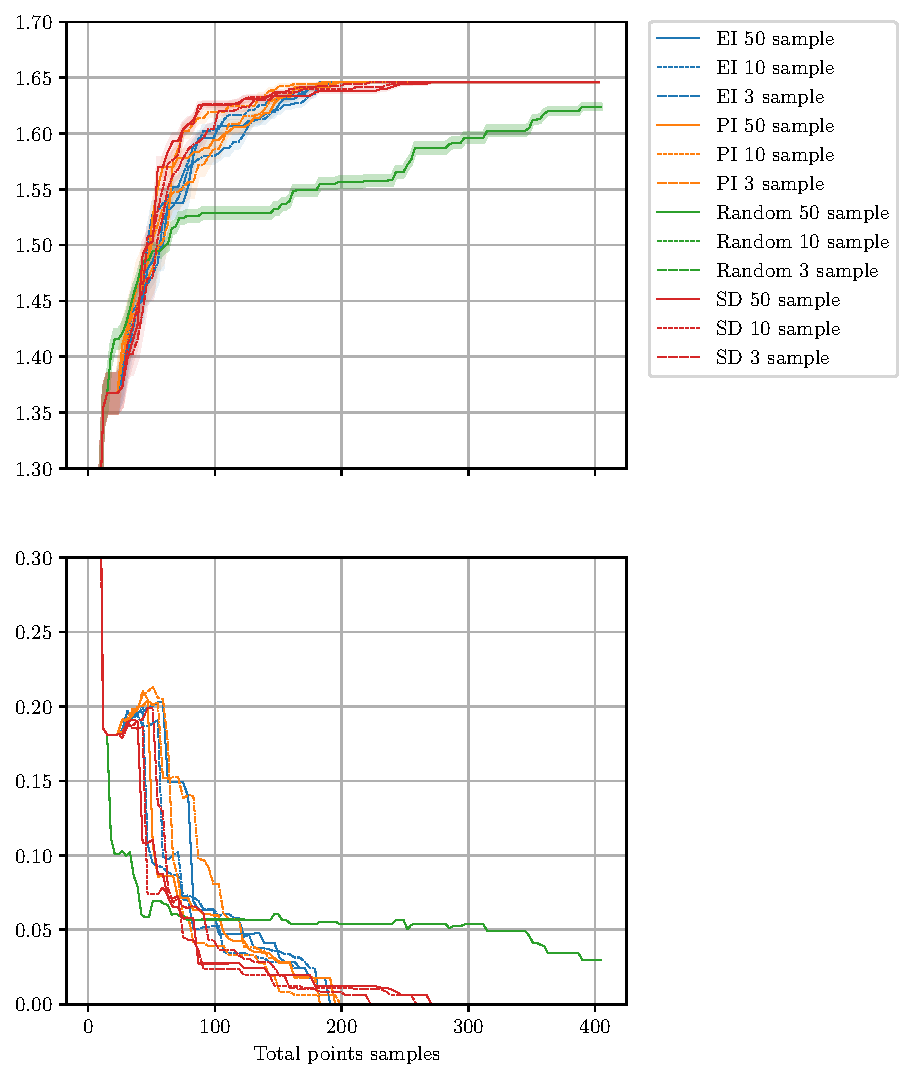
\includegraphics[width=\textwidth]{\dataset/search_algorithm_comparison_incremental_synthetic_3_output_incremental_long}
%		\caption{GPAR 3 training checkpoints model}
%	\end{subfigure}
%	\begin{subfigure}{0.48\textwidth}
%		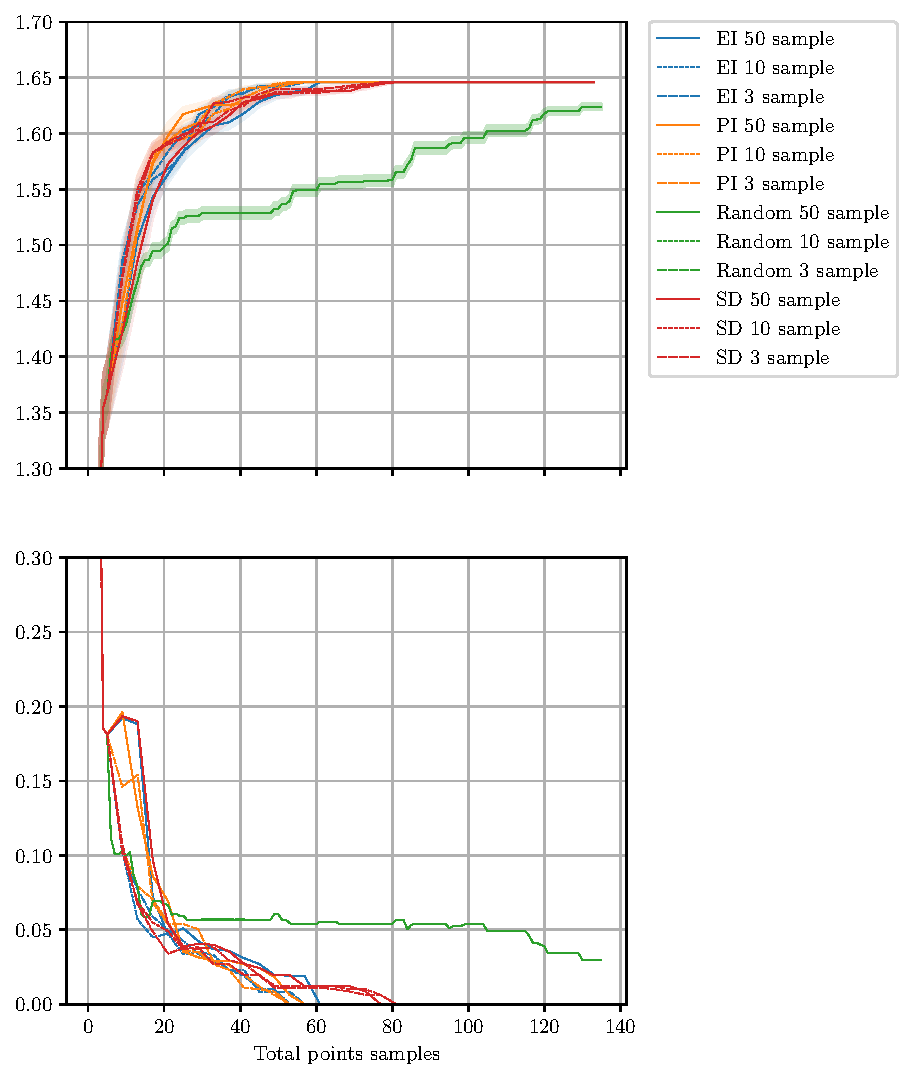
\includegraphics[width=\textwidth]{\dataset/search_algorithm_comparison_incremental_synthetic_3_output_long}
%		\caption{Final performance only model}
%	\end{subfigure}
%	\caption{The search efficiency of tested methods for MLP BNNs on the \dataname\quad dataset. Acquisition functions used are Expected Improvement (EI), Probability of Improvement (PI), Upper Confidence Bound (SD) and random search. 50, 10, and 3 samples were tried for estimating the mean and variance of the GP posterior function.}
%	\label{fig:searches_\dataset}
%\end{figure}

%\begin{figure}[p]
%	\def\dataset{\bostonvar}
%	\def\dataname{\bostonname}
%	\begin{subfigure}{0.48\textwidth}
%		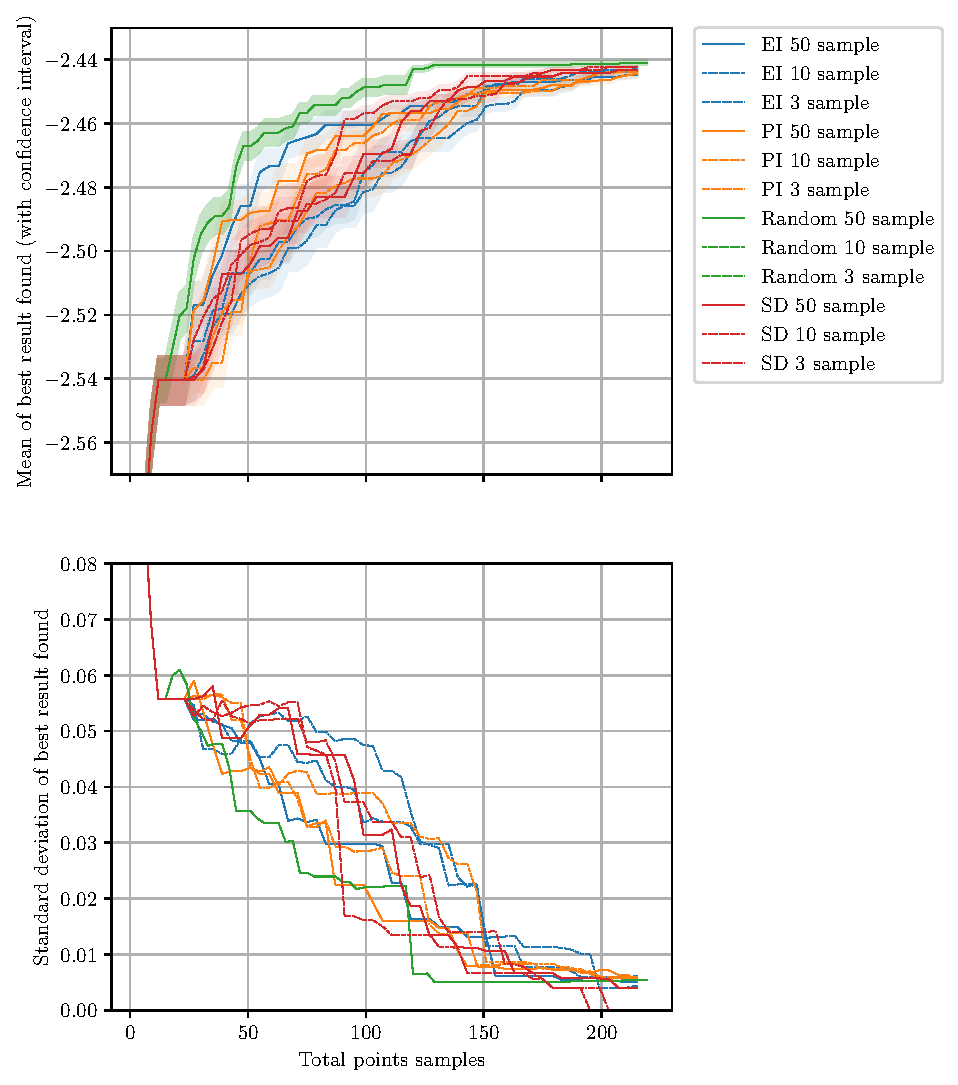
\includegraphics[width=\textwidth]{\dataset/search_algorithm_comparison_output_incremental_long}
%		\caption{\dataname}
%		\label{fig:hidden_width_\dataset}
%	\end{subfigure}
%	\def\dataset{\concretevar}
%	\def\dataname{\concretename}
%	\begin{subfigure}{0.48\textwidth}
%		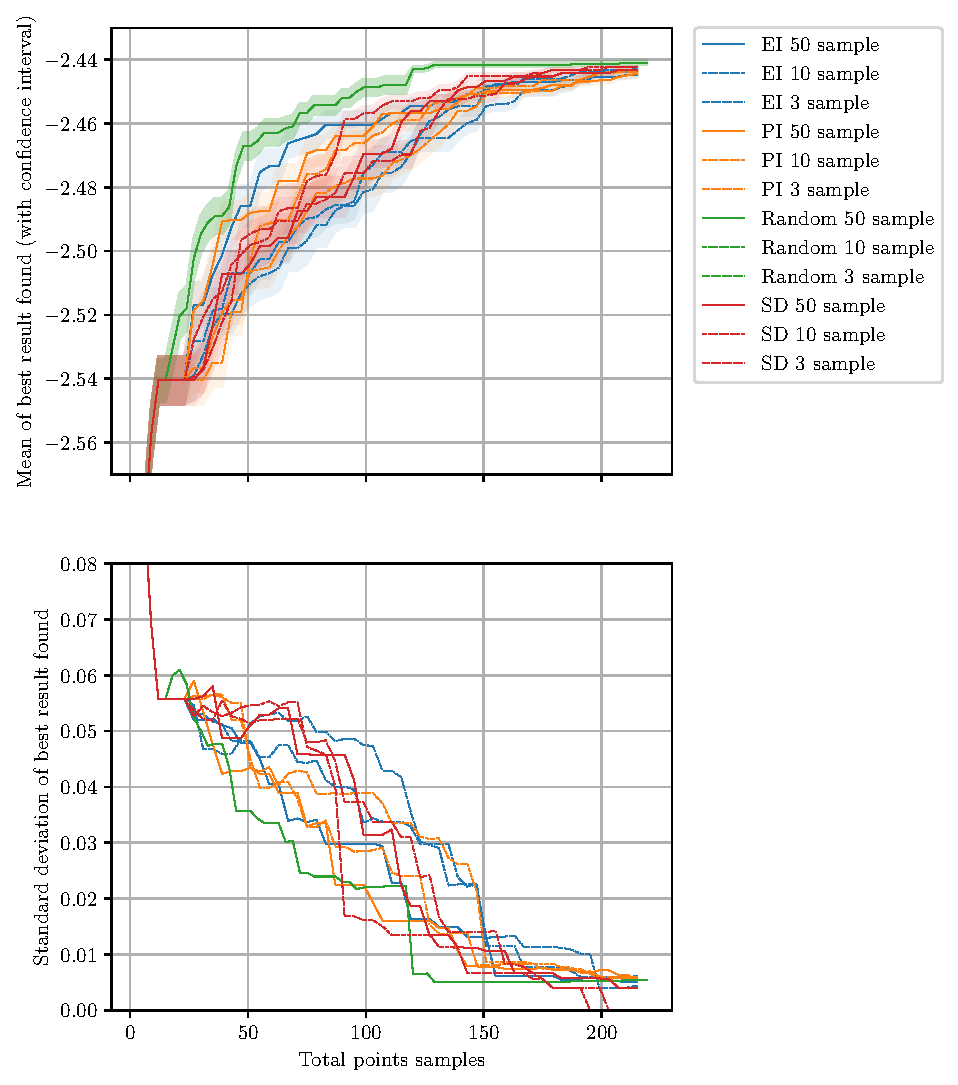
\includegraphics[width=\textwidth]{\dataset/search_algorithm_comparison_output_incremental_long}
%		\caption{\dataname}
%		\label{fig:hidden_width_\dataset}
%	\end{subfigure}
%	
%	\def\dataset{\energyvar}
%	\def\dataname{\energyname}
%	\begin{subfigure}{0.48\textwidth}
%		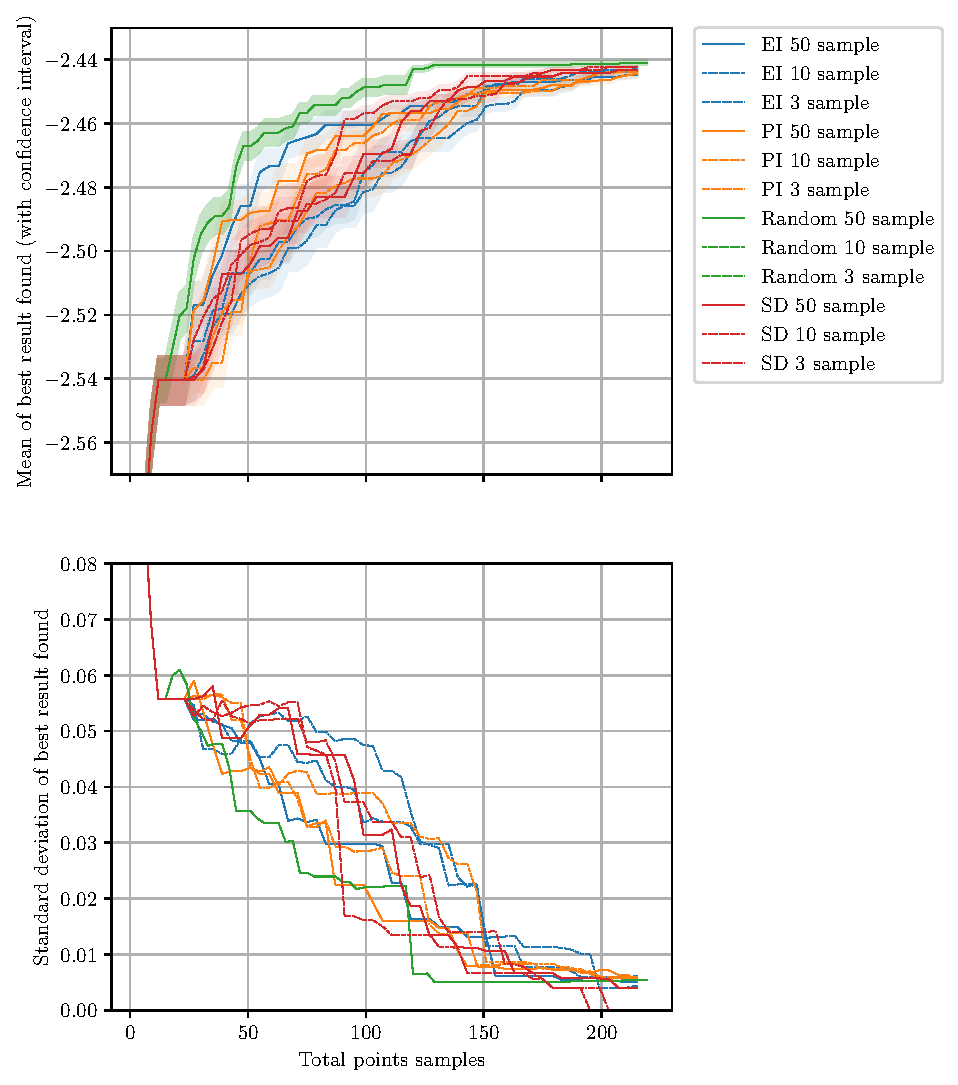
\includegraphics[width=\textwidth]{\dataset/search_algorithm_comparison_output_incremental_long}
%		\caption{\dataname}
%		\label{fig:hidden_width_\dataset}
%	\end{subfigure}
%	\def\dataset{\kinvar}
%	\def\dataname{\kinname}
%	\begin{subfigure}{0.48\textwidth}
%		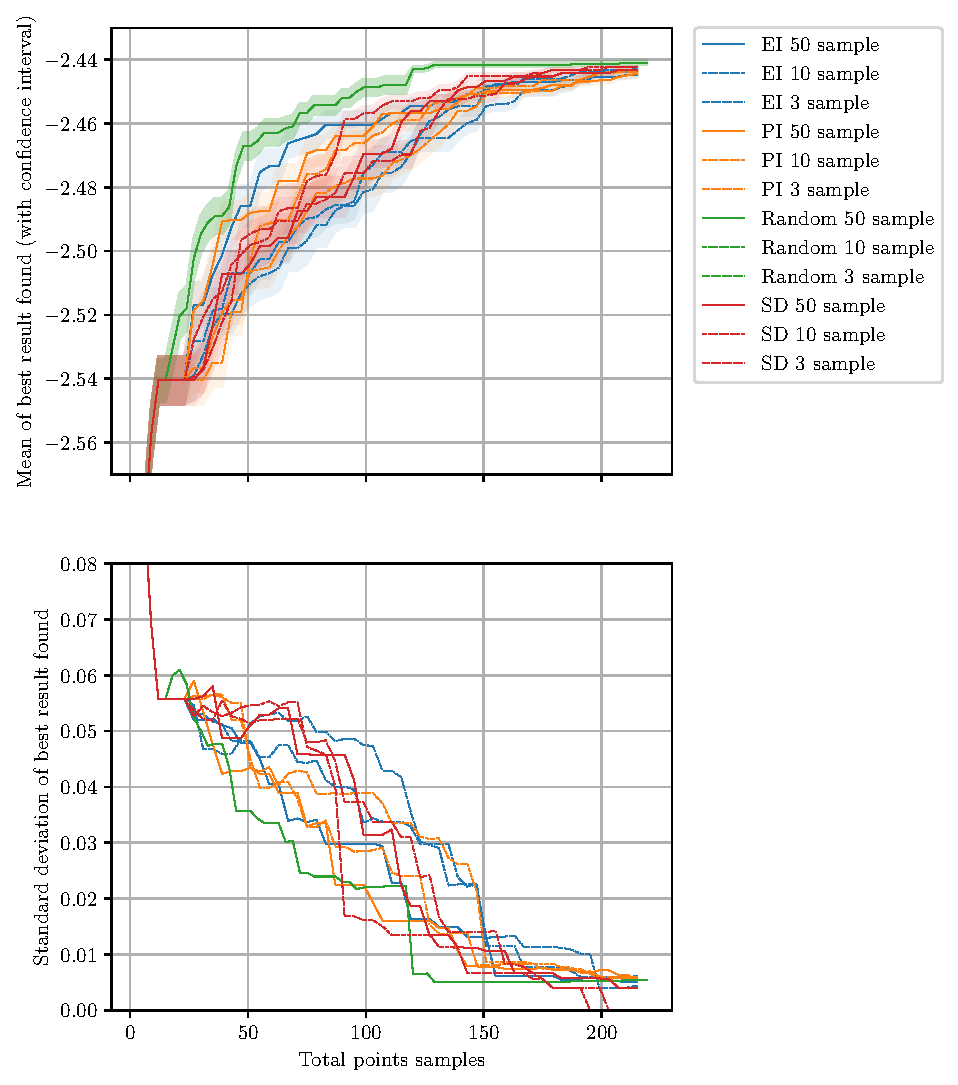
\includegraphics[width=\textwidth]{\dataset/search_algorithm_comparison_output_incremental_long}
%		\caption{\dataname}
%		\label{fig:hidden_width_\dataset}
%	\end{subfigure}
%	\caption{The search efficiency of searching the architecture space of MLP BNNs on various datasets, utilising the GPAR method with 3 checkpoints of training monitored. Acquisition function used are Expected Improvement (EI), Probability of Improvement (PI), Upper Confidence Bound (SD) and random search. 50, 10, and 3 samples were tried for estimating the mean and variance of the GP posterior function.}
%	\label{fig:gpar_1}
%\end{figure}
%
%\begin{figure}[p]
%	\def\dataset{\powervar}
%	\def\dataname{\powername}
%	\begin{subfigure}{0.48\textwidth}
%		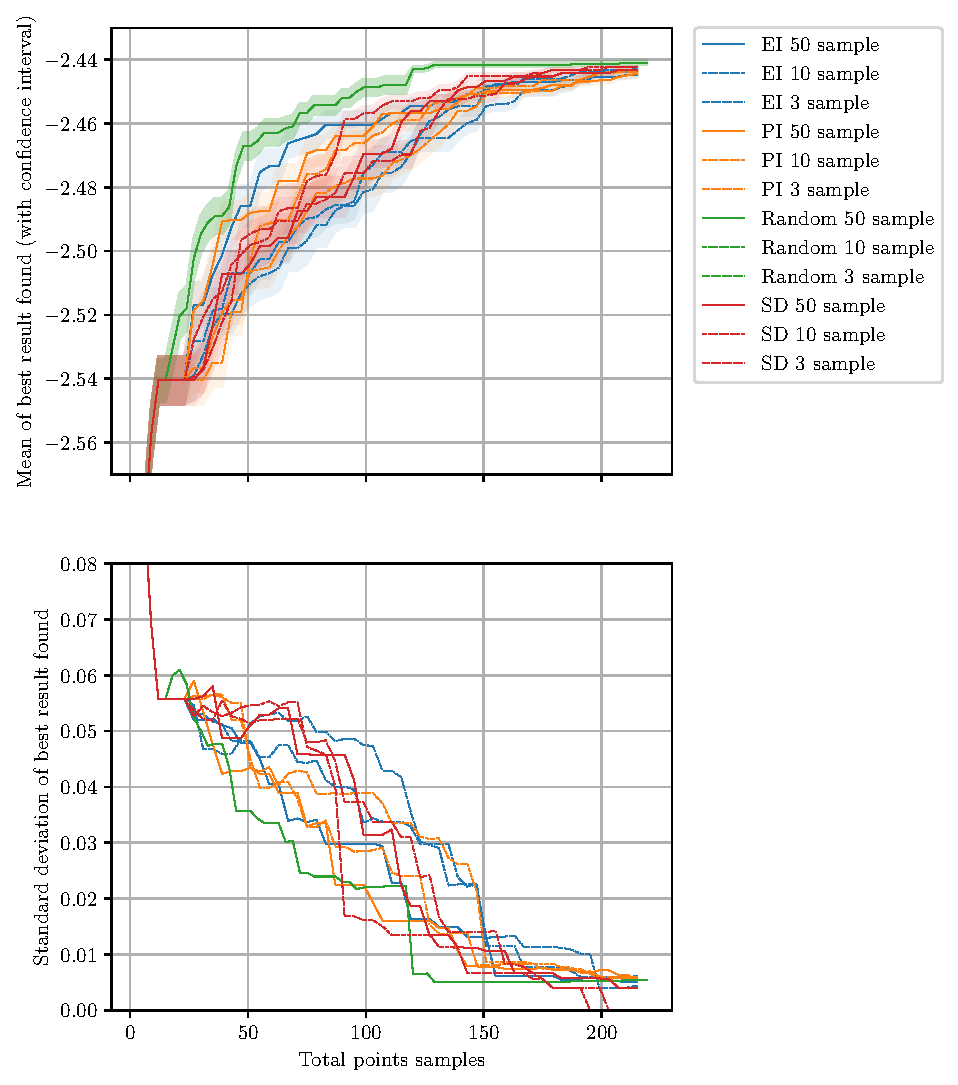
\includegraphics[width=\textwidth]{\dataset/search_algorithm_comparison_output_incremental_long}
%		\caption{\dataname}
%		\label{fig:hidden_width_\dataset}
%	\end{subfigure}
%%	\def\dataset{\proteinvar}
%%	\def\dataname{\proteinname}
%%	\begin{subfigure}{0.48\textwidth}
%%		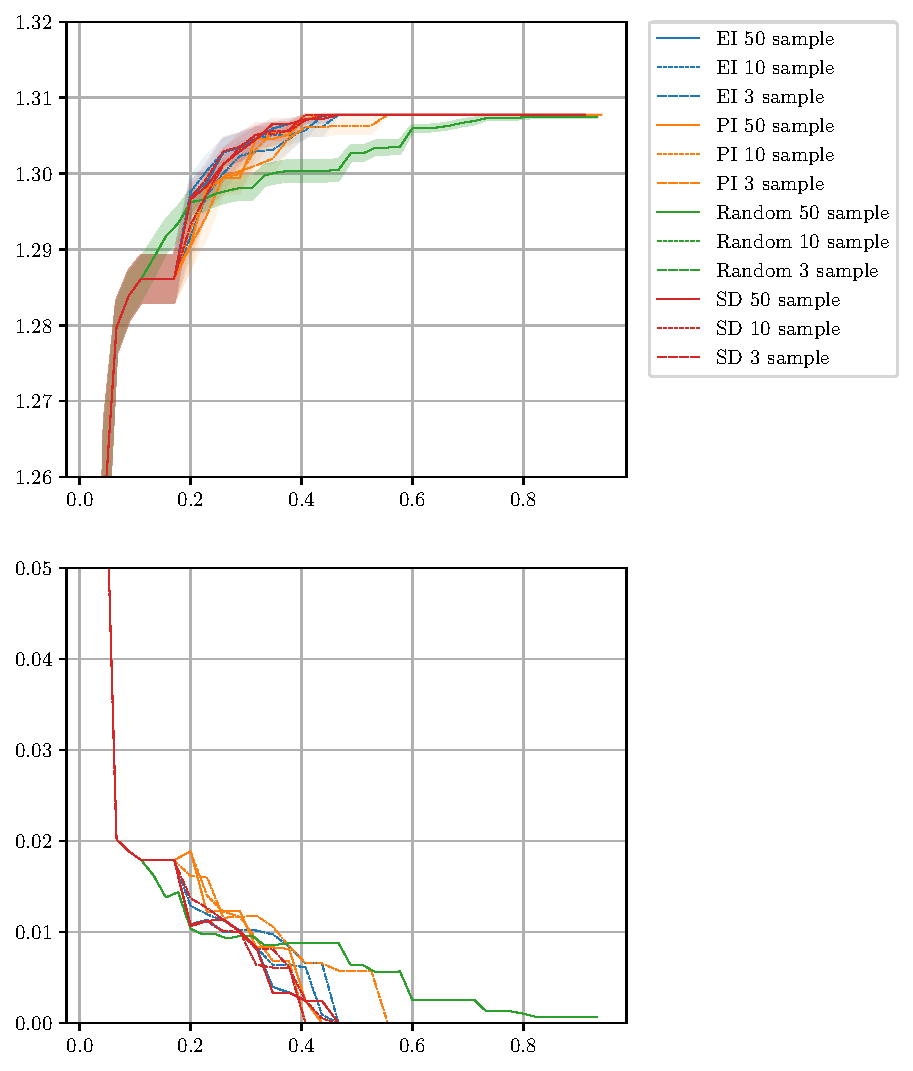
\includegraphics[width=\textwidth]{\dataset/search_algorithm_comparison}
%%		\caption{\dataname}
%%		\label{fig:pruning_\dataset}
%%	\end{subfigure}
%	
%	\def\dataset{\winevar}
%	\def\dataname{\winename}
%	\begin{subfigure}{0.48\textwidth}
%		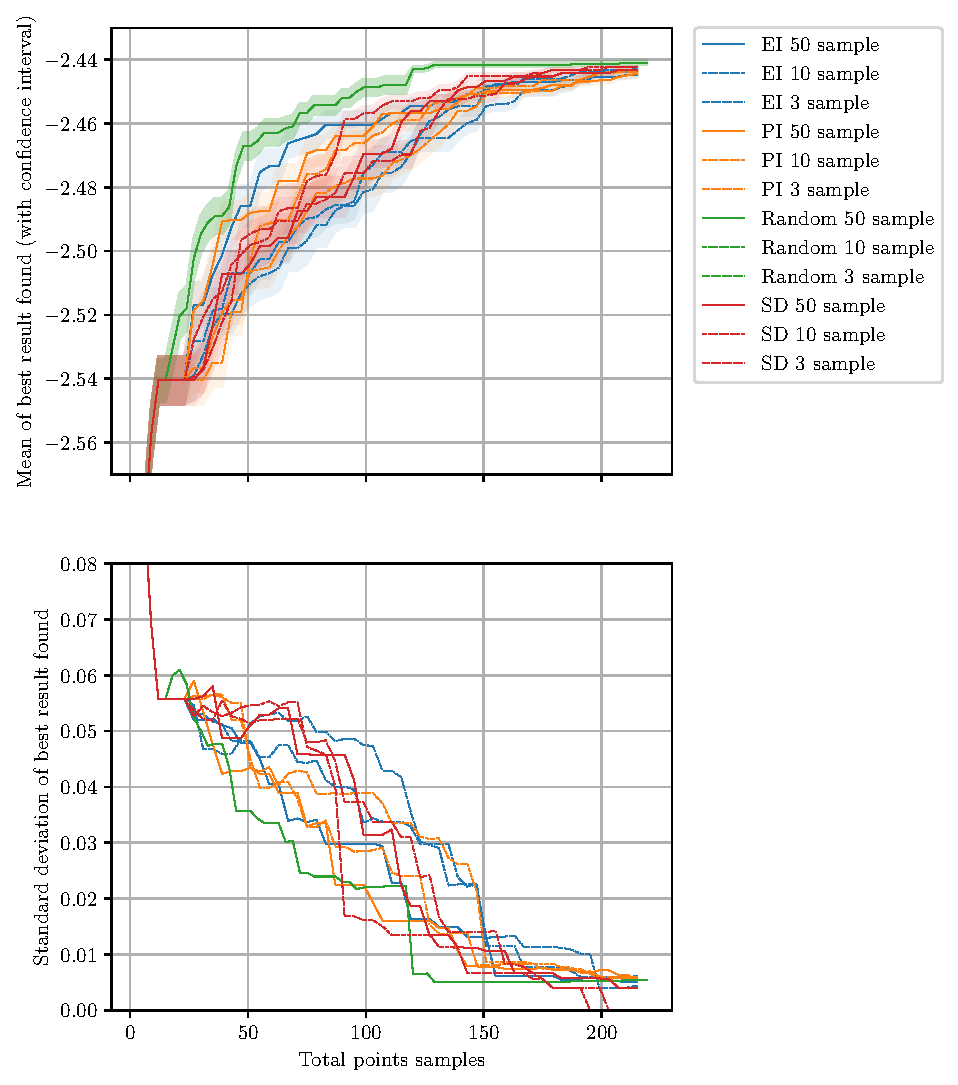
\includegraphics[width=\textwidth]{\dataset/search_algorithm_comparison_output_incremental_long}
%		\caption{\dataname}
%		\label{fig:hidden_width_\dataset}
%	\end{subfigure}
%	\def\dataset{\yachtnvar}
%	\def\dataname{\yachtname}
%	\begin{subfigure}{0.48\textwidth}
%		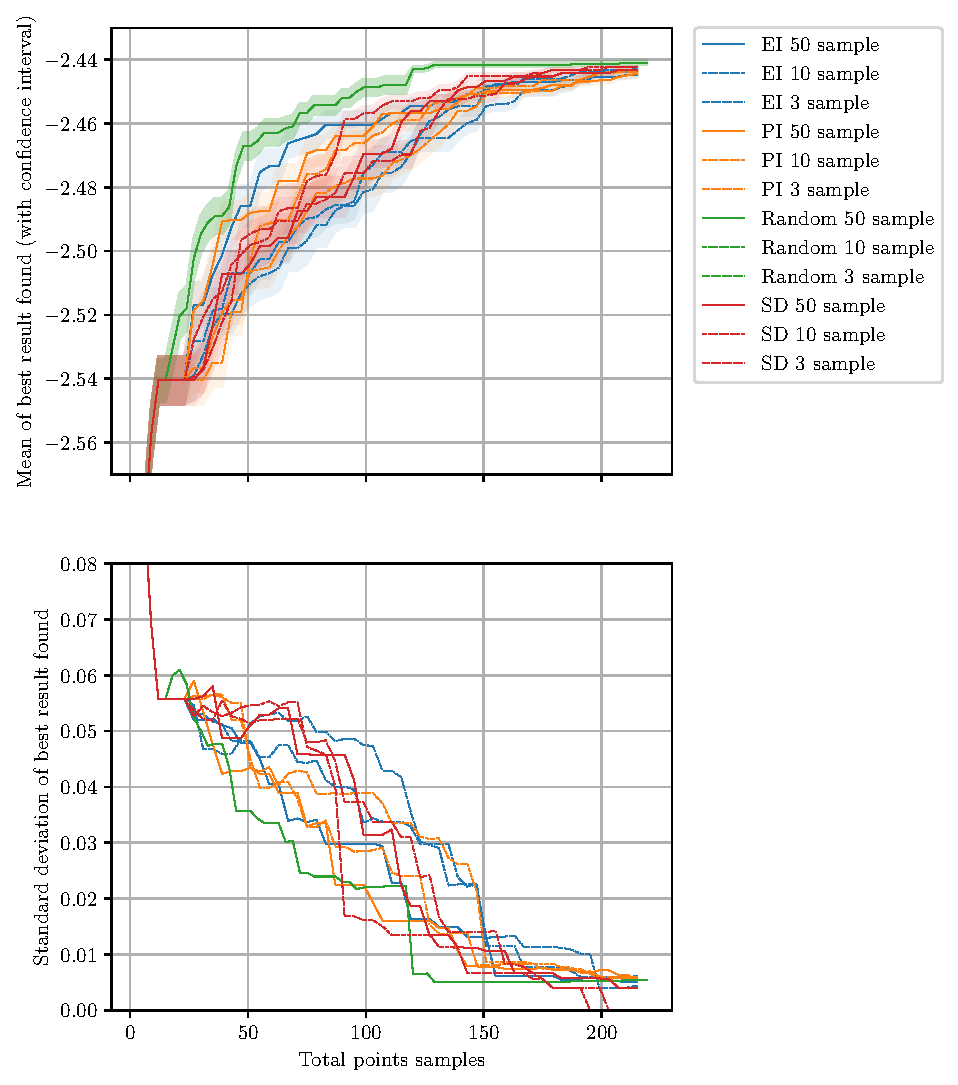
\includegraphics[width=\textwidth]{\dataset/search_algorithm_comparison_output_incremental_long}
%		\caption{\dataname}
%		\label{fig:hidden_width_\dataset}
%	\end{subfigure}
%	
%	\caption{The search efficiency of searching the architecture space of MLP BNNs on various datasets, utilising the GPAR method with 3 checkpoints of training monitored. Acquisition function used are Expected Improvement (EI), Probability of Improvement (PI), Upper Confidence Bound (SD) and random search. 50, 10, and 3 samples were tried for estimating the mean and variance of the GP posterior function.}
%	\label{fig:gpar_2}
%\end{figure}
%
%\begin{figure}[p]
%	\def\dataset{\bostonvar}
%	\def\dataname{\bostonname}
%	\begin{subfigure}{0.48\textwidth}
%		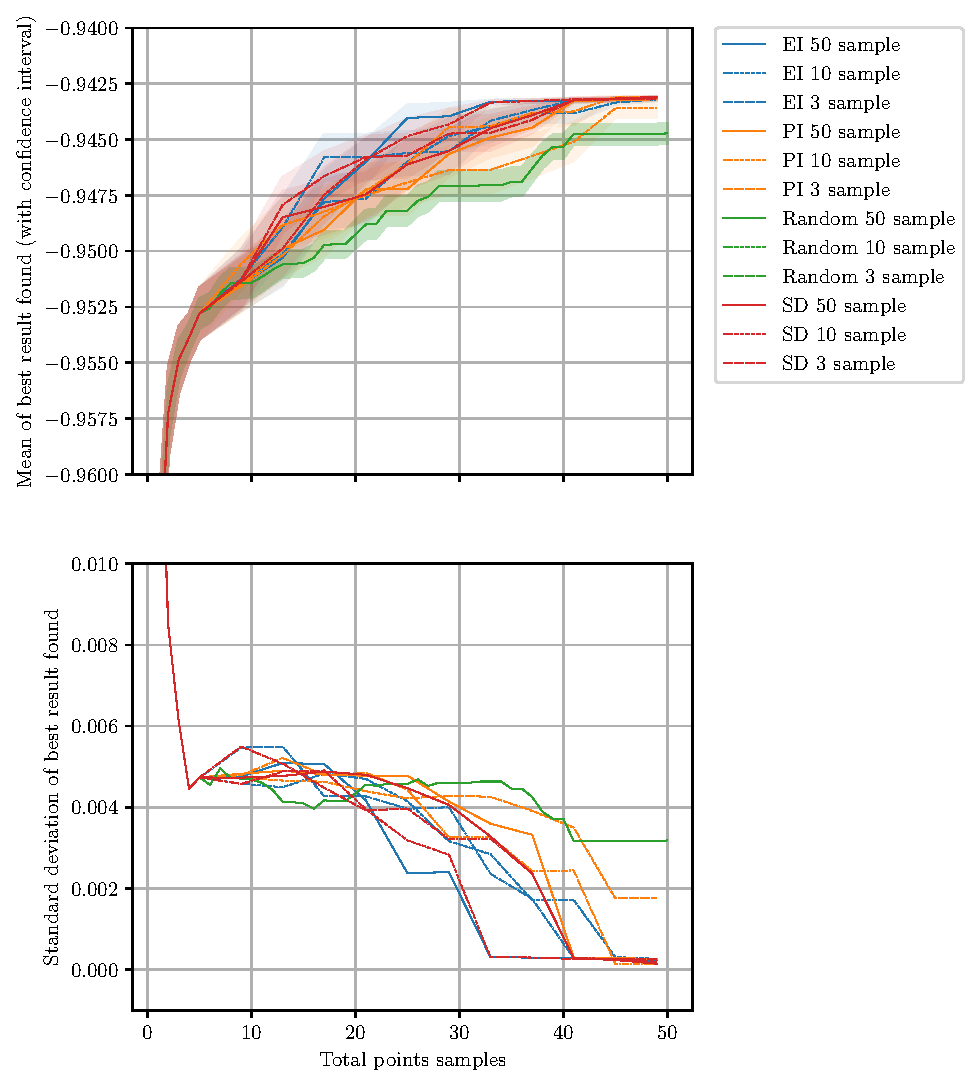
\includegraphics[width=\textwidth]{\dataset/search_algorithm_comparison_output_long}
%		\caption{\dataname}
%		\label{fig:hidden_width_\dataset}
%	\end{subfigure}
%	\def\dataset{\concretevar}
%	\def\dataname{\concretename}
%	\begin{subfigure}{0.48\textwidth}
%		\includegraphics[width=\textwidth]{\dataset/search_algorithm_comparison_output_long}
%		\caption{\dataname}
%		\label{fig:hidden_width_\dataset}
%	\end{subfigure}
%	
%	\def\dataset{\energyvar}
%	\def\dataname{\energyname}
%	\begin{subfigure}{0.48\textwidth}
%		\includegraphics[width=\textwidth]{\dataset/search_algorithm_comparison_output_long}
%		\caption{\dataname}
%		\label{fig:hidden_width_\dataset}
%	\end{subfigure}
%	\def\dataset{\kinvar}
%	\def\dataname{\kinname}
%	\begin{subfigure}{0.48\textwidth}
%		\includegraphics[width=\textwidth]{\dataset/search_algorithm_comparison_output_long}
%		\caption{\dataname}
%		\label{fig:hidden_width_\dataset}
%	\end{subfigure}
%	\caption{The search efficiency of searching the architecture space of MLP BNNs on various datasets, utilising the GPAR method with 3 checkpoints of training monitored. Acquisition function used are Expected Improvement (EI), Probability of Improvement (PI), Upper Confidence Bound (SD) and random search. 50, 10, and 3 samples were tried for estimating the mean and variance of the GP posterior function.}
%	\label{fig:final_1}
%\end{figure}
%
%\begin{figure}[p]
%	\def\dataset{\powervar}
%	\def\dataname{\powername}
%	\begin{subfigure}{0.48\textwidth}
%		\includegraphics[width=\textwidth]{\dataset/search_algorithm_comparison_output_long}
%		\caption{\dataname}
%		\label{fig:hidden_width_\dataset}
%	\end{subfigure}
%	%	\def\dataset{\proteinvar}
%	%	\def\dataname{\proteinname}
%	%	\begin{subfigure}{0.48\textwidth}
%	%		\includegraphics[width=\textwidth]{\dataset/search_algorithm_comparison}
%	%		\caption{\dataname}
%	%		\label{fig:pruning_\dataset}
%	%	\end{subfigure}
%	
%	\def\dataset{\winevar}
%	\def\dataname{\winename}
%	\begin{subfigure}{0.48\textwidth}
%		\includegraphics[width=\textwidth]{\dataset/search_algorithm_comparison_output_long}
%		\caption{\dataname}
%		\label{fig:hidden_width_\dataset}
%	\end{subfigure}
%	\def\dataset{\yachtnvar}
%	\def\dataname{\yachtname}
%	\begin{subfigure}{0.48\textwidth}
%		\includegraphics[width=\textwidth]{\dataset/search_algorithm_comparison_output_long}
%		\caption{\dataname}
%		\label{fig:hidden_width_\dataset}
%	\end{subfigure}
%	
%	\caption{The search efficiency of searching the architecture space of MLP BNNs on various datasets, utilising the GPAR method with 3 checkpoints of training monitored. Acquisition function used are Expected Improvement (EI), Probability of Improvement (PI), Upper Confidence Bound (SD) and random search. 50, 10, and 3 samples were tried for estimating the mean and variance of the GP posterior function.}
%	\label{fig:final_2}
%\end{figure}

\begin{figure}[p]
	\def\dataset{\bostonvar}
	\def\dataname{\bostonname}
	\begin{subfigure}{0.48\textwidth}
		\includegraphics[width=\textwidth]{\dataset/search_algorithm_comparison_output_incremental_long}
		\caption{GPAR 3 training checkpoints model}
	\end{subfigure}
	\begin{subfigure}{0.48\textwidth}
		\includegraphics[width=\textwidth]{\dataset/search_algorithm_comparison_output_long}
		\caption{Final performance only model}
	\end{subfigure}
	\caption{The search efficiency of tested methods for MLP BNNs on the \dataname\quad dataset. Acquisition functions used are Expected Improvement (EI), Probability of Improvement (PI), Upper Confidence Bound (SD) and random search. 50, 10, and 3 samples were tried for estimating the mean and variance of the GP posterior function.}
	\label{fig:searches_\dataset}
\end{figure}

\begin{figure}[p]
	\def\dataset{\concretevar}
	\def\dataname{\concretename}
	\begin{subfigure}{0.48\textwidth}
		\includegraphics[width=\textwidth]{\dataset/search_algorithm_comparison_output_incremental_long}
		\caption{GPAR 3 training checkpoints model}
	\end{subfigure}
	\begin{subfigure}{0.48\textwidth}
		\includegraphics[width=\textwidth]{\dataset/search_algorithm_comparison_output_long}
		\caption{Final performance only model}
	\end{subfigure}
	\caption{The search efficiency of tested methods for MLP BNNs on the \dataname\quad dataset. Acquisition functions used are Expected Improvement (EI), Probability of Improvement (PI), Upper Confidence Bound (SD) and random search. 50, 10, and 3 samples were tried for estimating the mean and variance of the GP posterior function.}
	\label{fig:searches_\dataset}
\end{figure}

\begin{figure}[p]
	\def\dataset{\energyvar}
	\def\dataname{\energyname}
	\begin{subfigure}{0.48\textwidth}
		\includegraphics[width=\textwidth]{\dataset/search_algorithm_comparison_output_incremental_long}
		\caption{GPAR 3 training checkpoints model}
	\end{subfigure}
	\begin{subfigure}{0.48\textwidth}
		\includegraphics[width=\textwidth]{\dataset/search_algorithm_comparison_output_long}
		\caption{Final performance only model}
	\end{subfigure}
	\caption{The search efficiency of tested methods for MLP BNNs on the \dataname\quad dataset. Acquisition functions used are Expected Improvement (EI), Probability of Improvement (PI), Upper Confidence Bound (SD) and random search. 50, 10, and 3 samples were tried for estimating the mean and variance of the GP posterior function.}
	\label{fig:searches_\dataset}
\end{figure}

\begin{figure}[p]
	\def\dataset{\kinvar}
	\def\dataname{\kinname}
	\begin{subfigure}{0.48\textwidth}
		\includegraphics[width=\textwidth]{\dataset/search_algorithm_comparison_output_incremental_long}
		\caption{GPAR 3 training checkpoints model}
	\end{subfigure}
	\begin{subfigure}{0.48\textwidth}
		\includegraphics[width=\textwidth]{\dataset/search_algorithm_comparison_output_long}
		\caption{Final performance only model}
	\end{subfigure}
	\caption{The search efficiency of tested methods for MLP BNNs on the \dataname\quad dataset. Acquisition functions used are Expected Improvement (EI), Probability of Improvement (PI), Upper Confidence Bound (SD) and random search. 50, 10, and 3 samples were tried for estimating the mean and variance of the GP posterior function.}
	\label{fig:searches_\dataset}
\end{figure}

\begin{figure}[p]
	\def\dataset{\powervar}
	\def\dataname{\powername}
	\begin{subfigure}{0.48\textwidth}
		\includegraphics[width=\textwidth]{\dataset/search_algorithm_comparison_output_incremental_long}
		\caption{GPAR 3 training checkpoints model}
	\end{subfigure}
	\begin{subfigure}{0.48\textwidth}
		\includegraphics[width=\textwidth]{\dataset/search_algorithm_comparison_output_long}
		\caption{Final performance only model}
	\end{subfigure}
	\caption{The search efficiency of tested methods for MLP BNNs on the \dataname\quad dataset. Acquisition functions used are Expected Improvement (EI), Probability of Improvement (PI), Upper Confidence Bound (SD) and random search. 50, 10, and 3 samples were tried for estimating the mean and variance of the GP posterior function.}
	\label{fig:searches_\dataset}
\end{figure}

\begin{figure}[p]
	\def\dataset{\proteinvar}
	\def\dataname{\proteinname}
	\begin{subfigure}{0.48\textwidth}
		\includegraphics[width=\textwidth]{\dataset/search_algorithm_comparison_output_incremental_long}
		\caption{GPAR 3 training checkpoints model}
	\end{subfigure}
	\begin{subfigure}{0.48\textwidth}
		\includegraphics[width=\textwidth]{\dataset/search_algorithm_comparison_output_long}
		\caption{Final performance only model}
	\end{subfigure}
	\caption{The search efficiency of tested methods for MLP BNNs on the \dataname\quad dataset. Acquisition functions used are Expected Improvement (EI), Probability of Improvement (PI), Upper Confidence Bound (SD) and random search. 50, 10, and 3 samples were tried for estimating the mean and variance of the GP posterior function.}
	\label{fig:searches_\dataset}
\end{figure}

\begin{figure}[p]
	\def\dataset{\winevar}
	\def\dataname{\winename}
	\begin{subfigure}{0.48\textwidth}
		\includegraphics[width=\textwidth]{\dataset/search_algorithm_comparison_output_incremental_long}
		\caption{GPAR 3 training checkpoints model}
	\end{subfigure}
	\begin{subfigure}{0.48\textwidth}
		\includegraphics[width=\textwidth]{\dataset/search_algorithm_comparison_output_long}
		\caption{Final performance only model}
	\end{subfigure}
	\caption{The search efficiency of tested methods for MLP BNNs on the \dataname\quad dataset. Acquisition functions used are Expected Improvement (EI), Probability of Improvement (PI), Upper Confidence Bound (SD) and random search. 50, 10, and 3 samples were tried for estimating the mean and variance of the GP posterior function.}
	\label{fig:searches_\dataset}
\end{figure}

\begin{figure}[p]
	\def\dataset{\yachtnvar}
	\def\dataname{\yachtname}
	\begin{subfigure}{0.48\textwidth}
		\includegraphics[width=\textwidth]{\dataset/search_algorithm_comparison_output_incremental_long}
		\caption{GPAR 3 training checkpoints model}
	\end{subfigure}
	\begin{subfigure}{0.48\textwidth}
		\includegraphics[width=\textwidth]{\dataset/search_algorithm_comparison_output_long}
		\caption{Final performance only model}
	\end{subfigure}
	\caption{The search efficiency of tested methods for MLP BNNs on the \dataname\quad dataset. Acquisition functions used are Expected Improvement (EI), Probability of Improvement (PI), Upper Confidence Bound (SD) and random search. 50, 10, and 3 samples were tried for estimating the mean and variance of the GP posterior function.}
	\label{fig:searches_\dataset}
\end{figure}

\begingroup
\let\clearpage\relax
%!TEX root = ../thesis.tex
%*******************************************************************************
%*********************************** Sixth Chapter *****************************
%*******************************************************************************

\chapter{Conclusion}
\label{ch:future_study}

\ifpdf
    \graphicspath{{Chapter6/Figs/Raster/}{Chapter6/Figs/PDF/}{Chapter6/Figs/}}
\else
    \graphicspath{{Chapter6/Figs/Vector/}{Chapter6/Figs/}}
\fi

Presented here are two main groups of contributions. 

First, a detailed study of the effects of various hyper-parameters on the performance of MLP structure BNNs, and identification of systematic trends. We find that layer width and depth are both important factors. Networks that are too large can be detrimental to performance. The effect of the amount of data in the training set has on model optimisation is also investigated. It is shown that the balance between model size and data size is important in controlling the under-fitting or over-fitting of models. Finally the effects of pruning in VI BNNs investigated, and the manner in which the optimiser makes the trade off between reconstruction loss and prior fit terms. We find that in larger networks, many of the weights are pruned completely out the model, reducing the model to a minimum descriptive length, or in some cases further.

Second, is a new method for searching for optimal MLP structure networks in Bayesian Neural Networks, a task currently untackled. This method robustly outperforms the random search on the majority of tasks, excepting cases where the noise from randomness in training BNNs is too great. In most tasks it is as good as, or marginally better than simply performing Bayesian optimisation over the final performance of the BNNs.

\section{Future study}

This thesis represents a first step into architecture search for BNNs. Two directions present themselves as interesting avenues for future work. 

First, a continuation of this specific search method for architecture search, or for hyper-parameter optimisation in general. The ability to incorporate information from snapshots of time during training to allow for early stopping is a reasonably uncommon property in search mechanisms, and this method presented here is entirely novel.

Several immediate improvements could be investigated. The current acquisition functions used are inherently greedy algorithms. Trading off for some additional exploration may help the search rapidly identify good regions to explore. \citet{Brochu2010a} investigates methods for altering the exploration-exploitation balance in the acquisition functions used in this project. \citet{Ginsbourger2008} introduces methodology to do parallel processing EI Bayesian optimisation. Instead of the stochastic noise introduced in this project to diversify the selected search points, this work introduces multi-step optimal acquisition functions that may provide significant gains in performance of this model. \citet{Hennig2012} proposes a new acquisition function that attempts to minimise the entropy of the predictive models posterior. The objective of this is to optimally find the \textit{location} of the maximum, not necessarily explore it. Application of this to the search space may speed up the process of finding the location of optimal architectures.

The other line of investigation is to apply some of the more modern architecture search techniques to BNNs. Recent efforts have	 shown promising initial results in scaling BNNs to the size of some larger CNN models \cite{Shridhar2018,richtalkBNNscale}, and so automated search becomes even more important at this scale. It is not immediately clear how to apply network morphisms or one-shot modelling to BNNs, key components in efficient large scale search, but the results of this would be intriguing to investigate.
\endgroup
%\include{Chapter7/chapter7}

\let\clearpage\relax
\begin{appendices}	
	\section*{Appendix A: Risk Assessment Retrospective}
	
	The main and only risk assessed surrounding this project was the extensive computer work that would be required. This proved to be true. The measures detailed in the risk assessment - taking regular breaks from using the computer, and ensuring good posture - were followed and injuries were sustained in the course of this project. 
\end{appendices}

\pagebreak

% ********************************** Back Matter *******************************
% Backmatter should be commented out, if you are using appendices after References
%\backmatter

% ********************************** Bibliography ******************************
\begin{spacing}{0.9}

% To use the conventional natbib style referencing
% Bibliography style previews: http://nodonn.tipido.net/bibstyle.php
% Reference styles: http://sites.stat.psu.edu/~surajit/present/bib.htm

\bibliographystyle{apalike}
%\bibliographystyle{unsrt} % Use for unsorted references  
%\bibliographystyle{plainnat} % use this to have URLs listed in References
\cleardoublepage

\small
\pagenumbering{gobble}
\bibliography{References/mendeley} % Path to your References.bib file

% If you would like to use BibLaTeX for your references, pass `custombib' as
% an option in the document class. The location of 'reference.bib' should be
% specified in the preamble.tex file in the custombib section.
% Comment out the lines related to natbib above and uncomment the following line.

%\printbibliography[heading=bibintoc, title={References}]


\end{spacing}


\end{document}
